\documentclass[compress]{beamer}
\usepackage{ifthen,verbatim}

\newcommand{\isnote}{}
\xdefinecolor{lightyellow}{rgb}{1.,1.,0.25}
\xdefinecolor{darkblue}{rgb}{0.1,0.1,0.7}
\xdefinecolor{darkred}{rgb}{0.9,0.,0.}
\xdefinecolor{lightblue}{rgb}{0.2,0.6,0.6}

%% Uncomment this to get annotations
%% \def\notes{\addtocounter{page}{-1}
%%            \renewcommand{\isnote}{*}
%% 	   \beamertemplateshadingbackground{lightyellow}{white}
%%            \begin{frame}
%%            \frametitle{Notes for the previous page (page \insertpagenumber)}
%%            \itemize}
%% \def\endnotes{\enditemize
%% 	      \end{frame}
%%               \beamertemplateshadingbackground{white}{white}
%%               \renewcommand{\isnote}{}}

%% Uncomment this to not get annotations
\def\notes{\comment}
\def\endnotes{\endcomment}

\setbeamertemplate{navigation symbols}{}
\setbeamertemplate{headline}{\mbox{ } \hfill
\begin{minipage}{5.5 cm}
\vspace{-0.75 cm} \small
\end{minipage} \hfill
\begin{minipage}{4.5 cm}
\vspace{-0.75 cm} \small
\begin{flushright}
\ifthenelse{\equal{\insertpagenumber}{1}}{}{Jim Pivarski \hspace{0.2 cm} \insertpagenumber\isnote/\pageref{numpages}}
\end{flushright}
\end{minipage}\mbox{\hspace{0.2 cm}}\includegraphics[height=1 cm]{../cmslogo} \hspace{0.1 cm} \includegraphics[height=1 cm]{../tamulogo} \hspace{0.01 cm} \vspace{-1.05 cm}}

\begin{document}
\begin{frame}
\vfill
\begin{center}
\textcolor{darkblue}{\Large Alignment with Tracks}

\vfill
\begin{columns}
\column{0.3\linewidth}
\begin{center}
\large
\textcolor{darkblue}{Jim Pivarski}

\vspace{0.2 cm}
Alexei Safonov
\end{center}

\column{0.3\linewidth}
\begin{center}
\large
K\'aroly Banicz
\end{center}
\end{columns}

\begin{columns}
\column{0.3\linewidth}
\begin{center}
\scriptsize
{\it Texas A\&M University}
\end{center}
\column{0.3\linewidth}
\begin{center}
\scriptsize
{\it US-CMS}
\end{center}
\end{columns}

\vfill
15 March, 2009

\end{center}
\end{frame}

%% \begin{notes}
%% \item This is the annotated version of my talk.
%% \item If you want the version that I am presenting, download the one
%% labeled ``slides'' on Indico (or just ignore these yellow pages).
%% \item The annotated version is provided for extra detail and a written
%% record of comments that I intend to make orally.
%% \item Yellow notes refer to the content on the {\it previous} page.
%% \item All other slides are identical for the two versions.
%% \end{notes}

\small

\begin{frame}
\frametitle{Since last time\ldots}

\begin{itemize}
\item CSC Overlaps alignment with beam-halo approved for public
\item Cleanly separated $\vec{B}(\vec{x})$ and $dE/dx$ errors from misalignments
\item More complete understanding of residuals (non-Gaussian tails)
\item Began diagnostics of track-source bias in real data
\item Aligned about half of the DT chambers relative to tracker in CRAFT
\end{itemize}

\vfill
\hspace{-0.83 cm} \textcolor{darkblue}{\Large In progress {\large (concurrently)}\ldots}

\begin{itemize}
\item Aligning CSCs relative to barrel using the same CRAFT data
\item Well-organized software framework for push-button CRAFT-2009
\item 50~pb$^{-1}$ Monte Carlo study with updated procedure and systematics
\item CMS Note on HIP procedure and results \mbox{(barrel$+$endcap, cosmics$+$MC)\hspace{-1 cm}}
\end{itemize}

\vfill
\hspace{-0.83 cm} \textcolor{darkblue}{\large At the end of this talk, I'll give a timeline}
\end{frame}

\begin{frame}
\frametitle{Outline for this talk}
\begin{enumerate}\setlength{\itemsep}{0.6 cm}
\item \textcolor{darkblue}{Developments from CRAFT experience}
\begin{itemize}\setlength{\itemsep}{0.2 cm}
\item optimizing procedure to distribution of cosmic rays
\item alignment in the presence of $\vec{B}(\vec{x})$ and $dE/dx$ errors
\item residuals from single-scattering
\item studies of track-source bias
\end{itemize}
\item \textcolor{darkblue}{Global alignment of DT chambers}
\begin{itemize}\setlength{\itemsep}{0.2 cm}
\item cross-checks: not just a residuals minimization
\end{itemize}
\item \textcolor{darkblue}{Preliminary CSC alignment plots from Monte Carlo (statistical only)}
\item \textcolor{darkblue}{Steps toward muon geometry for first collisions and 200~pb$^{-1}$}
\end{enumerate}
%% \hspace{-0.83 cm} \textcolor{darkblue}{\Large Outline2}
\end{frame}

%% \section*{First section}
%% \begin{frame}
%% \begin{center}
%% \Huge \textcolor{blue}{First section}
%% \end{center}
%% \end{frame}

\begin{frame}
\frametitle{Cosmic ray track distribution}
\begin{itemize}
\item We knew from MC that few cosmics would link endcap to tracker
\begin{itemize}
\item standard (collisions) alignment procedure fits tracks with silicon tracker
  and propagates them to each muon chamber
\item only about half of the DTs and ``few if any'' individual CSCs can be
  aligned this way in a several-week cosmic ray run
\end{itemize}

\item Large structures (wheels and disks) can be aligned with \mbox{small statistics\hspace{-1 cm}}
\begin{itemize}
\item but $\phi$ asymmetry hilights some chambers at expense of others
\item whole wheel would rotate to align one or two chambers!
\end{itemize}
\end{itemize}

\begin{columns}
\column{0.45\linewidth}
\textcolor{darkblue}{\large Global alignment plan:}

\begin{enumerate}
\item<alert@1> \textcolor{red}{Align DT chambers individually to tracker}
\item \textcolor{blue}{Complete and cross-check barrel with \mbox{standAlone cosmics\hspace{-1 cm}}}
\item \textcolor{blue}{Align CSC chambers individually to barrel}
\end{enumerate}

\column{0.6\linewidth}
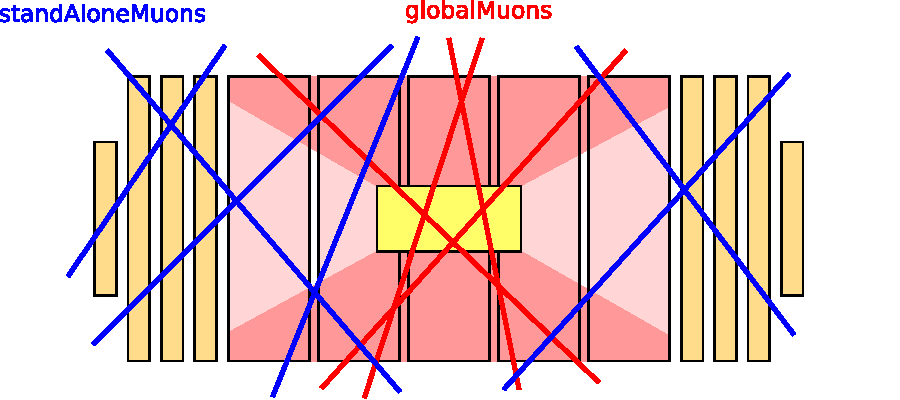
\includegraphics[width=\linewidth]{accessible_to_globalMuons.pdf}
\end{columns}
\end{frame}

\begin{frame}
\frametitle{$\vec{B}(\vec{x})$, $dE/dx$ and misalignment}

\begin{columns}
\column{0.7\linewidth}
\vspace{-0.5 cm}
\begin{itemize}
\item Residuals from misalignment are independent of the tracks used to measure it
\item Residuals from $\vec{B}(\vec{x})$ and $dE/dx$ errors \mbox{flip sign\hspace{-0.5 cm}} with the charge
  of the muon and \mbox{depend on $p_T$\hspace{-1 cm}}
\end{itemize}

\column{0.3\linewidth}
\vspace{0.5 cm}
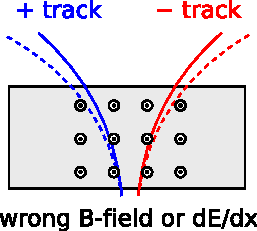
\includegraphics[width=\linewidth]{antisymmetric_bfield.pdf}
\end{columns}

\vspace{-0.2 cm}
\textcolor{darkblue}{\large Two-bin approach:}
\begin{description}
\item[Fact:] momentum spectra for $+$ and $-$ charges are proportional
\item[Fact:] $\vec{B}(\vec{x})$ and $dE/dx$ effects are both antisymmetric with $q$
\end{description}

\begin{columns}
\column{0.5\linewidth}
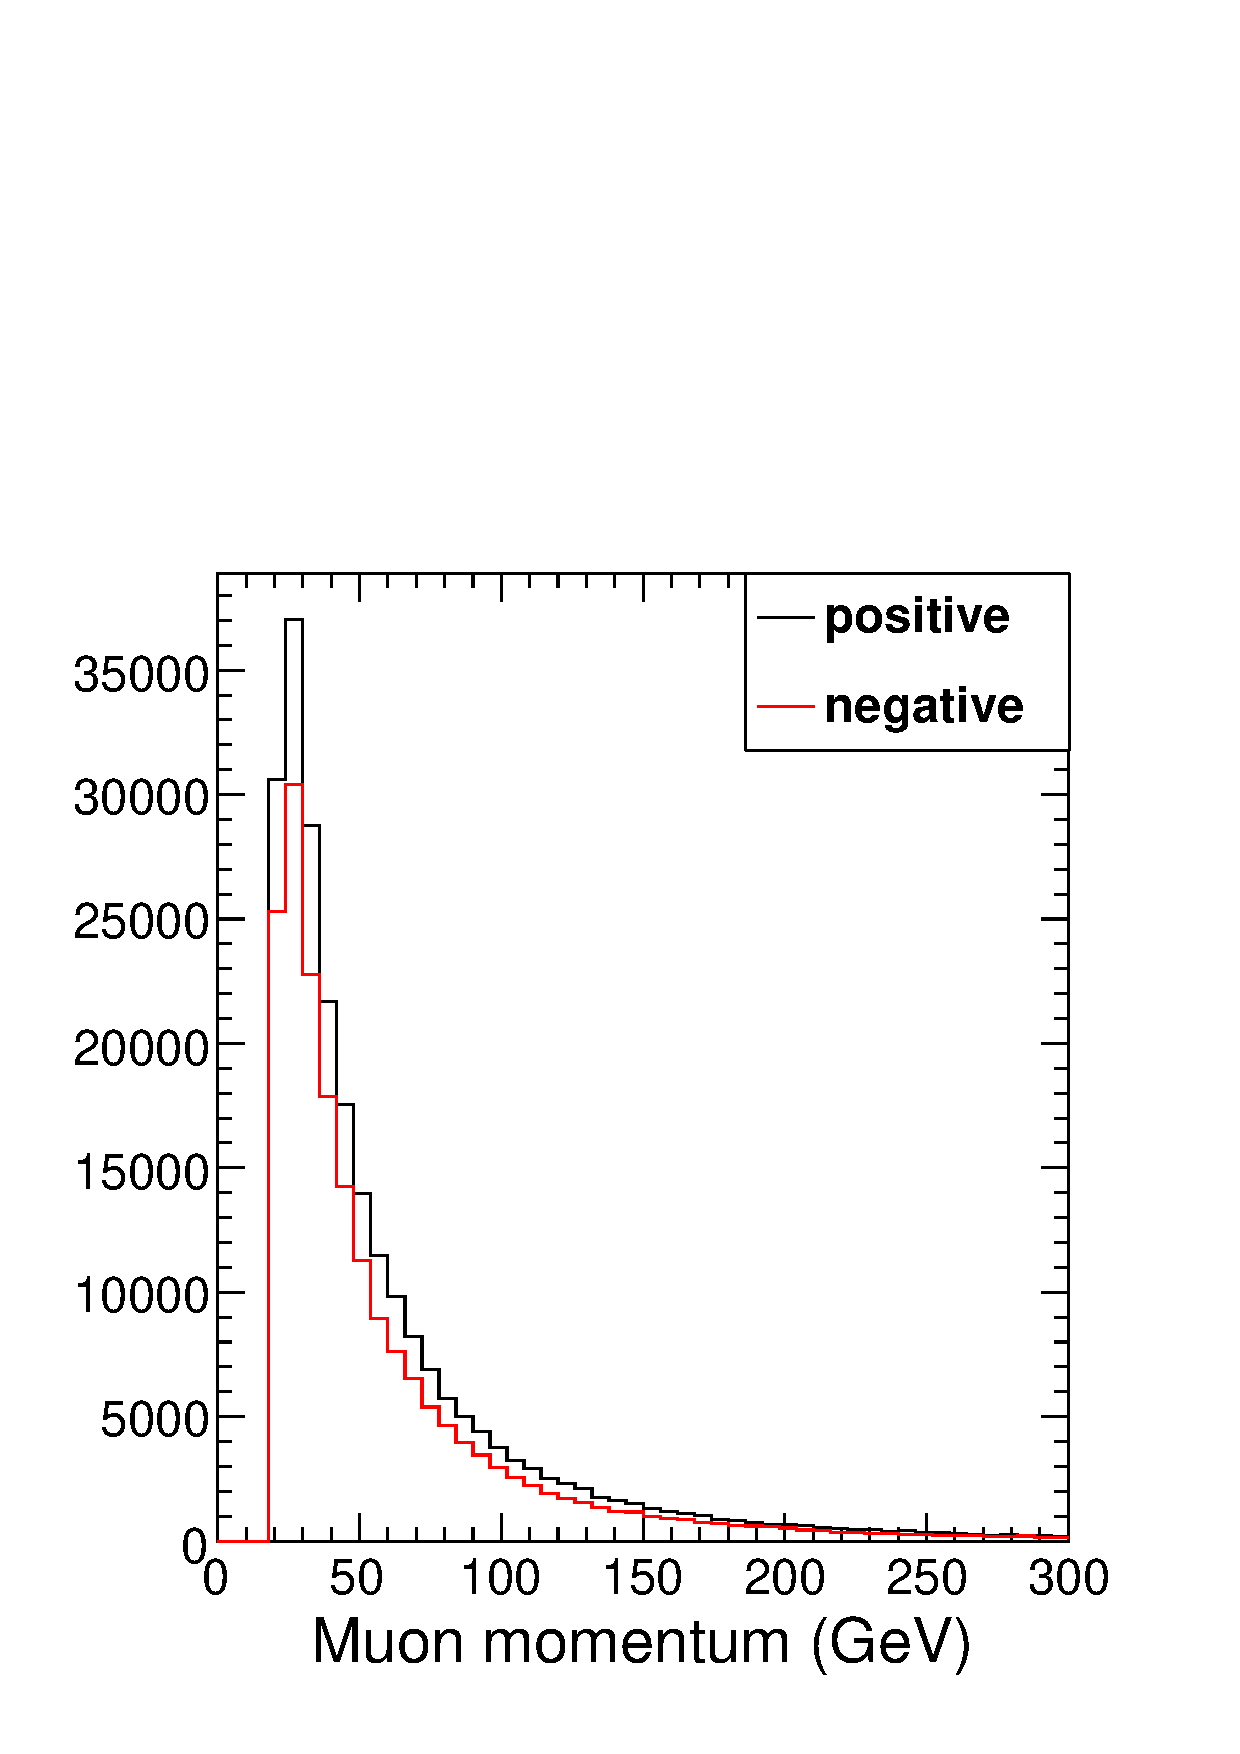
\includegraphics[width=0.5\linewidth]{demo_momentum.pdf}
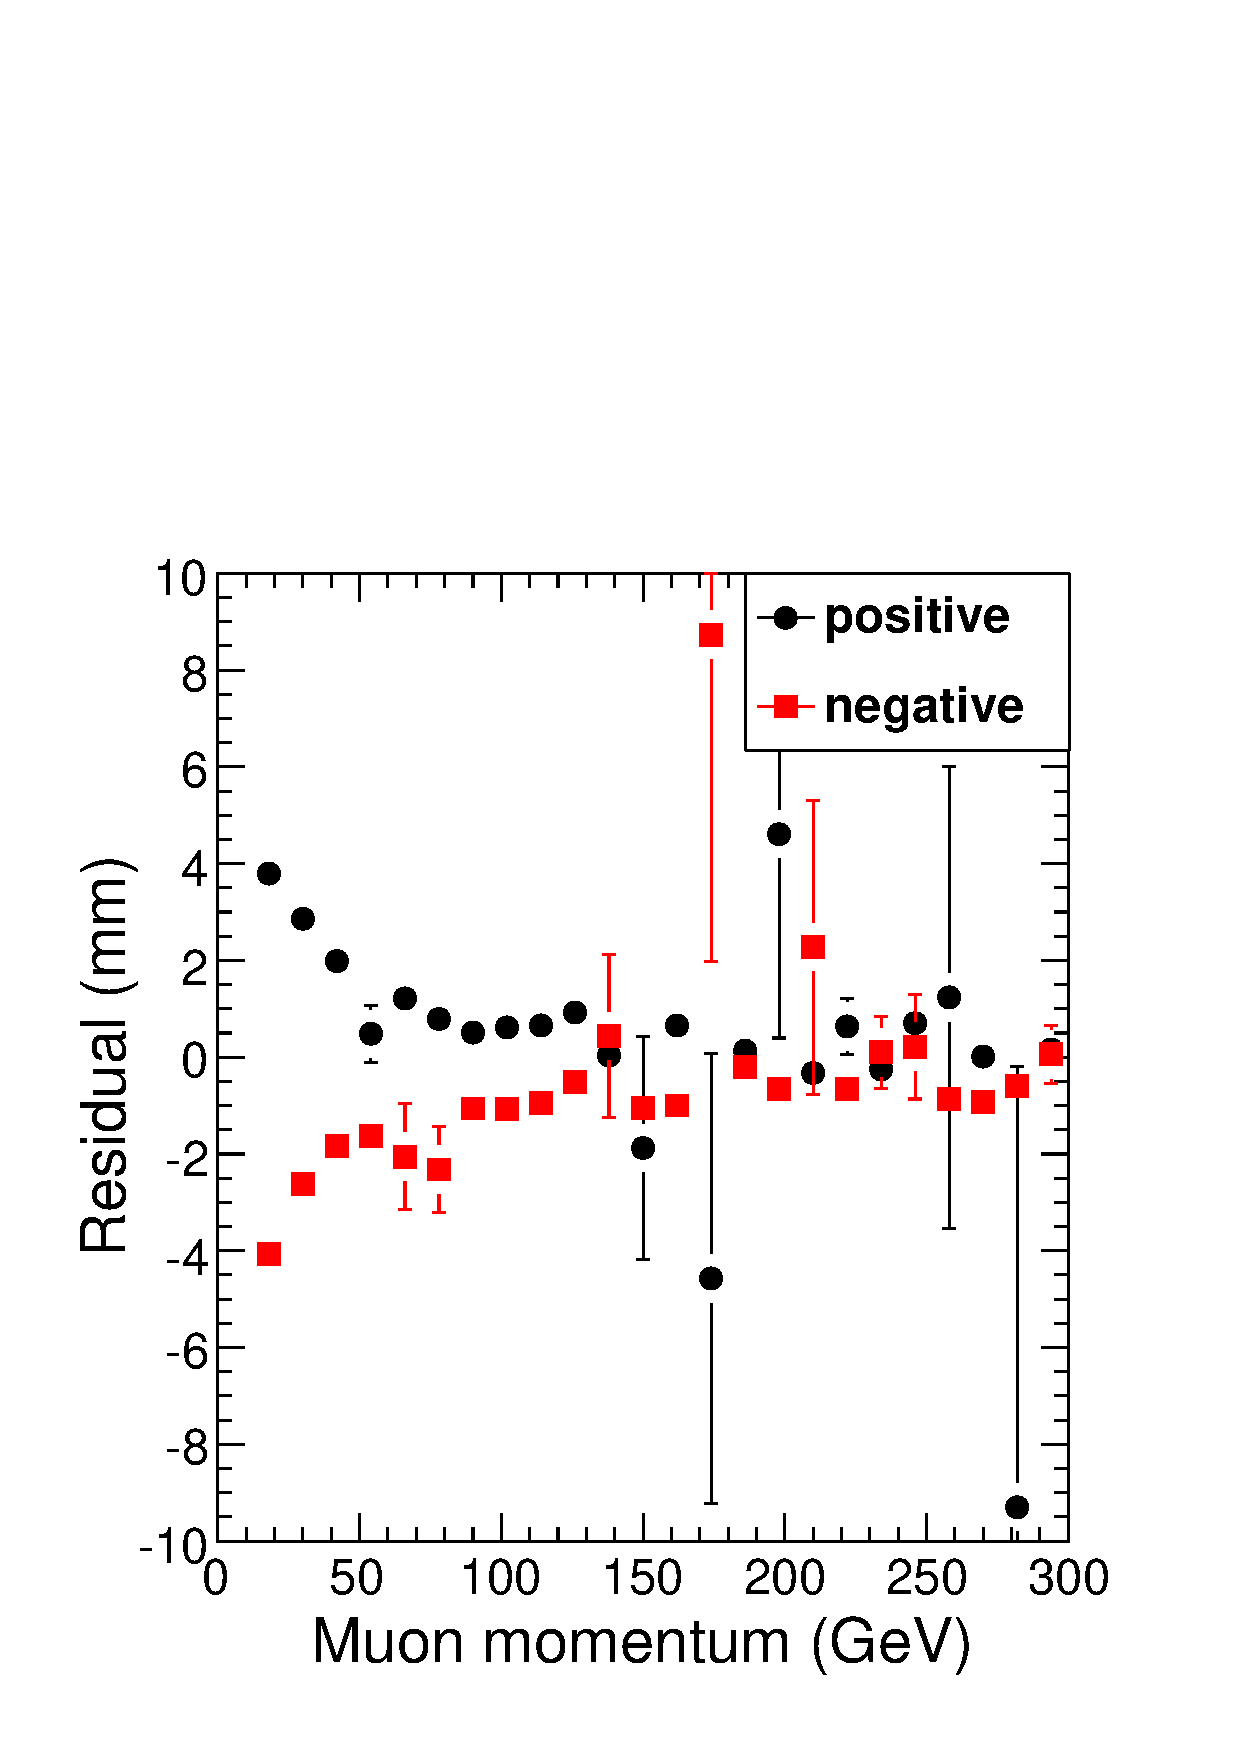
\includegraphics[width=0.5\linewidth]{demo_residual.pdf}

\column{0.6\linewidth}
\begin{itemize}
\item Find peak of residuals in two charge bins: $R_+$ and $R_-$
\item Average $(R_+ + R_-)/2$ is sensitive to misalignment only
\item Difference is sensitive to $\vec{B}$ error and $dE/dx$ errors
  only
\end{itemize}
\vspace{0.3 cm}
\end{columns}
\end{frame}

\begin{frame}
\frametitle{Demonstration in MB4}

\begin{itemize}
\item Station 4 has the largest $\vec{B}$-field errors: plot residuals across barrel
\item The \textcolor{darkred}{misalignment} breaks cleanly at the \mbox{chamber boundaries\hspace{-1 cm}}
\item The \textcolor{lightblue}{$\vec{B}$-field error} is independent of chamber
\end{itemize}

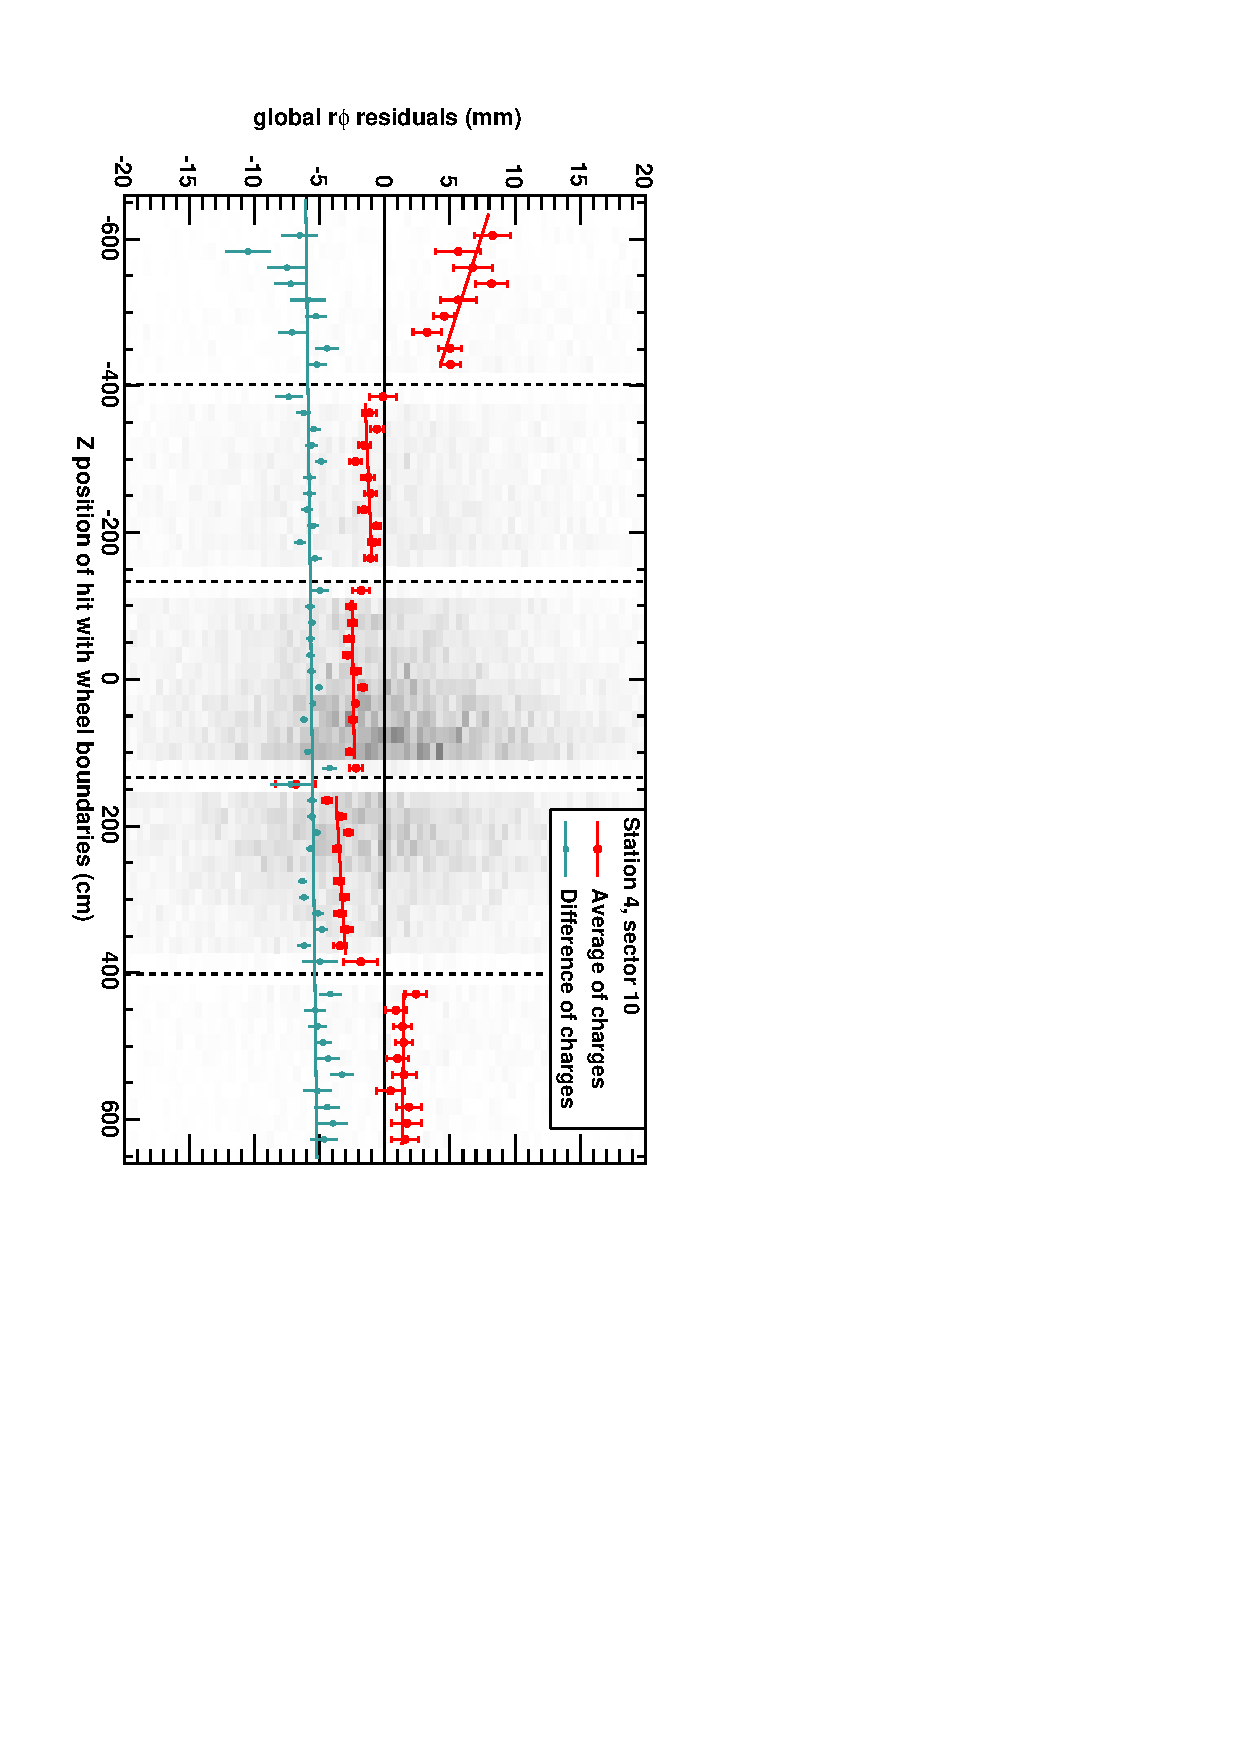
\includegraphics[height=\linewidth, angle=90]{demo_of_bfield.pdf}

\scriptsize grey background is the raw 2-D residuals distribution

linear fits are only a guide for the eye: not used in alignment!
\end{frame}

\begin{frame}
\frametitle{Insensitivity to $\Delta \vec{B}(\vec{x})$}
\begin{itemize}
\item $\vec{B}(\vec{x})$ simulation improved by increasing TOSCA grid volume
\begin{itemize}
\item main problem was not missing material (e.g.\ green structure)
\item simulation's universe was too small: field lines were cramped
\item better but not perfect agreement with tracks and Hall probes
\end{itemize}
\item Re-calculate alignment plots to \textcolor{red}{test insensitivity to new map} and \textcolor{blue}{cross-check correctness of new map}
\begin{itemize}
\item left: histogram of bins from the previous plot (for all sectors)
\item right: how each bin changes when new field is applied
\end{itemize}
\end{itemize}

\vspace{-0.3 cm}
\mbox{ } \hfill {\tiny statistical errors in bins are ${\mathcal O}(\mbox{0.5~mm})$}

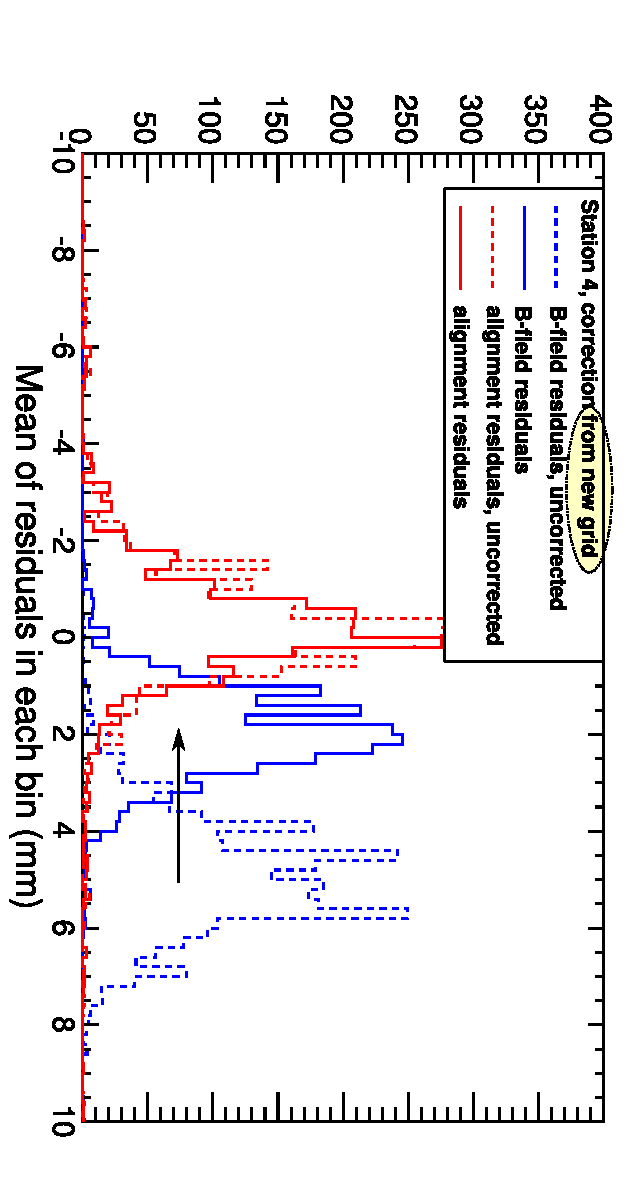
\includegraphics[width=4 cm, angle=90]{newgrid_corrections_station4.pdf} 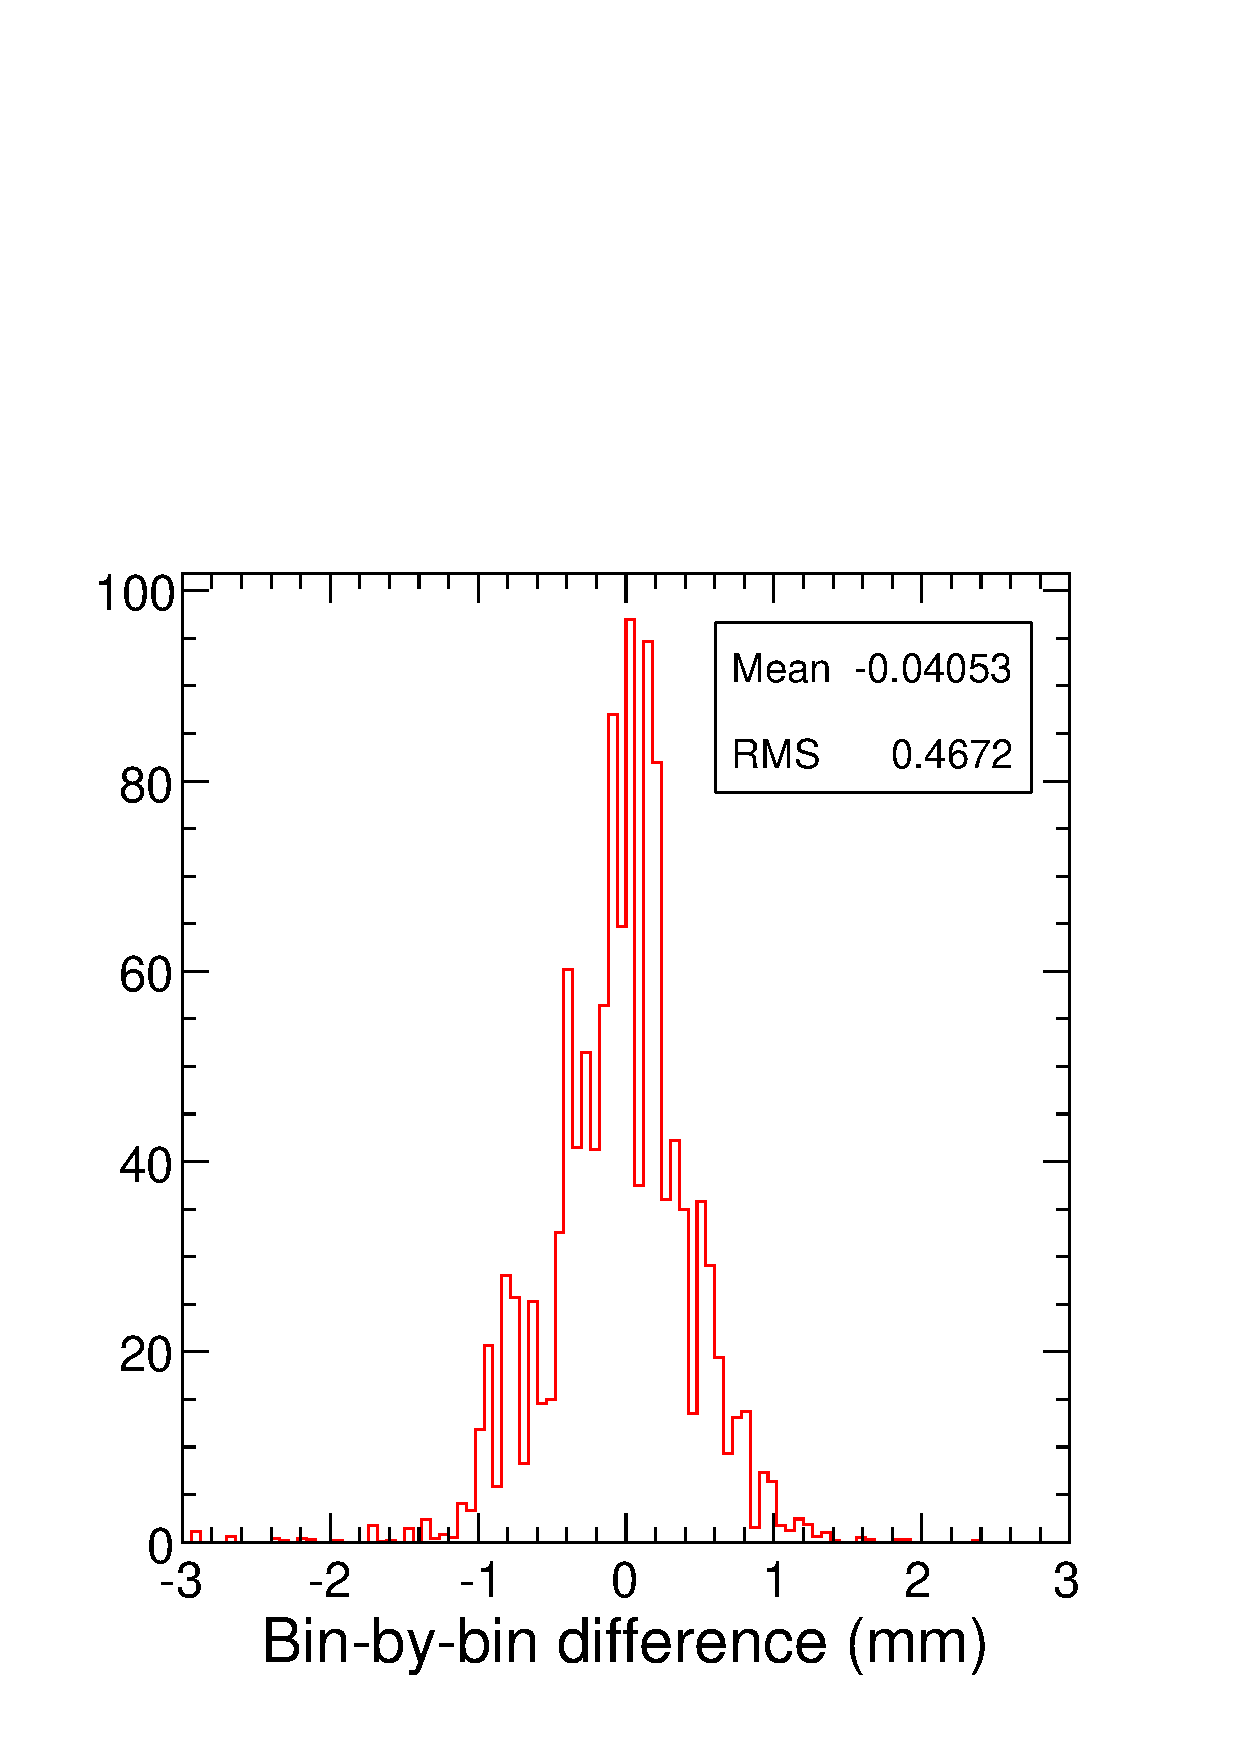
\includegraphics[height=4 cm]{newgrid_binbybin_station4.pdf}
\end{frame}

\begin{frame}
\frametitle{Residuals and {\it single} scattering}

\begin{columns}
\column{0.65\linewidth}

\begin{itemize}
\item Single scattering process has a power-law distribution, while multiple scattering and experimental resolution are Gaussian

\item Peak of residuals distribution should not be computed from
  the mean: it would be pulled by scattered ``outliers''

\item Model process as Lorentzian-Gaussian convolution (Voigt distribution):
\end{itemize}
\column{0.35\linewidth}
\tiny \textcolor{darkblue}{barrel data}

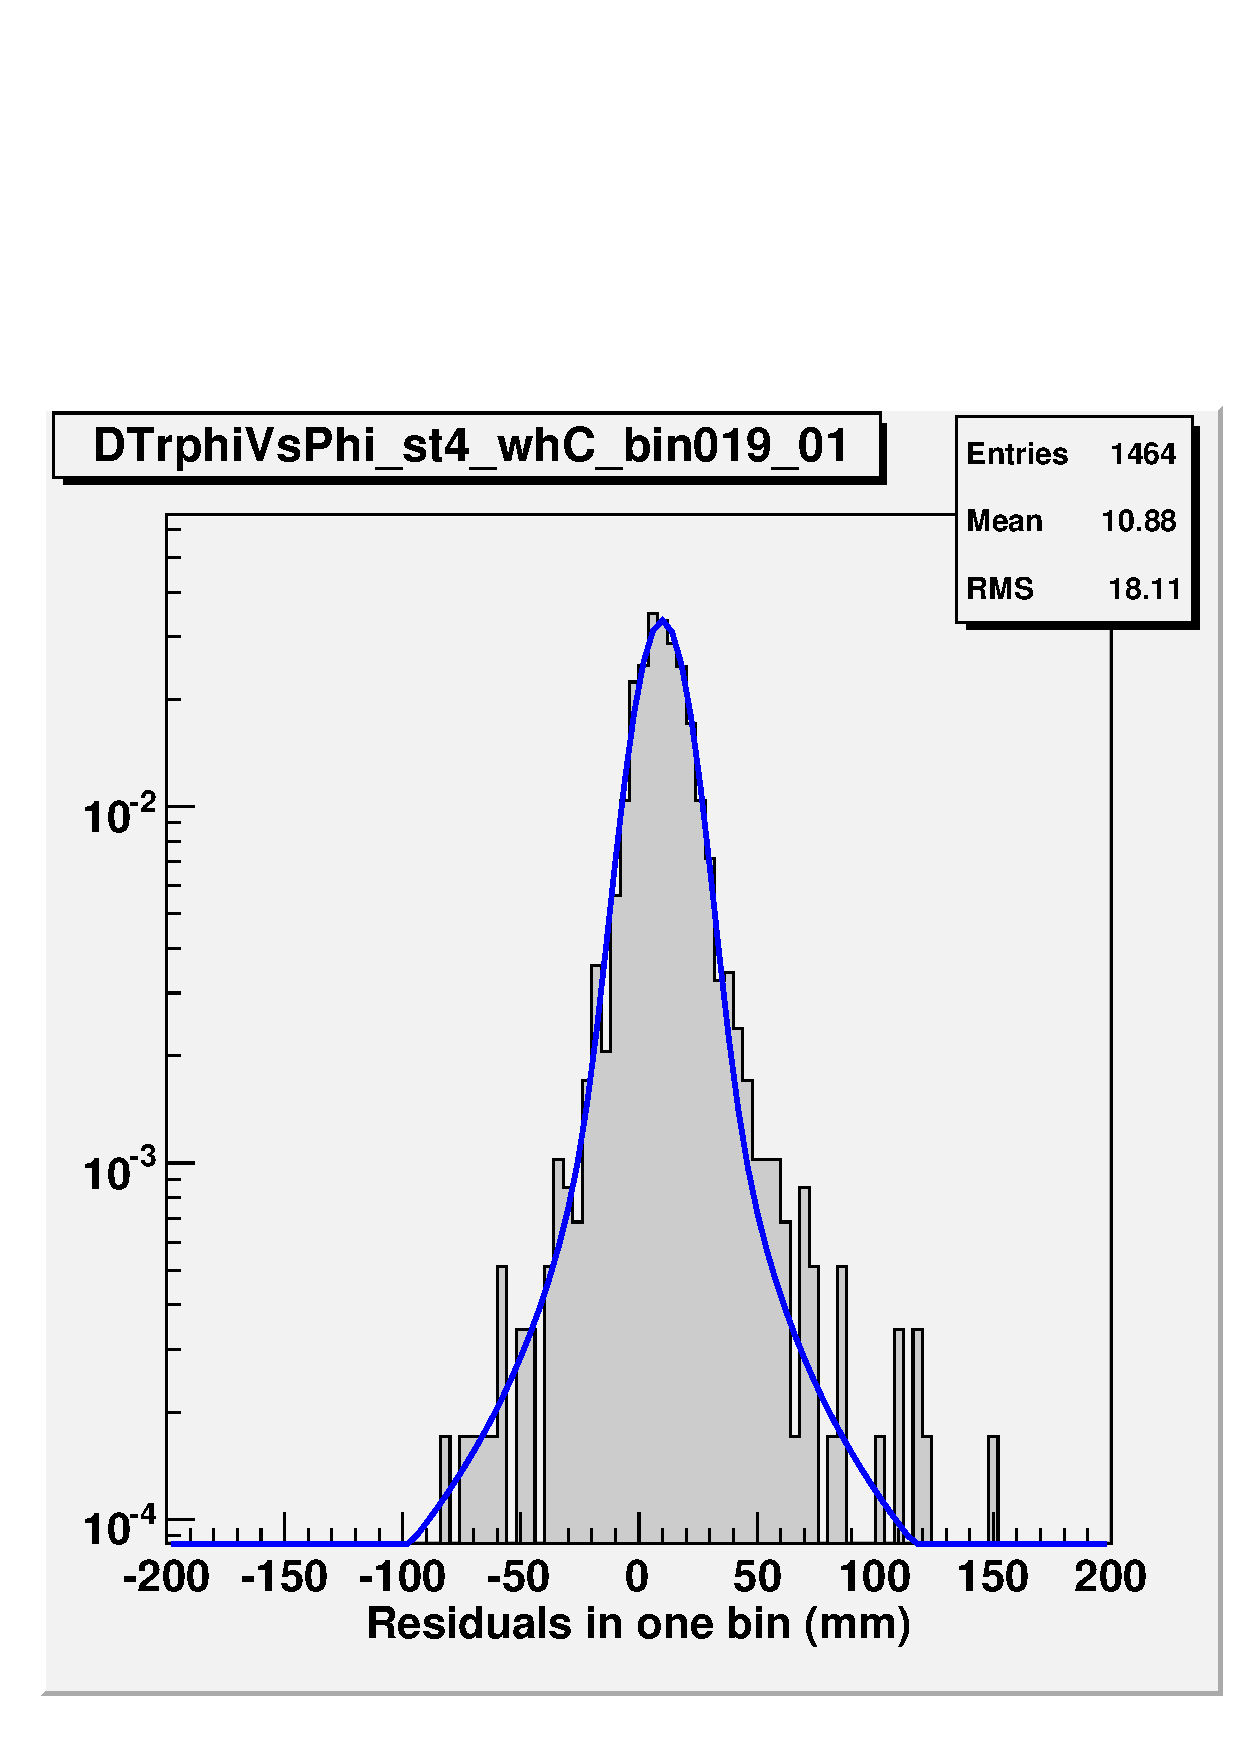
\includegraphics[width=\linewidth]{fitfunction.pdf}
\end{columns}

\vspace{0.45 cm}
\[ f(x) = \int_{-\infty}^\infty \frac{1}{\pi}\frac{\Gamma/2}{(x - \xi - \textcolor{darkblue}{x_0})^2 + (\Gamma/2)^2} \times 
\frac{1}{\sqrt{2\pi} \sigma} \exp\left(\frac{-\xi^2}{2 \sigma^2}\right) \, d\xi \]

\vspace{0.15 cm}
\hspace{-0.45 cm}
\begin{minipage}{\linewidth}
\begin{itemize}
\item Determine peak (alignment correction) from $\textcolor{darkblue}{x_0}$ of unbinned fit
\begin{itemize}\setlength{\itemsep}{0.1 cm}
\item regular mean ($\sum x_i/N$) = center of an unbinned Gaussian fit
\item this is the same thing, but with tails
\item ``outliers'' contribute far less to $f(x)$ log-likelihood \mbox{than Gaussian\hspace{-1 cm}}
\end{itemize}
\end{itemize}
\end{minipage}
\end{frame}

\begin{frame}
\frametitle{Fitting more parameters}

\begin{columns}
\column{0.5\linewidth}
\begin{itemize}
\item Center of peak = translation
\item Rotations and out-of-plane translations introduce linear trends in residuals
\end{itemize}

\vspace{0.2 cm}
\column{0.5\linewidth}

\vspace{0.2 cm}
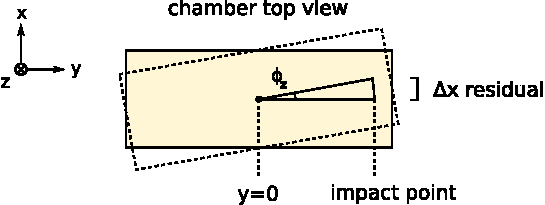
\includegraphics[width=\linewidth]{phiz_diagram.pdf}
\end{columns}

\begin{columns}
\column{0.5\linewidth}
\tiny \textcolor{darkblue}{endcap Monte Carlo}

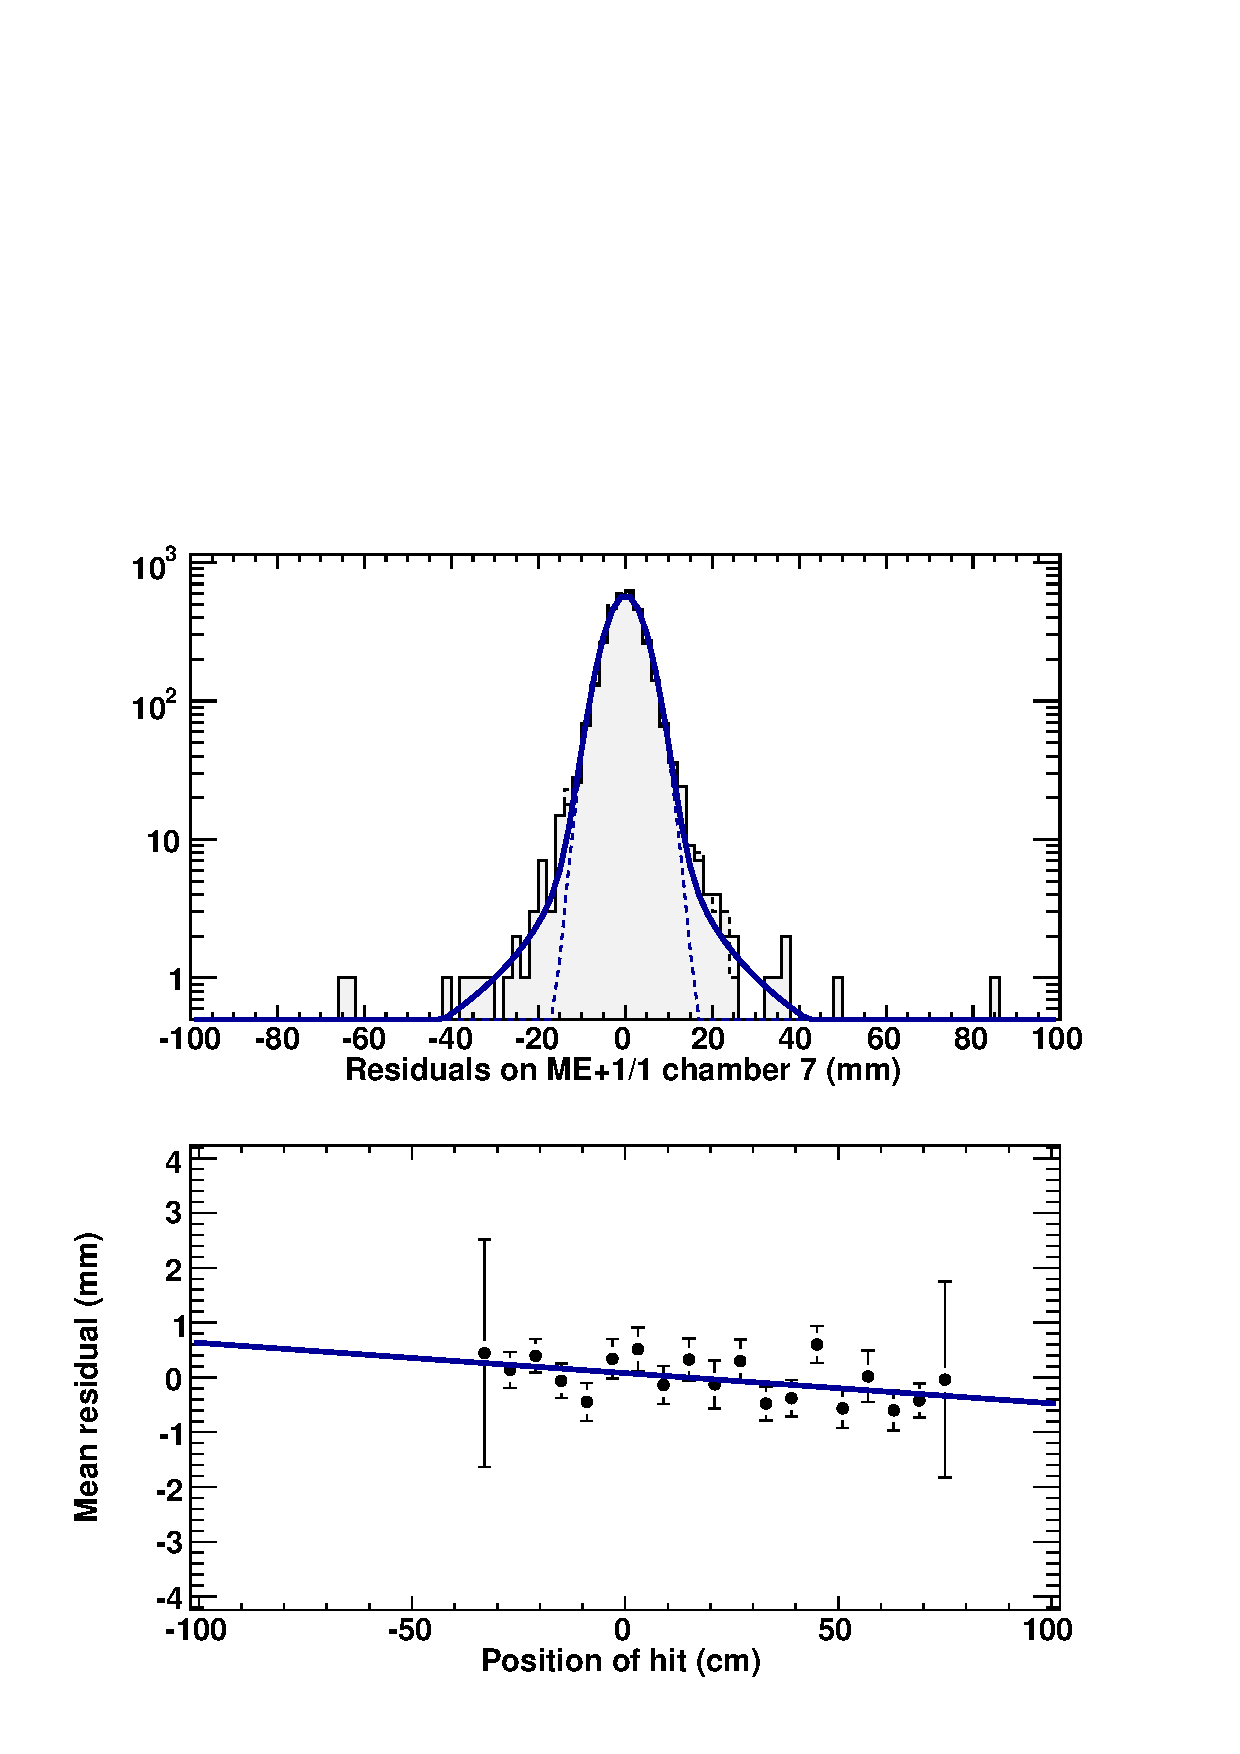
\includegraphics[width=\linewidth]{phizfit_demo_MEp11_7.pdf}
\column{0.5\linewidth}
\mbox{ } \hfill 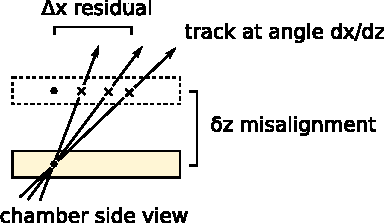
\includegraphics[width=0.8\linewidth]{zpos_diagram.pdf} \hfill \mbox{ }

\vspace{0.25 cm}
\begin{itemize}
\item Determine multiple parameters from simultaneous fit:

\textcolor{darkblue}{``$x_0$''} $\to$ \textcolor{darkblue}{$\delta x$} $+$ \textcolor{darkblue}{$\phi_z$} $y$ $+$ \textcolor{darkblue}{$\delta z$} $\dfrac{dx}{dz}$

\item Consistent treatment that's easy to diagnose with plots
\end{itemize}
\end{columns}
\end{frame}

\begin{frame}
\frametitle{Is it a real alignment?}
\label{page:rphivsphi}

\hspace{-0.3 cm}
\begin{minipage}{\linewidth}
\begin{columns}
\column{0.5\linewidth}
\begin{itemize}
\item We want to find the real positions of chambers, not just minimize residuals
\item To look for biases in the track source, plot residuals \mbox{more finely\hspace{-0.5 cm}} than the chamber boundaries
\begin{itemize}
\item bias can change residuals shape inside chambers and across boundaries
\item only misalignments can make discontinuities at chamber boundaries
\end{itemize}
\item Cause of linear slopes in \mbox{$r\phi$ vs.\ $\phi$\hspace{-0.5 cm}} (bottom) under investigation {\scriptsize (DTs stretched in $x$?  tested $\phi_y$ and $z$-shift hypotheses\ldots)}

\item \mbox{Complete set of plots: \textcolor{blue}{\tt \tiny \href{http://indico.cern.ch/conferenceDisplay.py?confId=51267}{http://indico.cern.ch/conferenceDisplay.py?confId=51267}} \tiny (``more information'')\hspace{-10 cm}}
\end{itemize}

\column{0.6\linewidth}

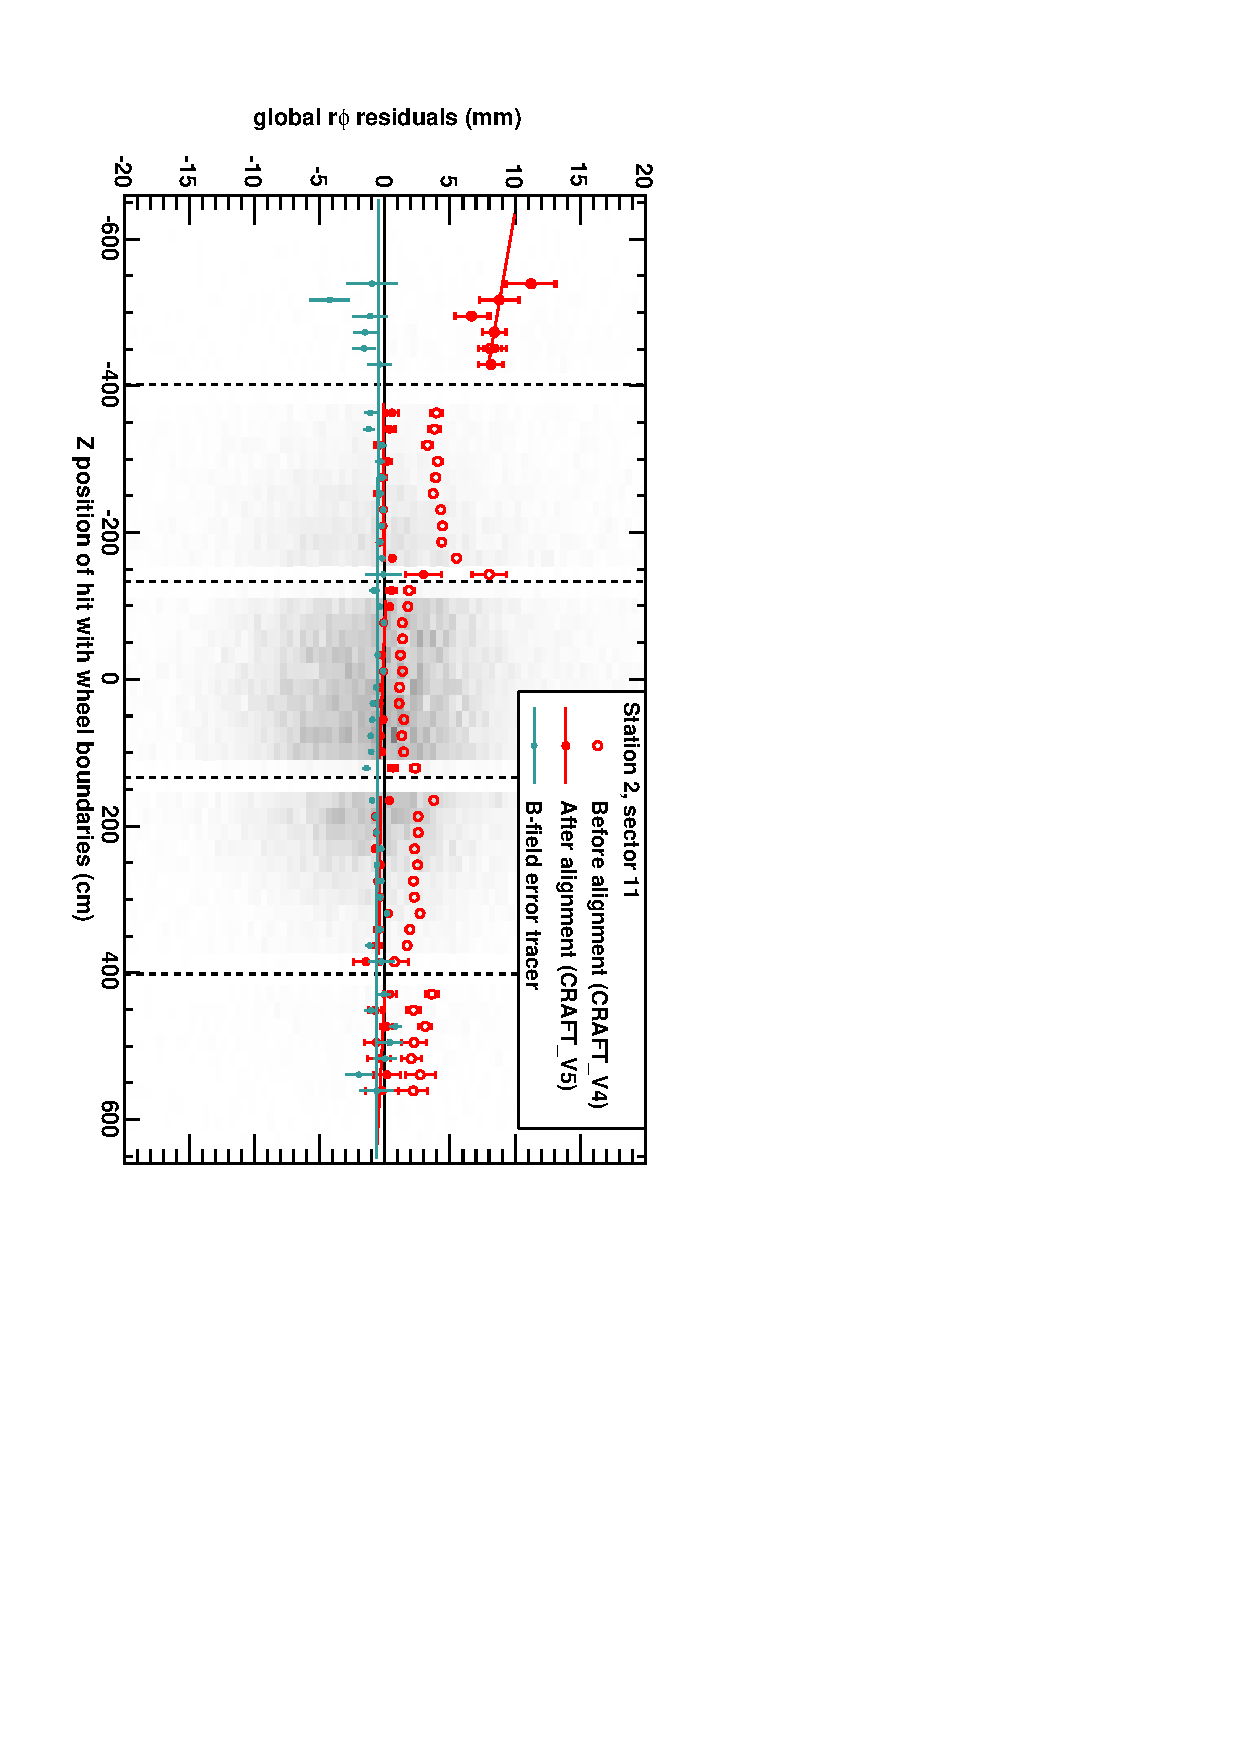
\includegraphics[height=1.1\linewidth, angle=90]{alignmentplots_example1.pdf}

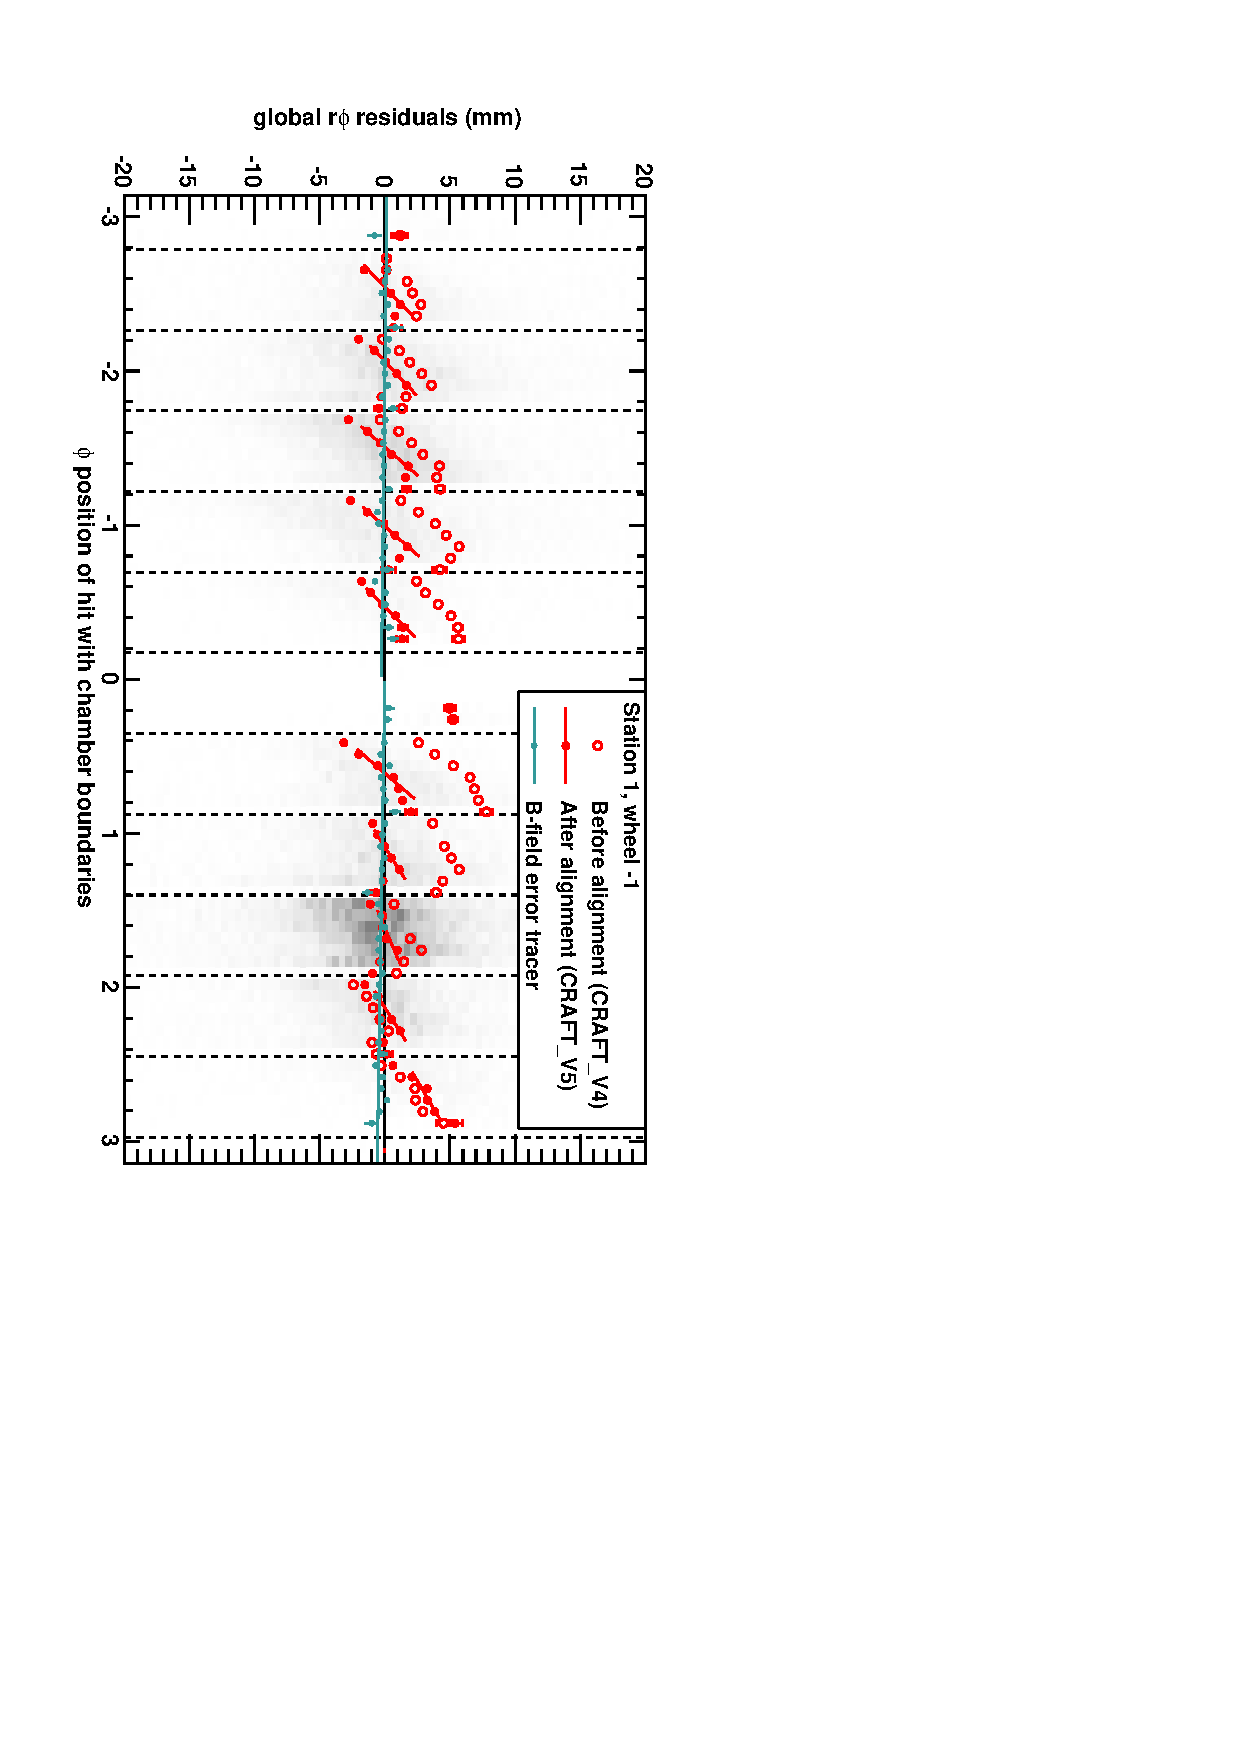
\includegraphics[height=1.1\linewidth, angle=90]{alignmentplots_example2.pdf}

\vspace{0.3 cm}
\end{columns}
\end{minipage}
\end{frame}

\begin{frame}
\frametitle{Same thing for the endcaps}

\begin{minipage}{\linewidth}
\begin{columns}
\column{0.4\linewidth}

\begin{itemize}\setlength{\itemsep}{0.2 cm}
\item Plot CSC residuals vs.\ $R$, rather than $Z$
\begin{itemize}
\item note expected $R^2$ \mbox{resolution dependence\hspace{-1 cm}}
\end{itemize}

\item $\phi$ plots are similar \mbox{to DTs\hspace{-1 cm}}

\vspace{0.2 cm}
\mbox{\hspace{-0.5 cm}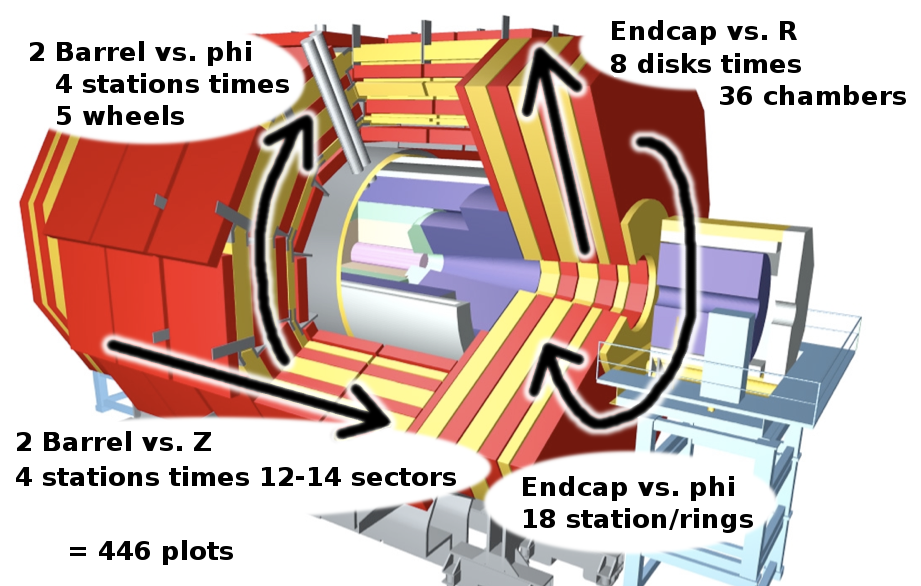
\includegraphics[width=1.3\linewidth]{CMS_cutaway.png}}

\vspace{0.2 cm}
\item Large number of diagnostic plots
\item \mbox{Future: must condense information into a few key validation plots\hspace{-10 cm}}
\end{itemize}

\column{0.6\linewidth}

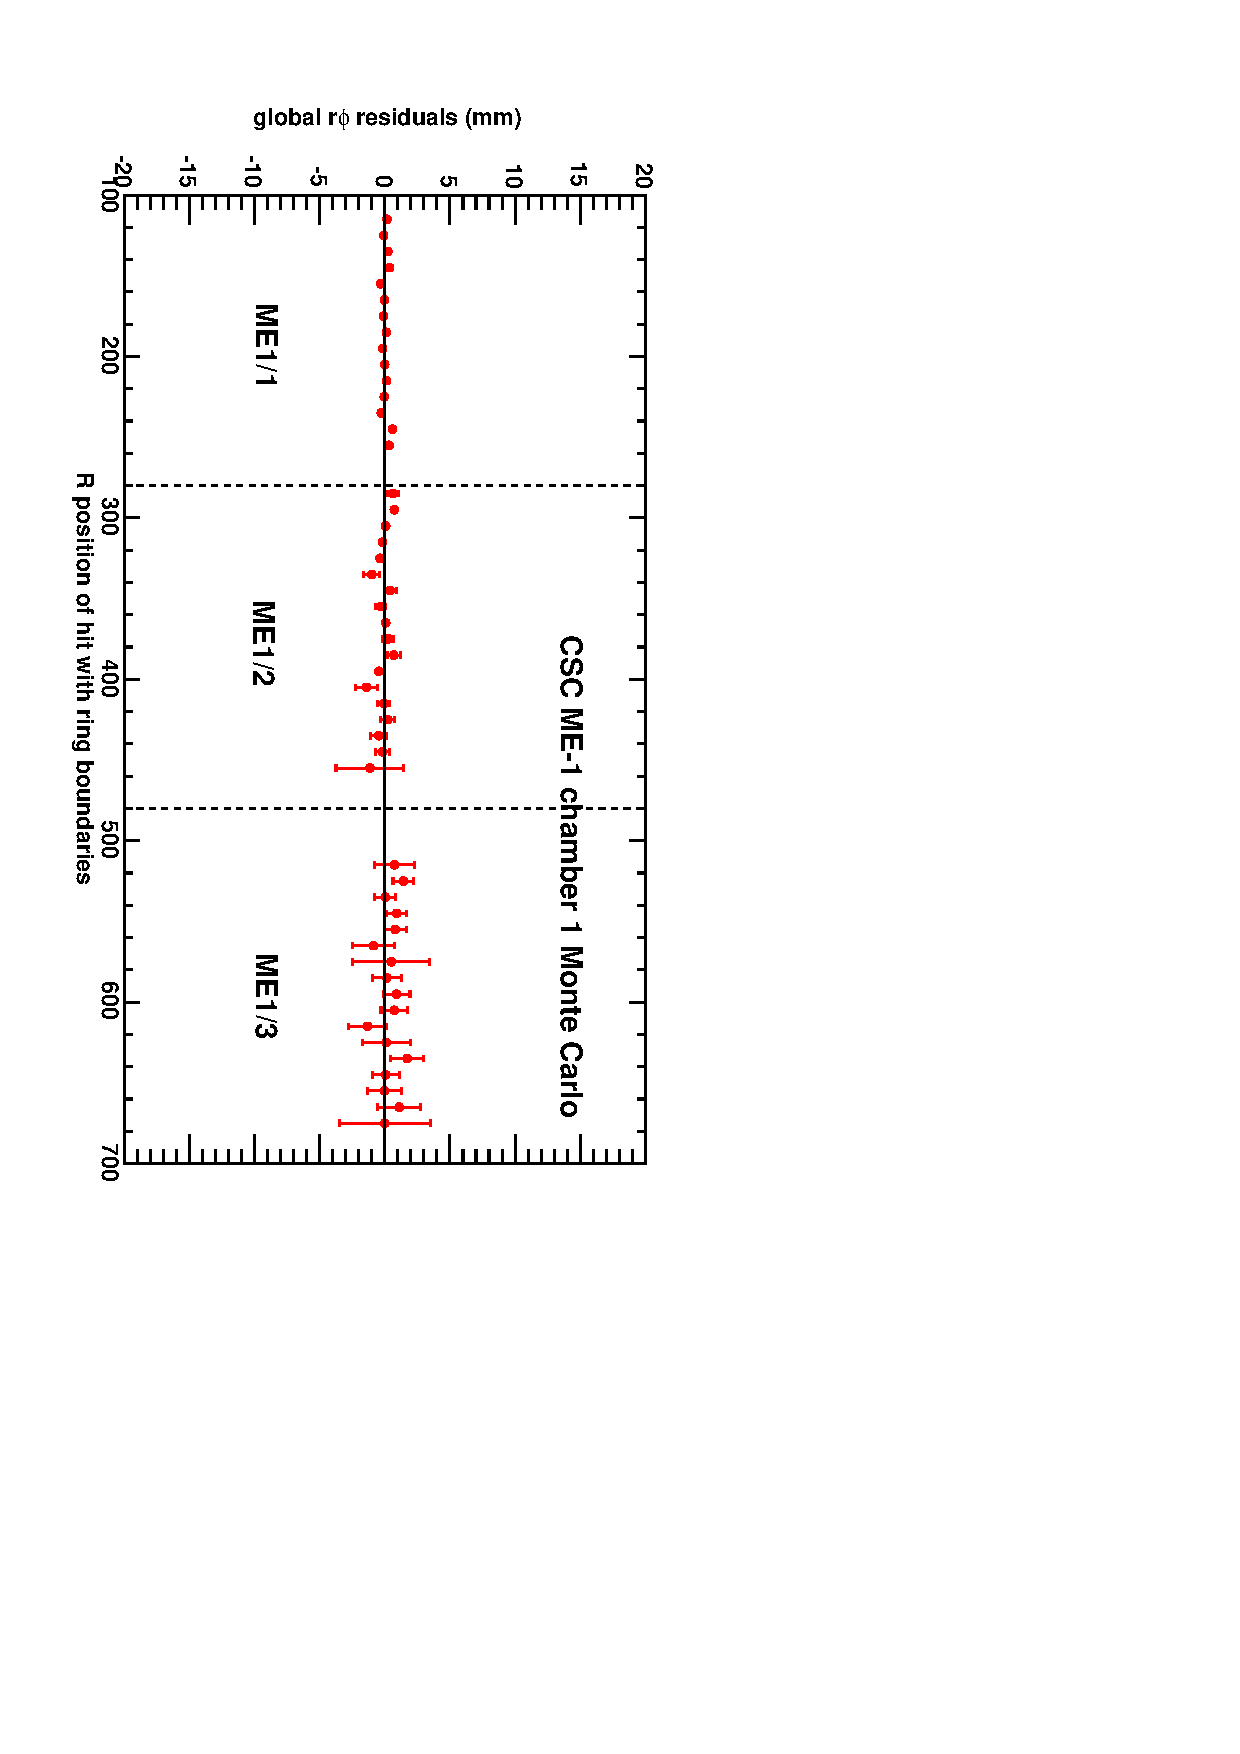
\includegraphics[height=1.1\linewidth, angle=90]{CSCrphires_vsR_MEm1ch01_MC.pdf}

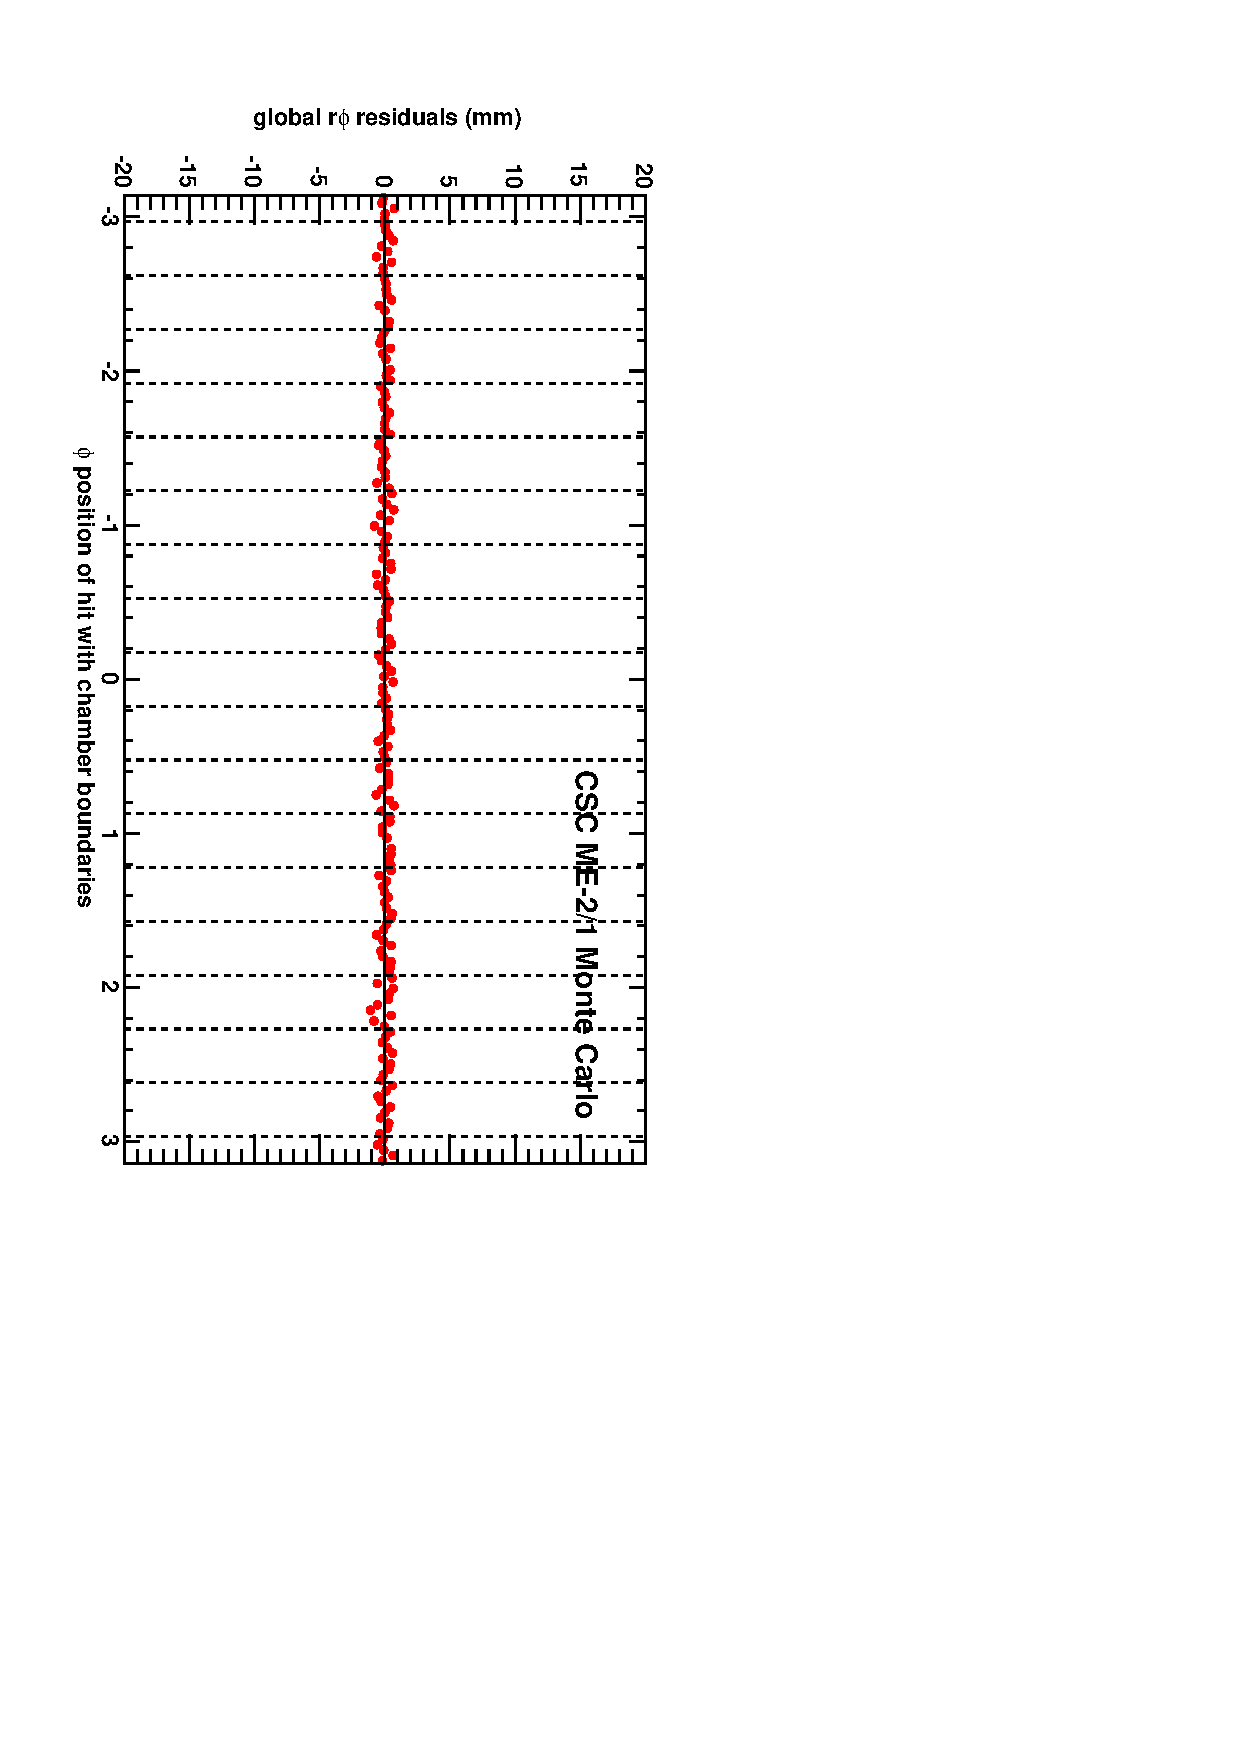
\includegraphics[height=1.1\linewidth, angle=90]{CSCrphires_vsphi_MEm21_MC.pdf}

\vspace{0.3 cm}
\end{columns}
\end{minipage}
\end{frame}

\begin{frame}
\frametitle{Tracker radiography}

\vspace{0.25 cm}
\begin{columns}
\column{0.5\linewidth}
\begin{itemize}
\item Tracker misalignment or weak modes would bias muon alignment
\item Non-projective cosmic rays allow us to investigate\ldots
\end{itemize}

\column{0.5\linewidth}
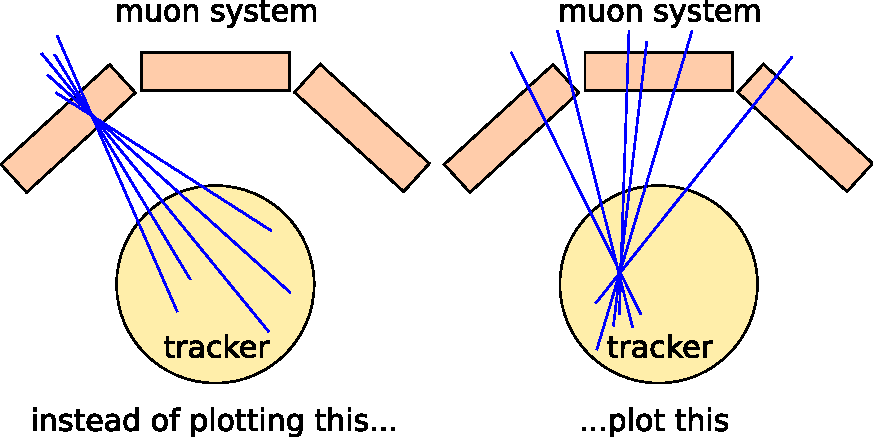
\includegraphics[width=\linewidth]{tracker_xray.pdf}
\end{columns}

\vspace{0.25 cm}
\begin{columns}
\column{0.5\linewidth}

observation of TEC $z$ misalignment {\scriptsize (CRAFT\_V4, not latest constants)}

\mbox{ } \hfill 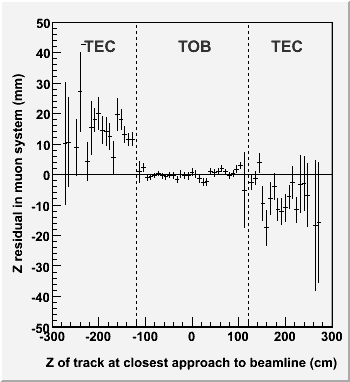
\includegraphics[width=0.7\linewidth]{zresid_from_tracker_outerbottom.png} \hfill \mbox{ }

\column{0.5\linewidth}

sensitivity study, tracker twist added by hand \textcolor{blue}{(blue)}

\mbox{ } \hfill 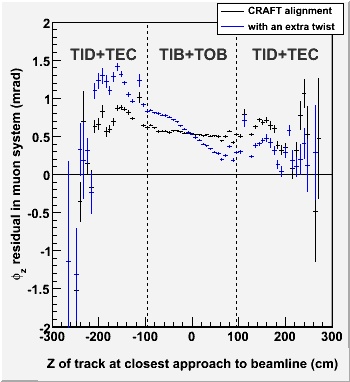
\includegraphics[width=0.7\linewidth]{phiresid_from_tracker_inner_twist2.png} \hfill \mbox{ }

\end{columns}
\end{frame}

\begin{frame}
\frametitle{Barrel alignment results}

\begin{itemize}
\item The following are alignment corrections used in \mbox{CRAFT re-processing\hspace{-1 cm}}
\begin{itemize}
\item local $x$ is in the $r\phi$ direction, local $y$ is along the beamline
\item $x$ re-expressed as $\phi$ to demonstrate \mbox{lack of wheel rotations\hspace{-1 cm}}
\end{itemize}
\end{itemize}

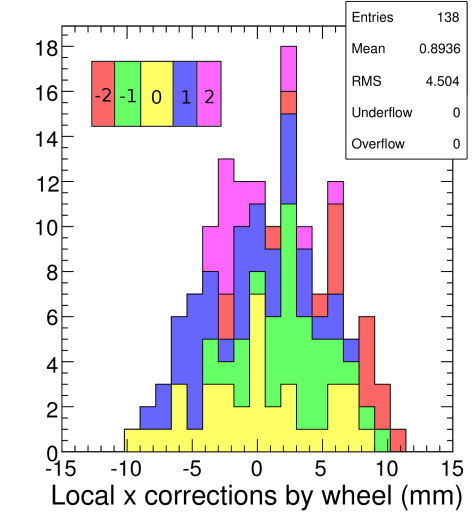
\includegraphics[width=0.25\linewidth]{report2_xbywheel.png} 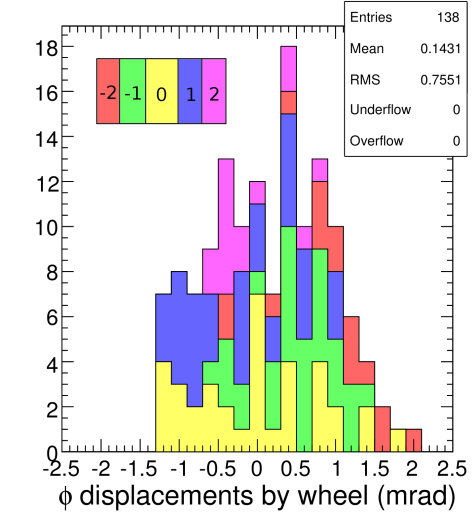
\includegraphics[width=0.25\linewidth]{report2_phibywheel.png} 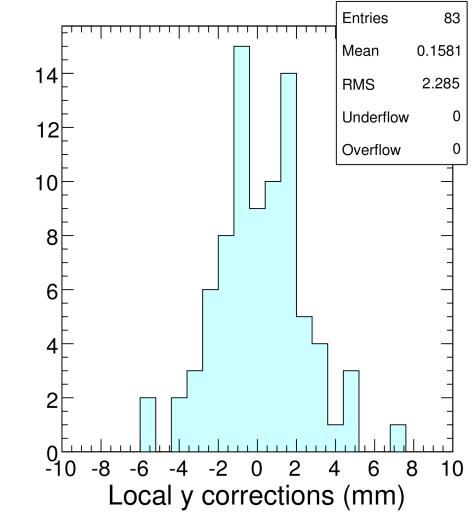
\includegraphics[width=0.25\linewidth]{report2_y.png} 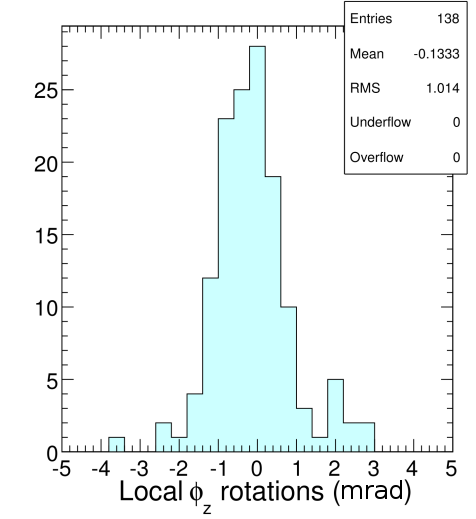
\includegraphics[width=0.25\linewidth]{report2_phiz.png}

\begin{center}
\begin{tabular}{c c}
\textcolor{red}{aligned} in local $x$ and $\phi_z$: & \textcolor{red}{aligned} in local $y$: \\
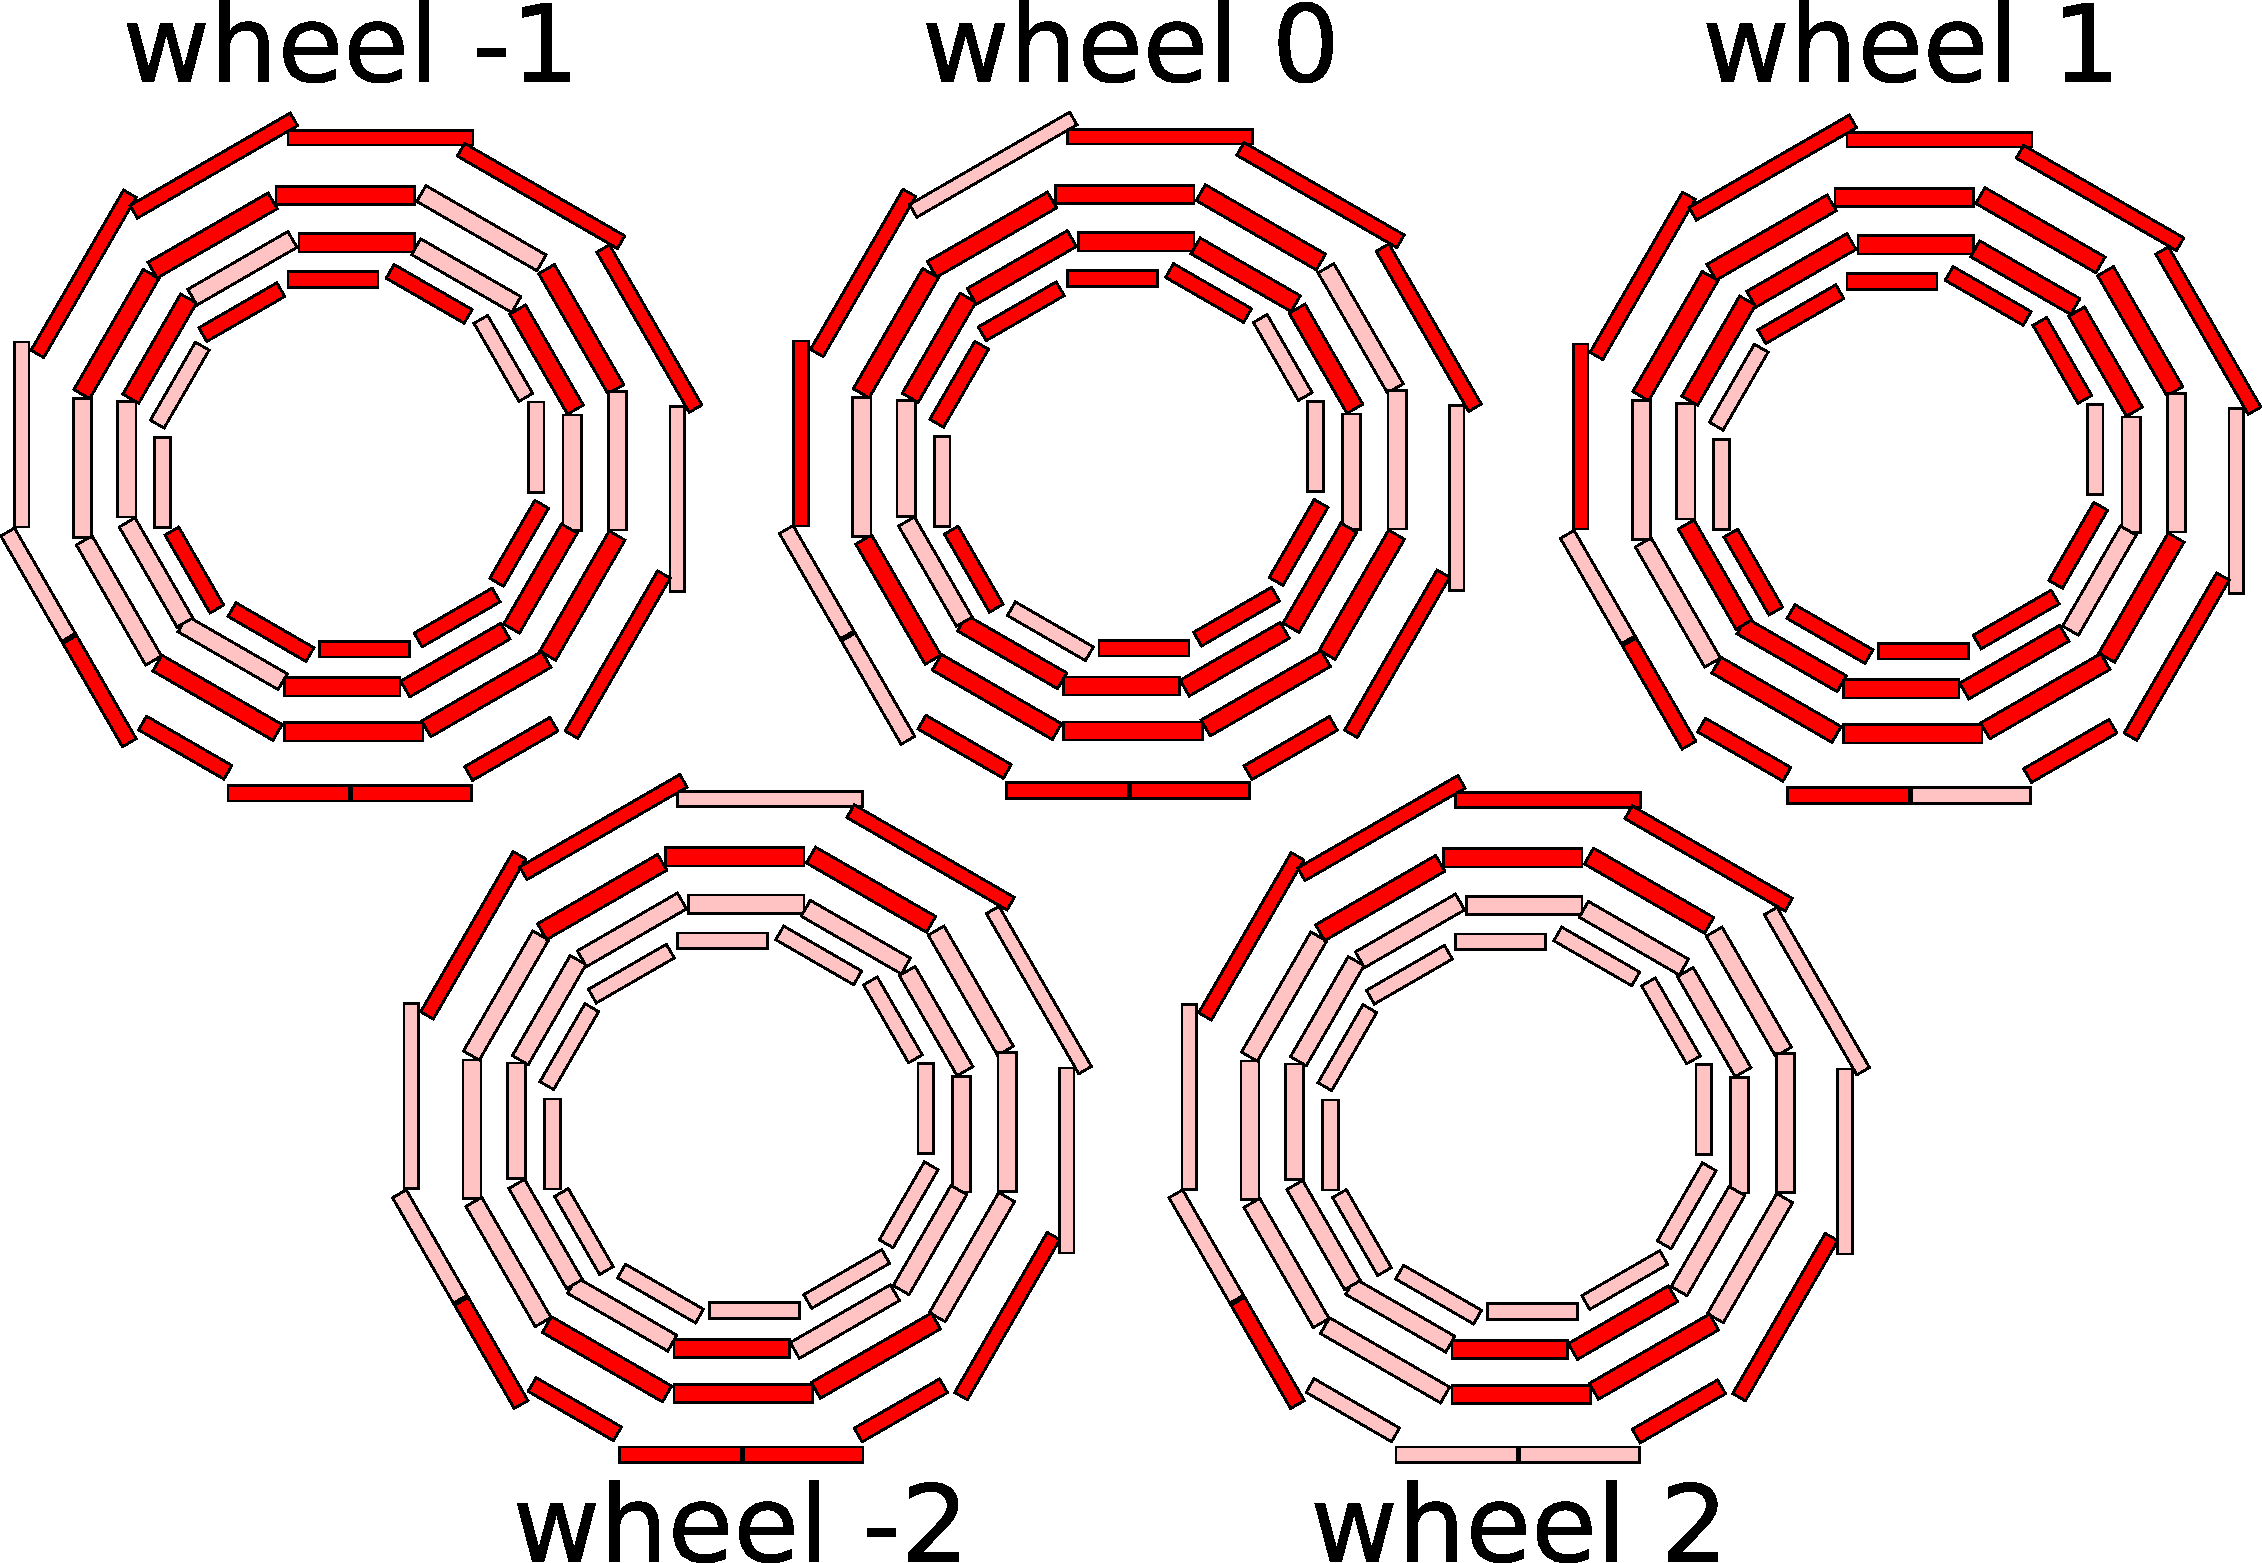
\includegraphics[width=0.4\linewidth]{aligned_rphi.pdf} & 
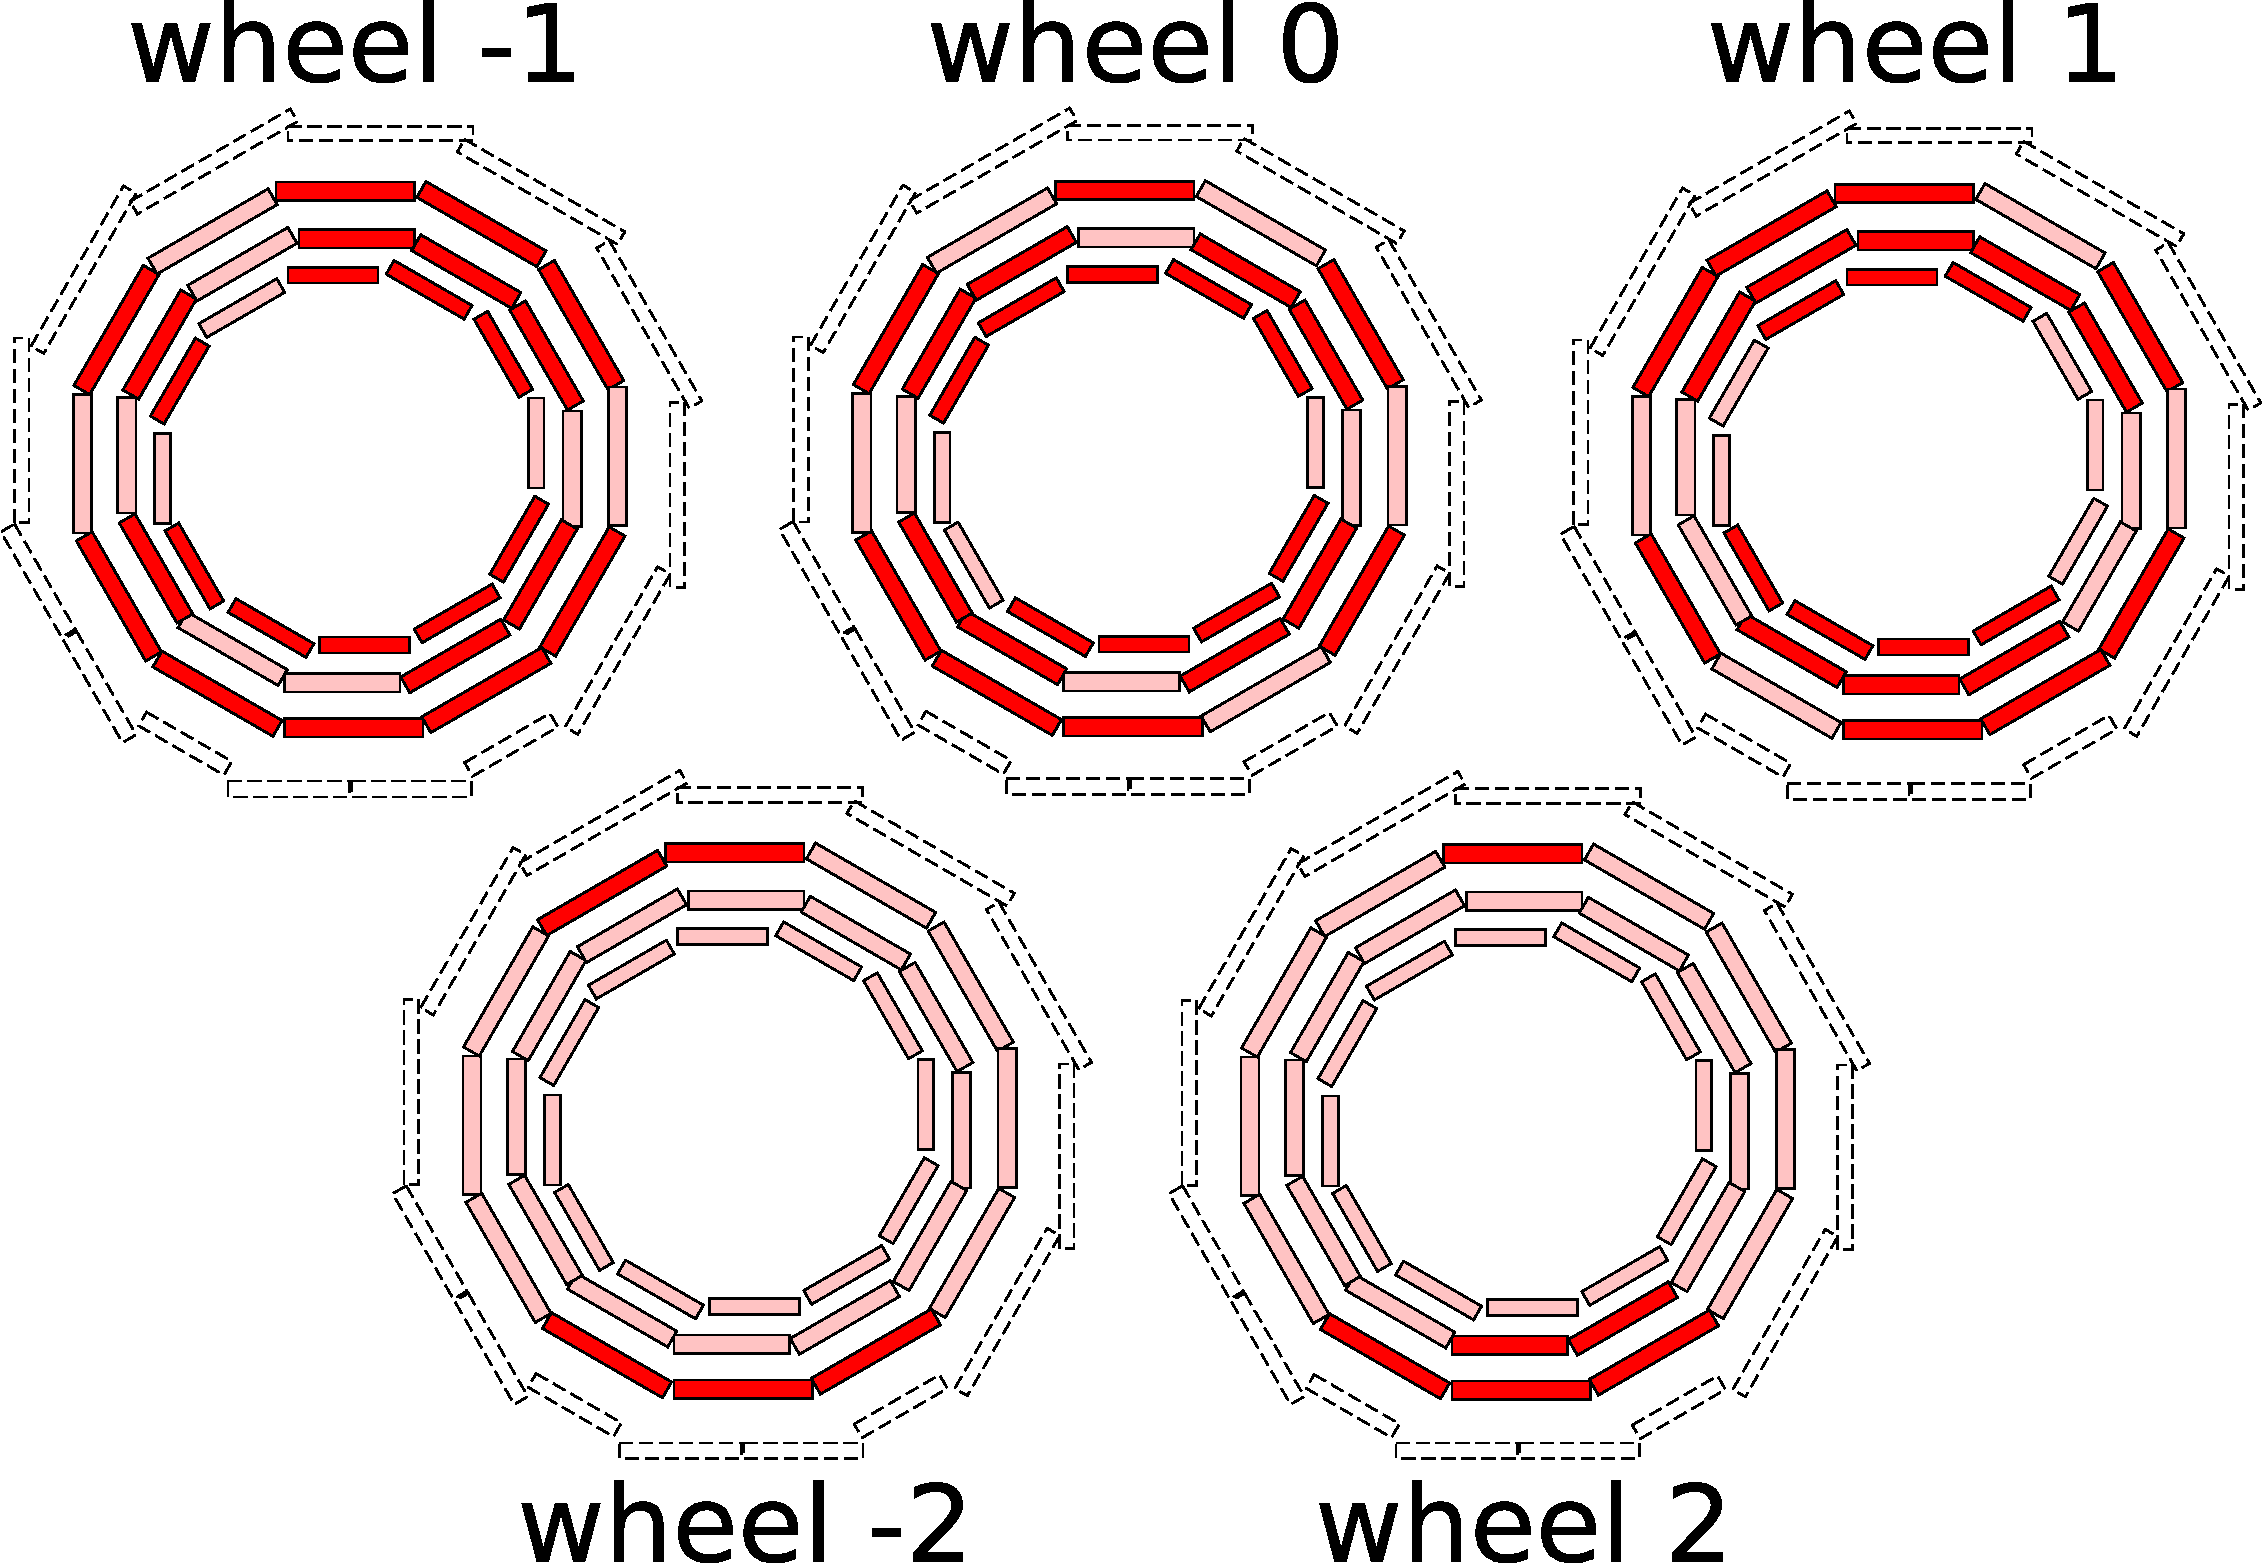
\includegraphics[width=0.4\linewidth]{aligned_z.pdf}
\end{tabular}
\end{center}
\end{frame}

\begin{frame}
\frametitle{Cross-check: relative positions}

\begin{itemize}\setlength{\itemsep}{0.1 cm}
\item Alignment procedure determines chamber positions \mbox{relative to tracker\hspace{-1 cm}}
\item Chamber positions relative to other chambers is a true cross-check
\item Difference of residuals on the same track uses the track as a
  curved ruler to compare two chambers:

\mbox{ } \hfill \mbox{$\mbox{difference} = \big(\mbox{st.\ 3 track} - \mbox{st.\ 3 hit}\big) - \big(\mbox{st.\ 2 track} - \mbox{st.\ 2 hit}\big)$} \hfill \mbox{ }
\end{itemize}

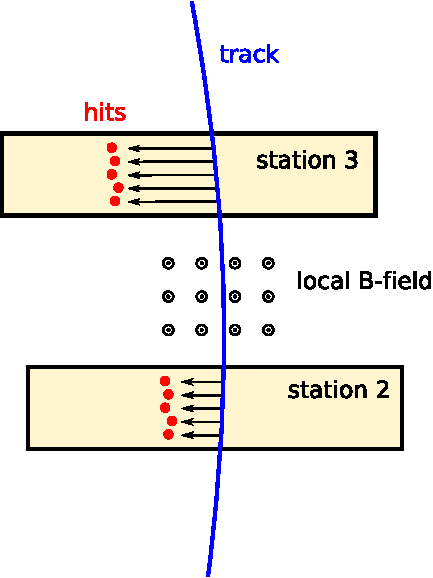
\includegraphics[height=4.4 cm]{residuals_difference.pdf} 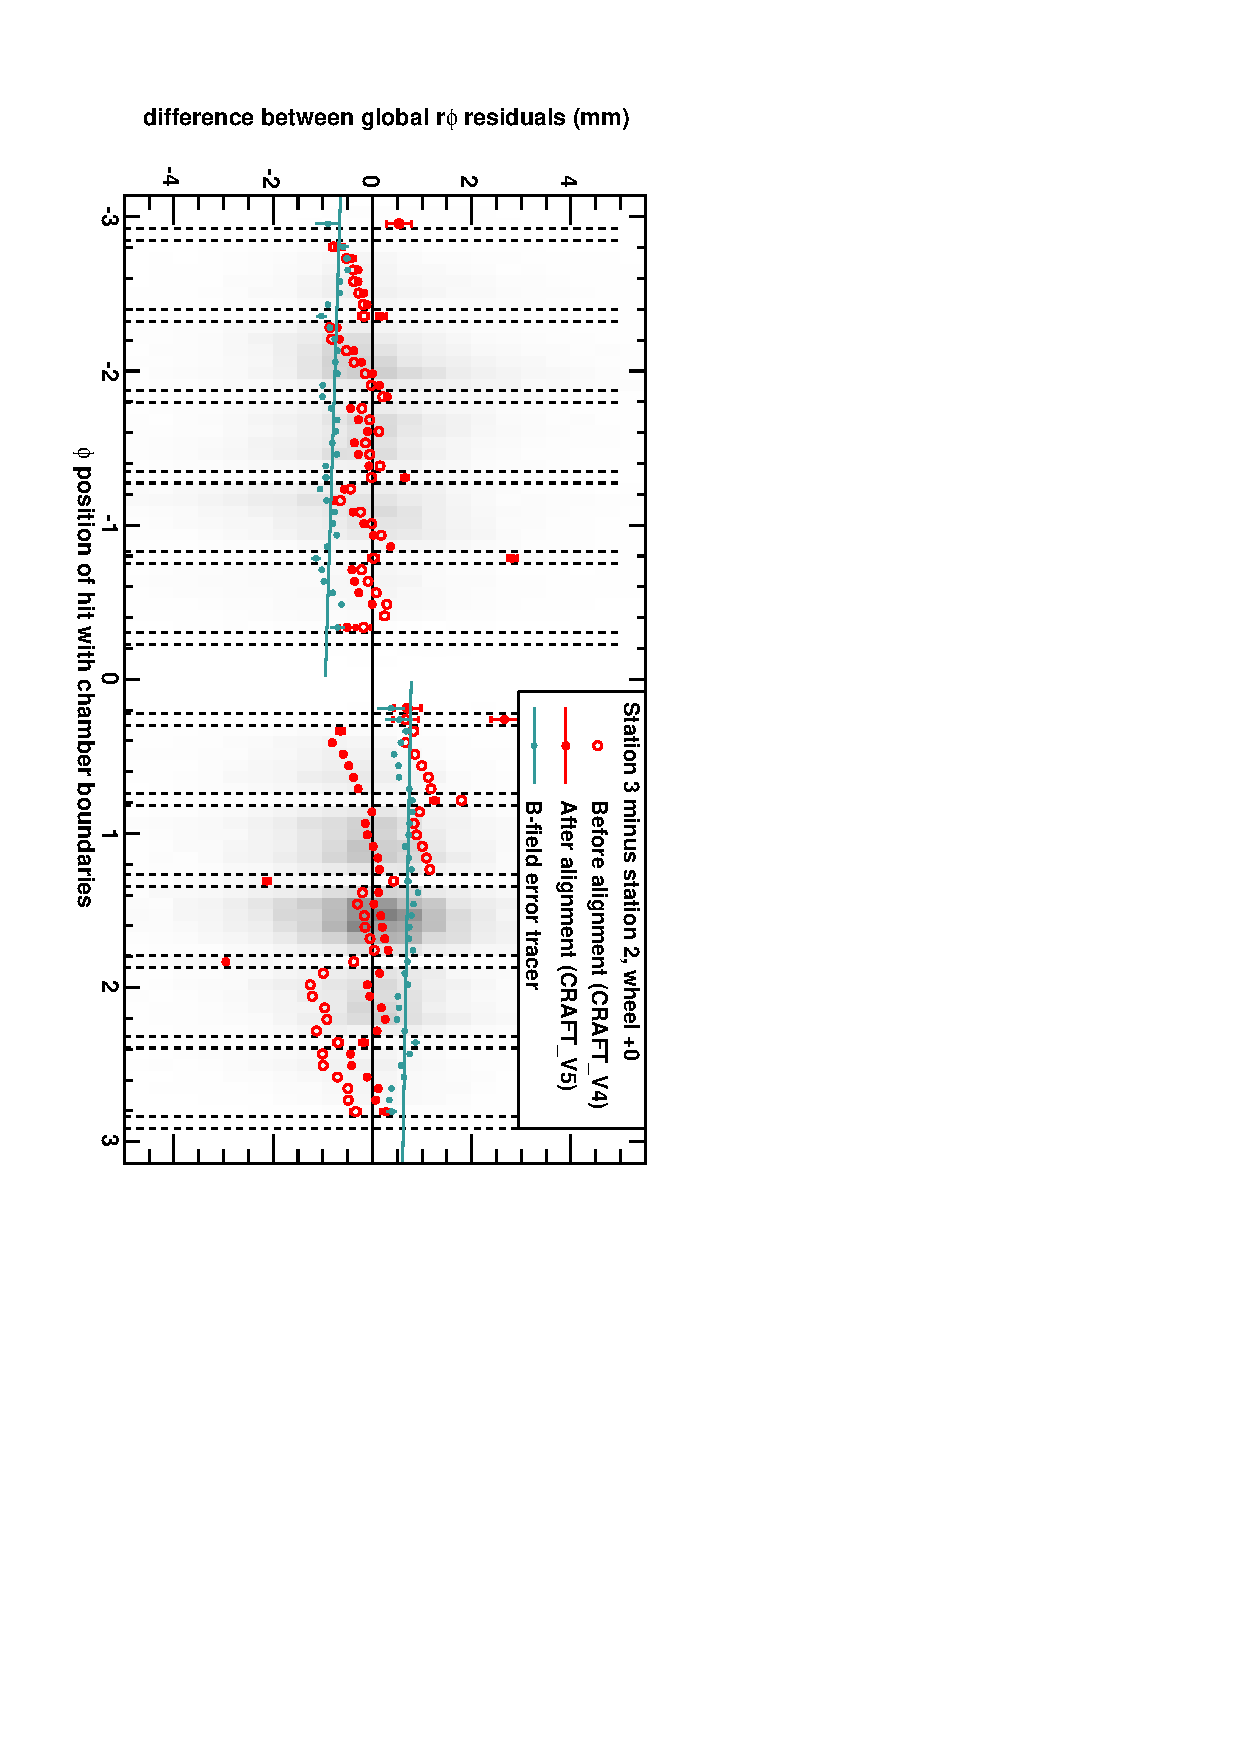
\includegraphics[width=4.5 cm, angle=90]{alignmentplots_example4.pdf}

\begin{itemize}
\item Difference distributions are about 4 times narrower than residuals
\end{itemize}
\end{frame}

\begin{frame}
\frametitle{Residuals after barrel alignment}

\begin{itemize}
\item Alignment narrowed and centered residuals distributions, as it must
\end{itemize}

\vspace{-0.2 cm}
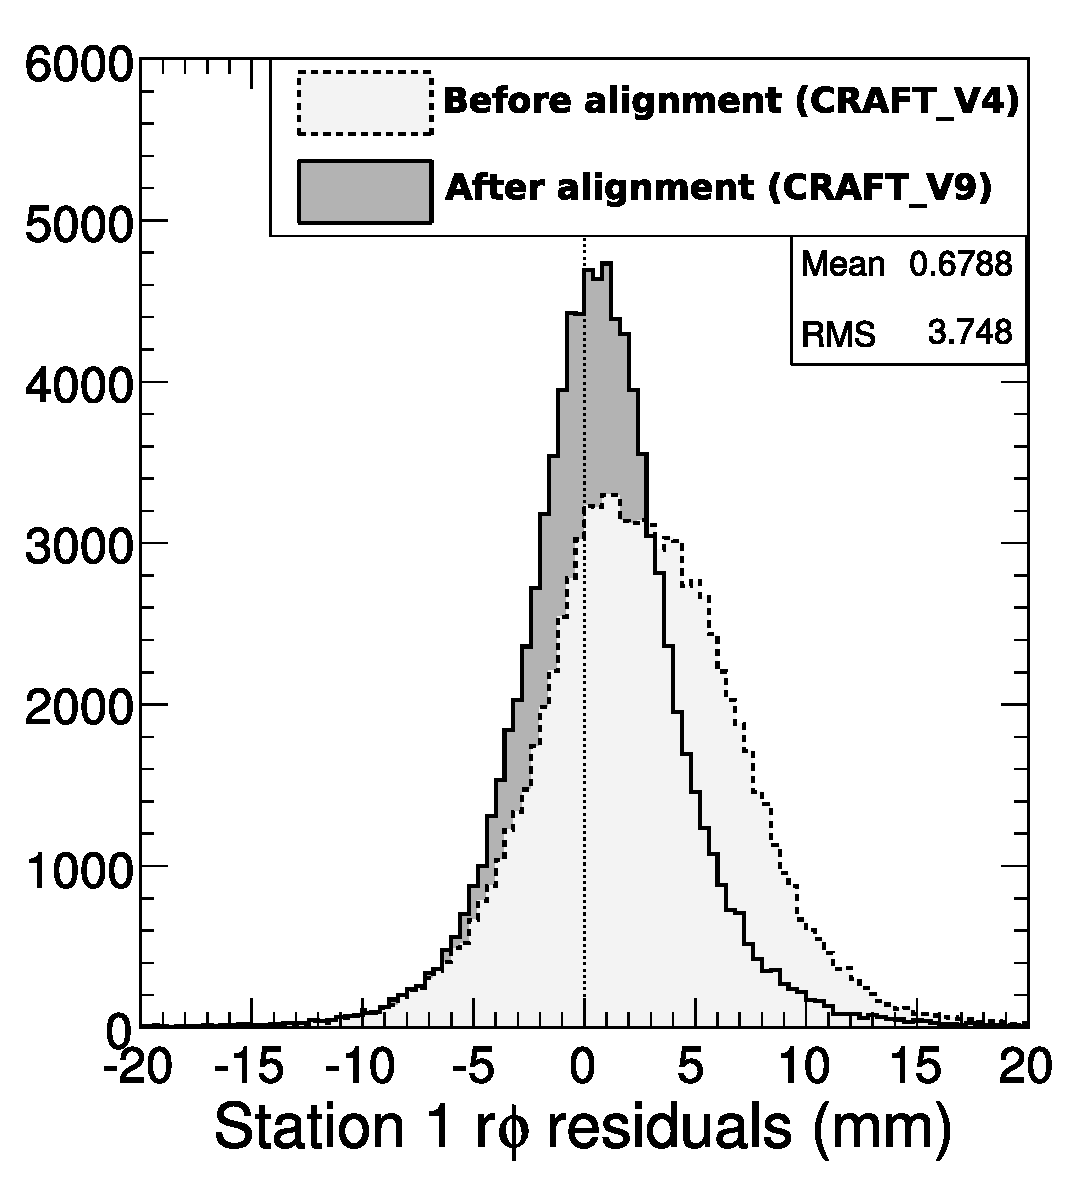
\includegraphics[width=0.25\linewidth]{residuals_improvement1_relabled.pdf} 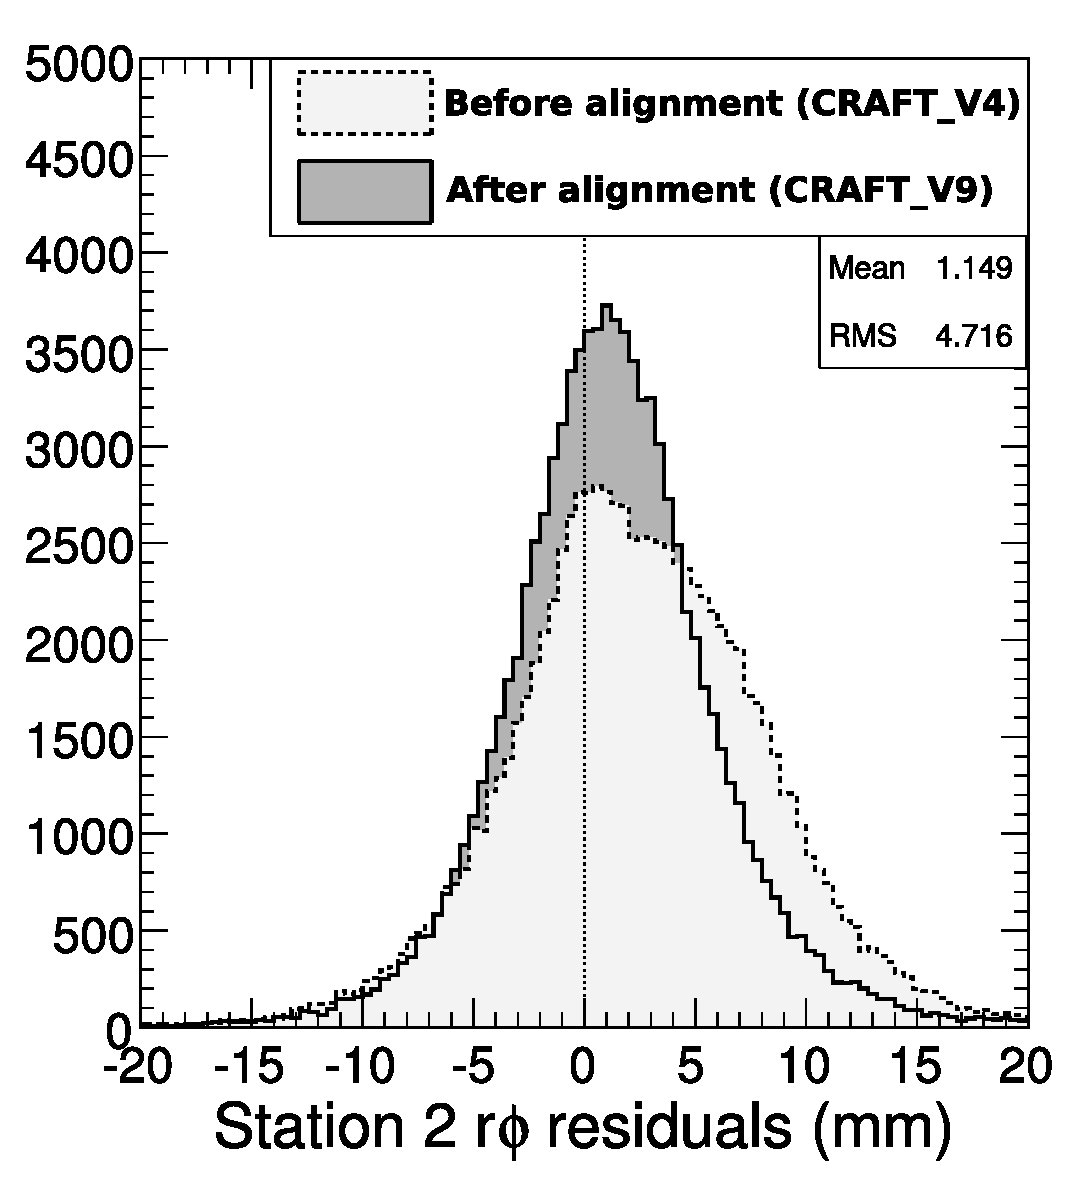
\includegraphics[width=0.25\linewidth]{residuals_improvement2_relabled.pdf} 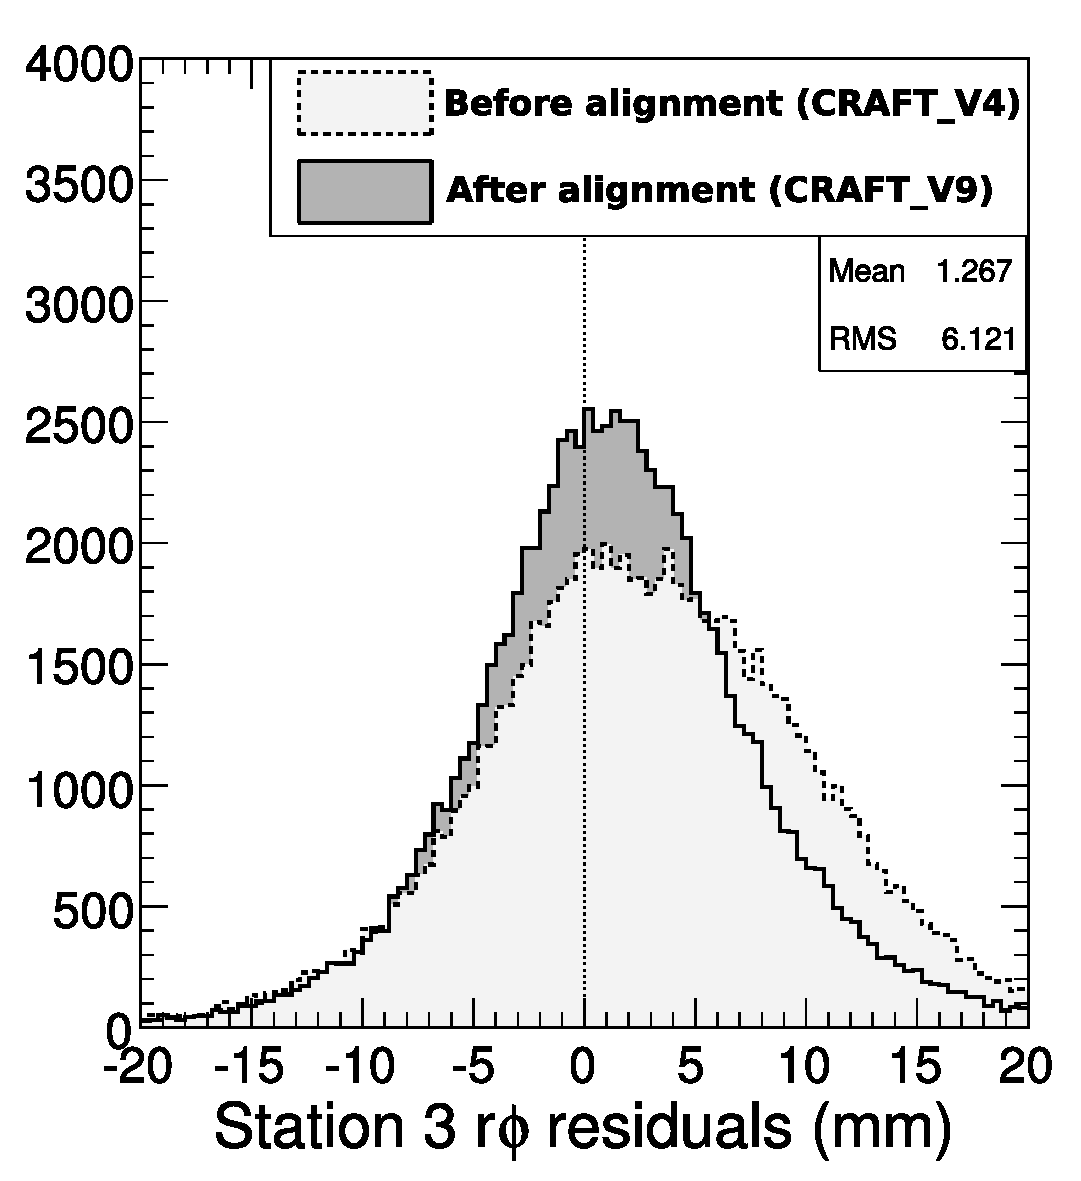
\includegraphics[width=0.25\linewidth]{residuals_improvement3_relabled.pdf} 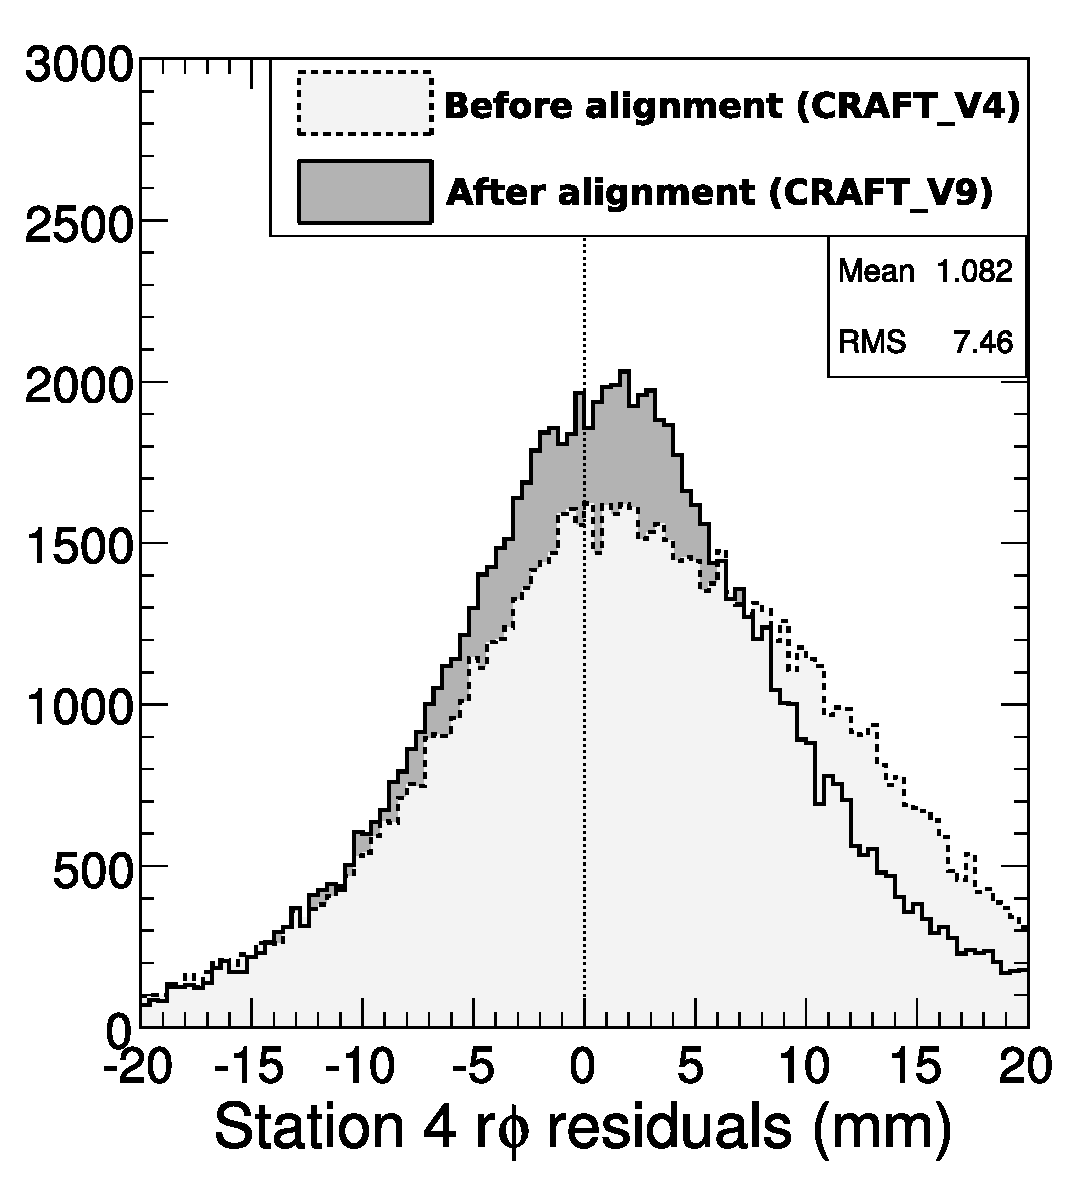
\includegraphics[width=0.25\linewidth]{residuals_improvement4_relabled.pdf}

\begin{itemize}
\item Alignment preserved but didn't improve \mbox{residuals differences\hspace{-1 cm}}
\begin{itemize}
\item 1--2~mm {\it relative} chamber positions before and after alignment
\end{itemize}
\end{itemize}

\vspace{-0.2 cm}
\mbox{ } \hfill 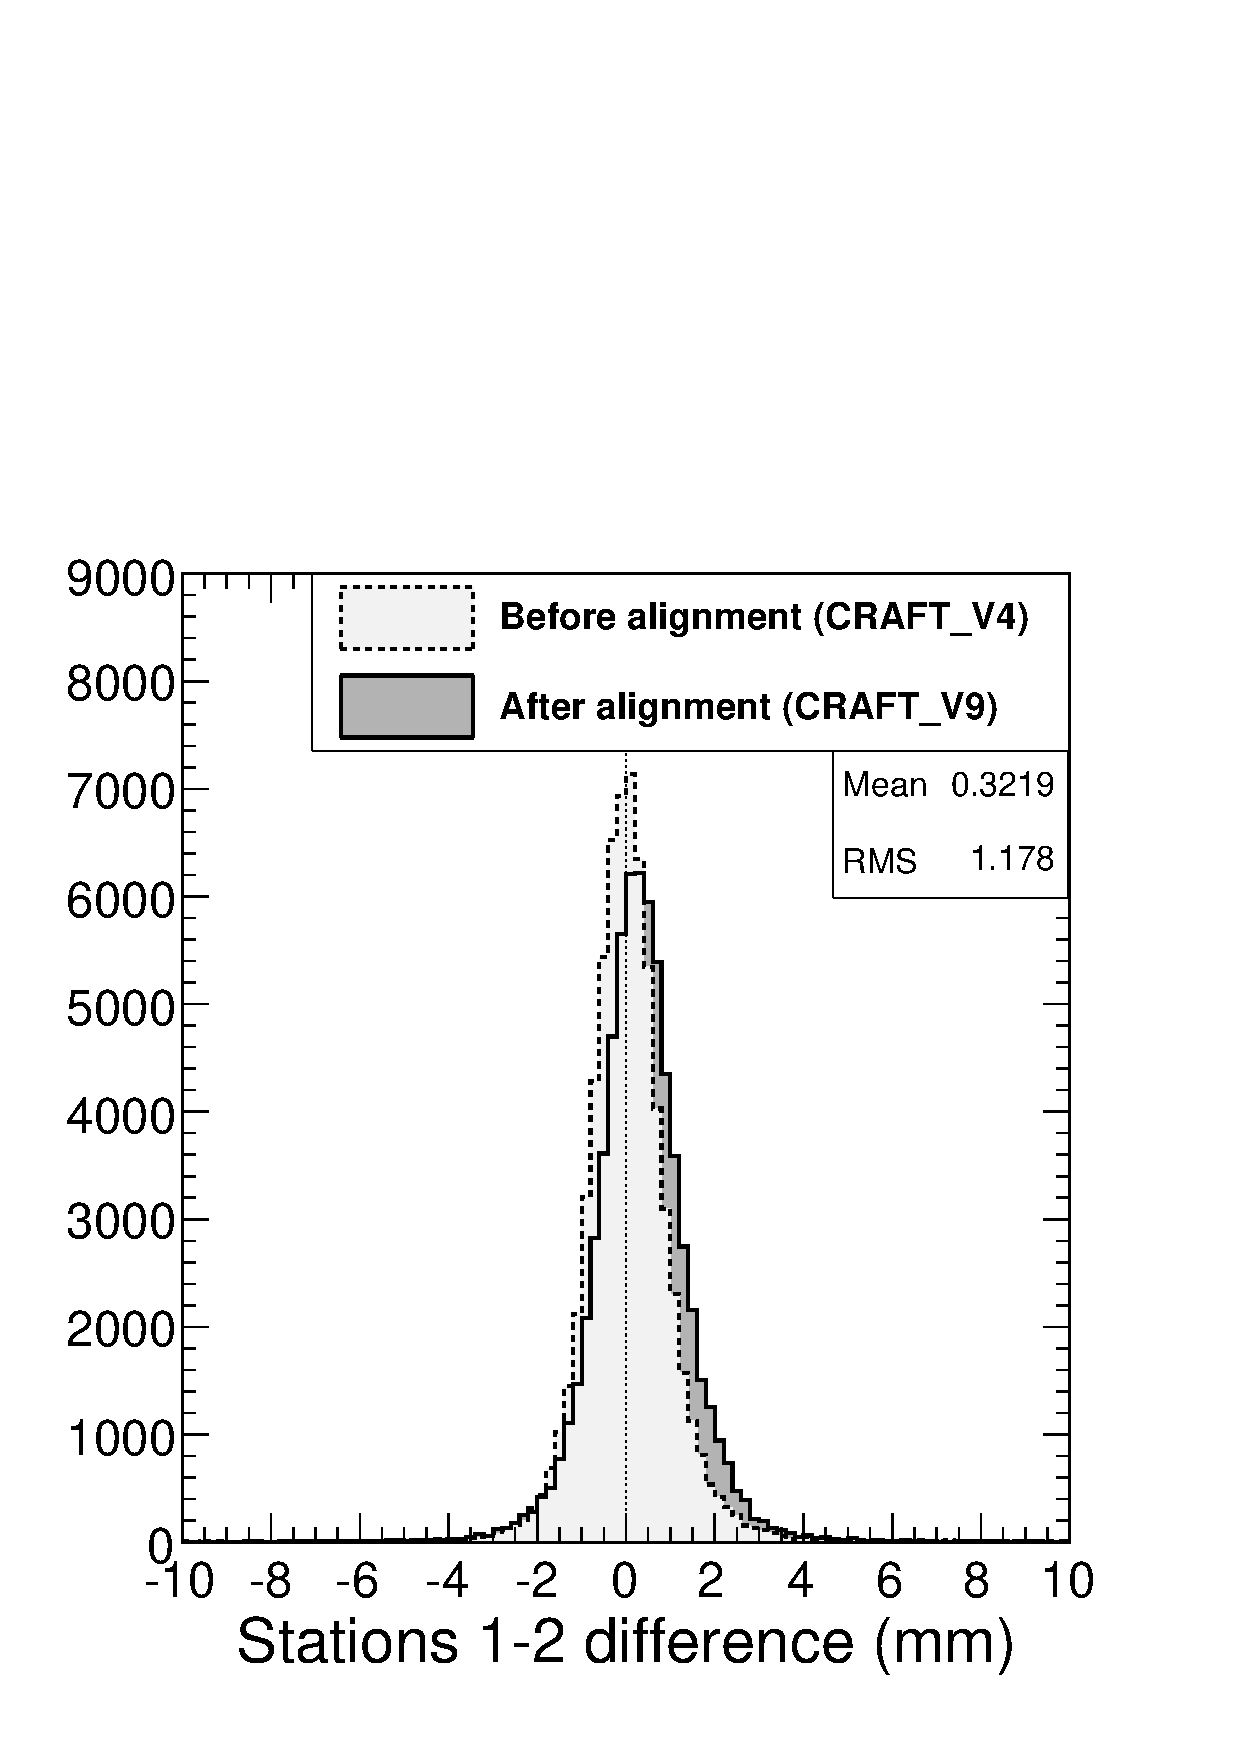
\includegraphics[width=0.25\linewidth]{residdiff12.pdf} \hfill 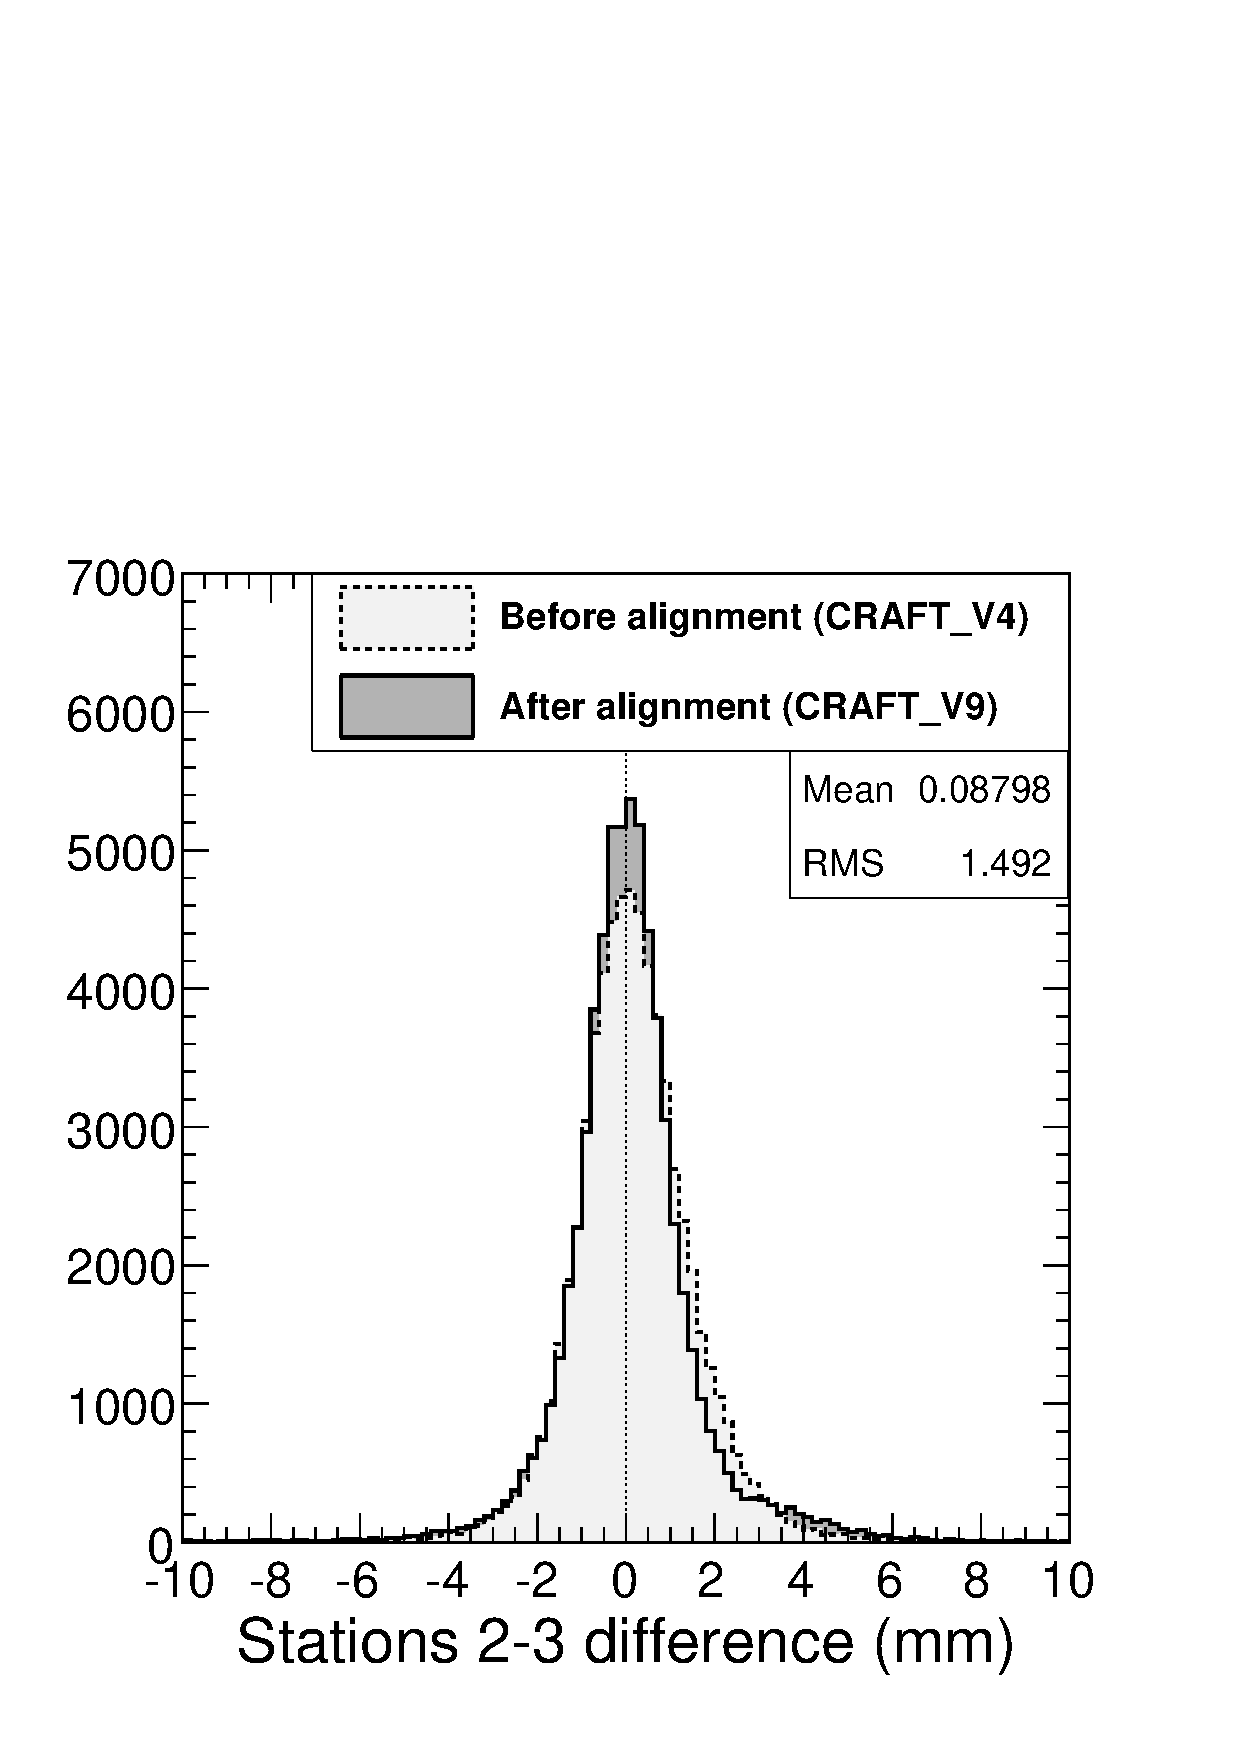
\includegraphics[width=0.25\linewidth]{residdiff23.pdf} \hfill 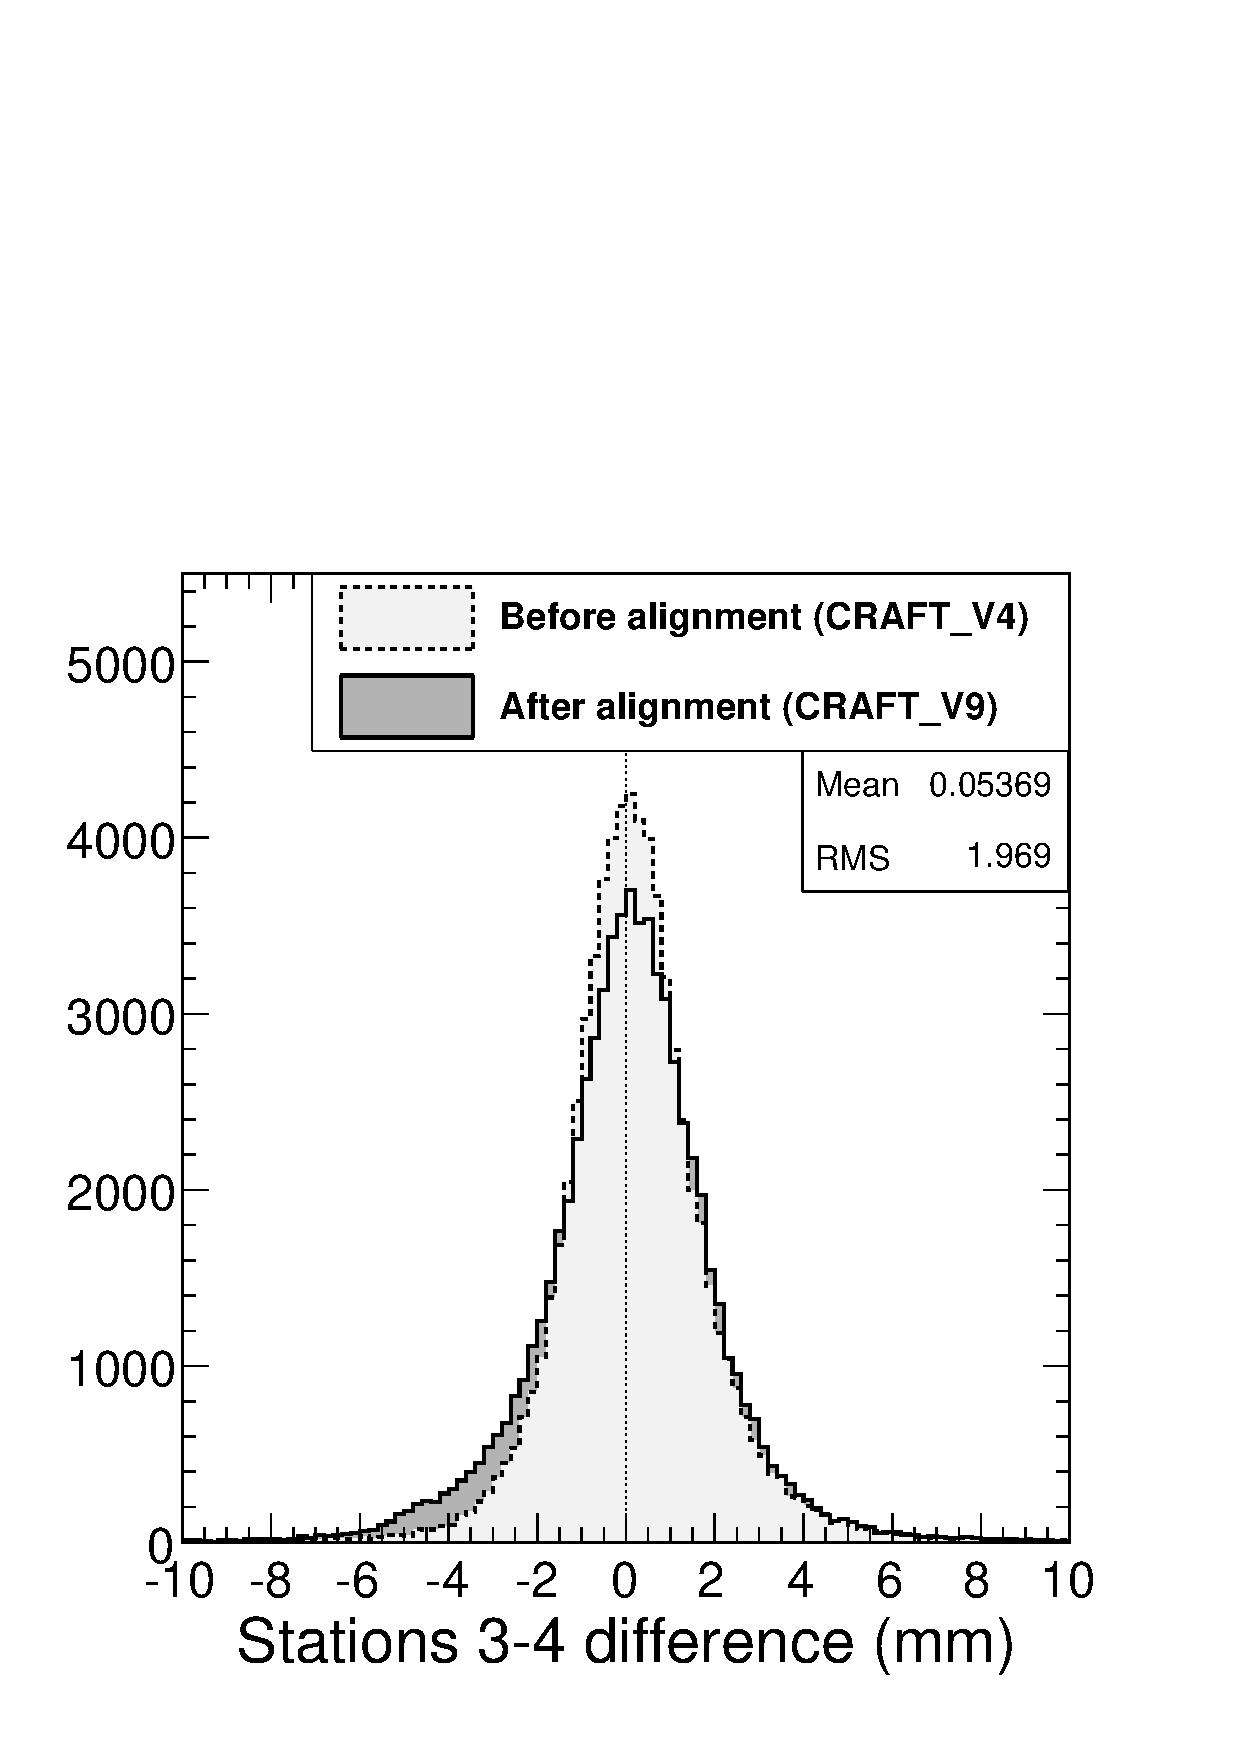
\includegraphics[width=0.25\linewidth]{residdiff34.pdf} \hfill \begin{minipage}{1 cm} \vspace{-1.3 cm} \tiny Note smaller scale \end{minipage} \mbox{ }

\vspace{0.3 cm}
\end{frame}

\begin{frame}
\frametitle{Cosmics track-splitting study}

\vspace{-0.05 cm}
\begin{columns}
\column{0.5\linewidth}
\begin{itemize}
\item Top and bottom half of a cosmic muon should have the same track parameters
\item GlobalMuon resolution worse than tracker-only for three reasons:
\begin{enumerate}
\item global misalignment
\item magnetic field errors
\item tracker given too little weight in global track fit
\end{enumerate}
\item Alignment improves matching of \mbox{$p_T > 100$~GeV cosmics\hspace{-1 cm}}
\begin{itemize}
\item insensitive to \textcolor{darkblue}{(2)}
\item plotted before \textcolor{darkblue}{(3)} \mbox{corrected\hspace{-1 cm}}
\end{itemize}
\item This is another cross-check because top-bottom agreement not used in \mbox{alignment procedure\hspace{-1 cm}}
\end{itemize}
\vspace{0.5 cm}

\column{0.6\linewidth}
\mbox{ } \hfill \textcolor{darkblue}{\scriptsize N.~Tran, A.~Bonato} \hfill \hfill \mbox{ }

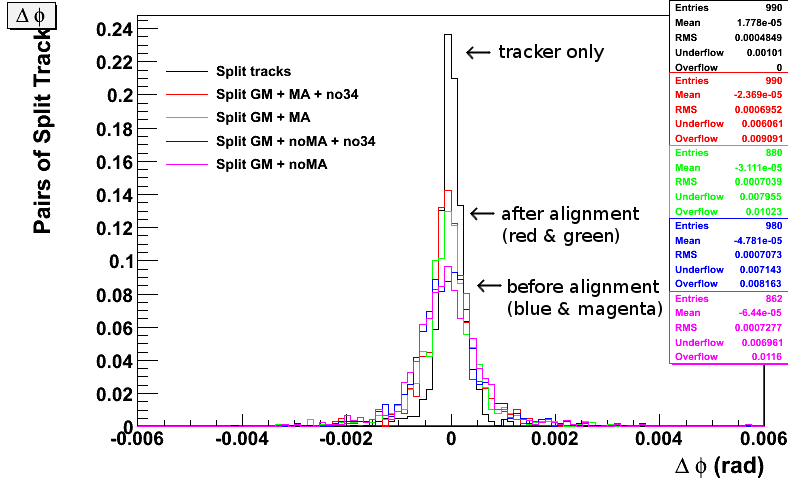
\includegraphics[width=\linewidth]{plots_dphi.png}

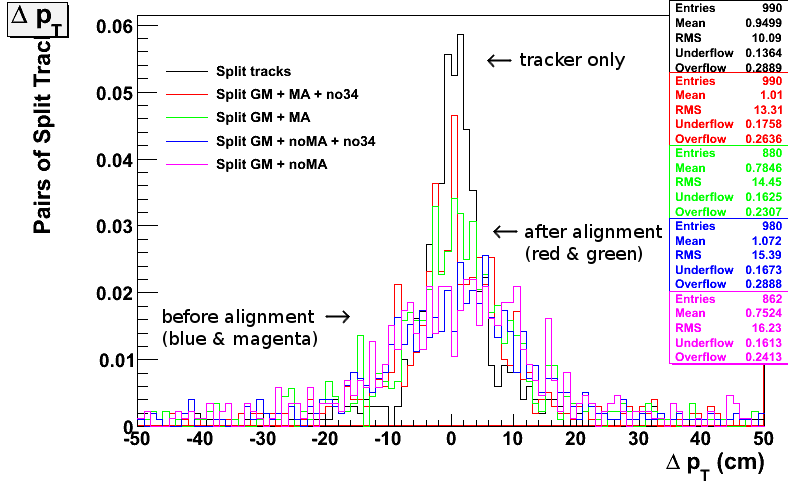
\includegraphics[width=\linewidth]{plots_dpt.png}
\end{columns}
\end{frame}

\begin{frame}
\frametitle{CSC alignment simulations}
\begin{itemize}
\item 50~pb$^{-1}$ of InclusiveMuPt10 (5$\times$ CSA08)
\item Statistical only, early tests, but results scale as $\sqrt{N}$ from CSA08
\item We now have reliable uncertainty estimates \mbox{(see normalized distributions)\hspace{-1 cm}}

and control for imperfect data: wrong $\vec{B}(\vec{x})$ and \mbox{non-Gaussian tails\hspace{-1 cm}}

\end{itemize}

\begin{columns}
\column{0.85\linewidth}
\begin{tabular}{p{0.3\linewidth} p{0.3\linewidth} p{0.3\linewidth}}
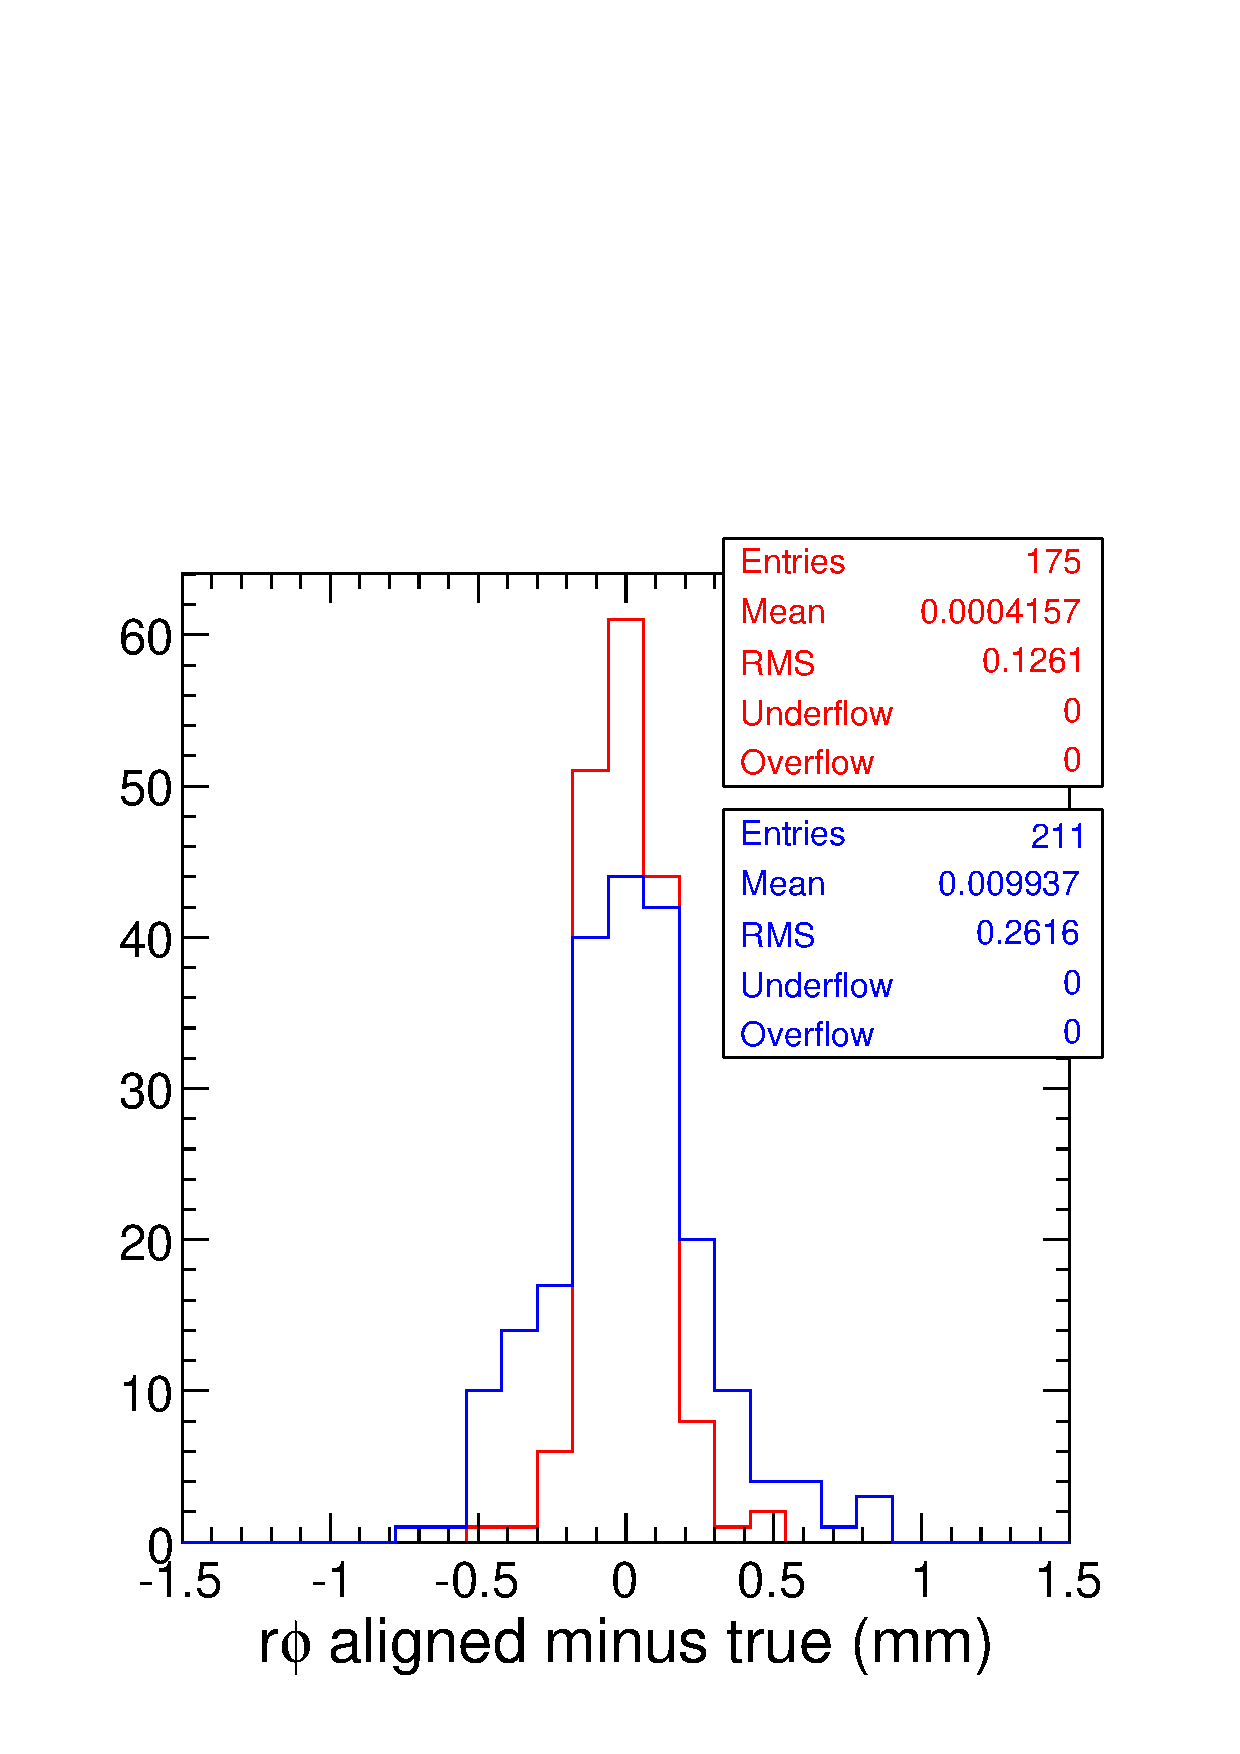
\includegraphics[width=\linewidth]{goodmodel_x.pdf} & 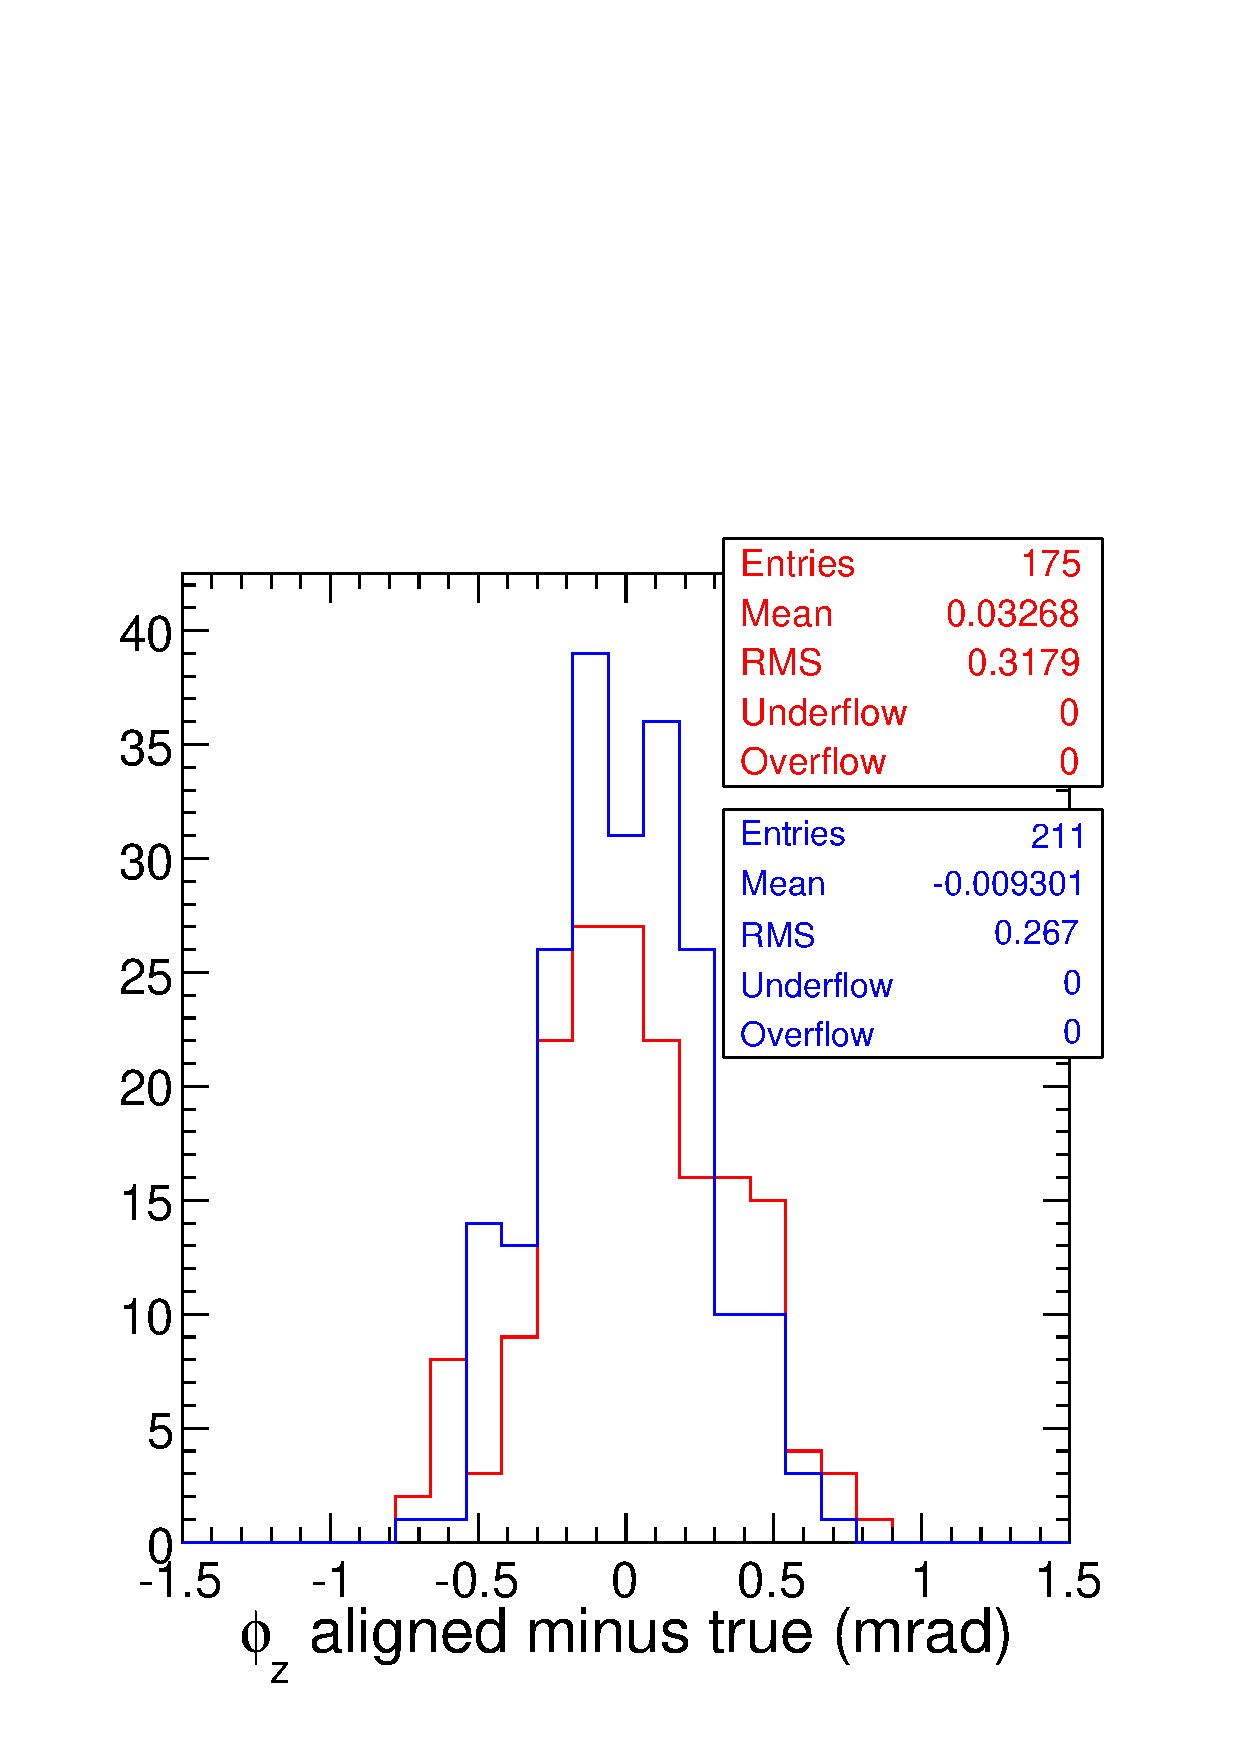
\includegraphics[width=\linewidth]{goodmodel_phiz.pdf} & 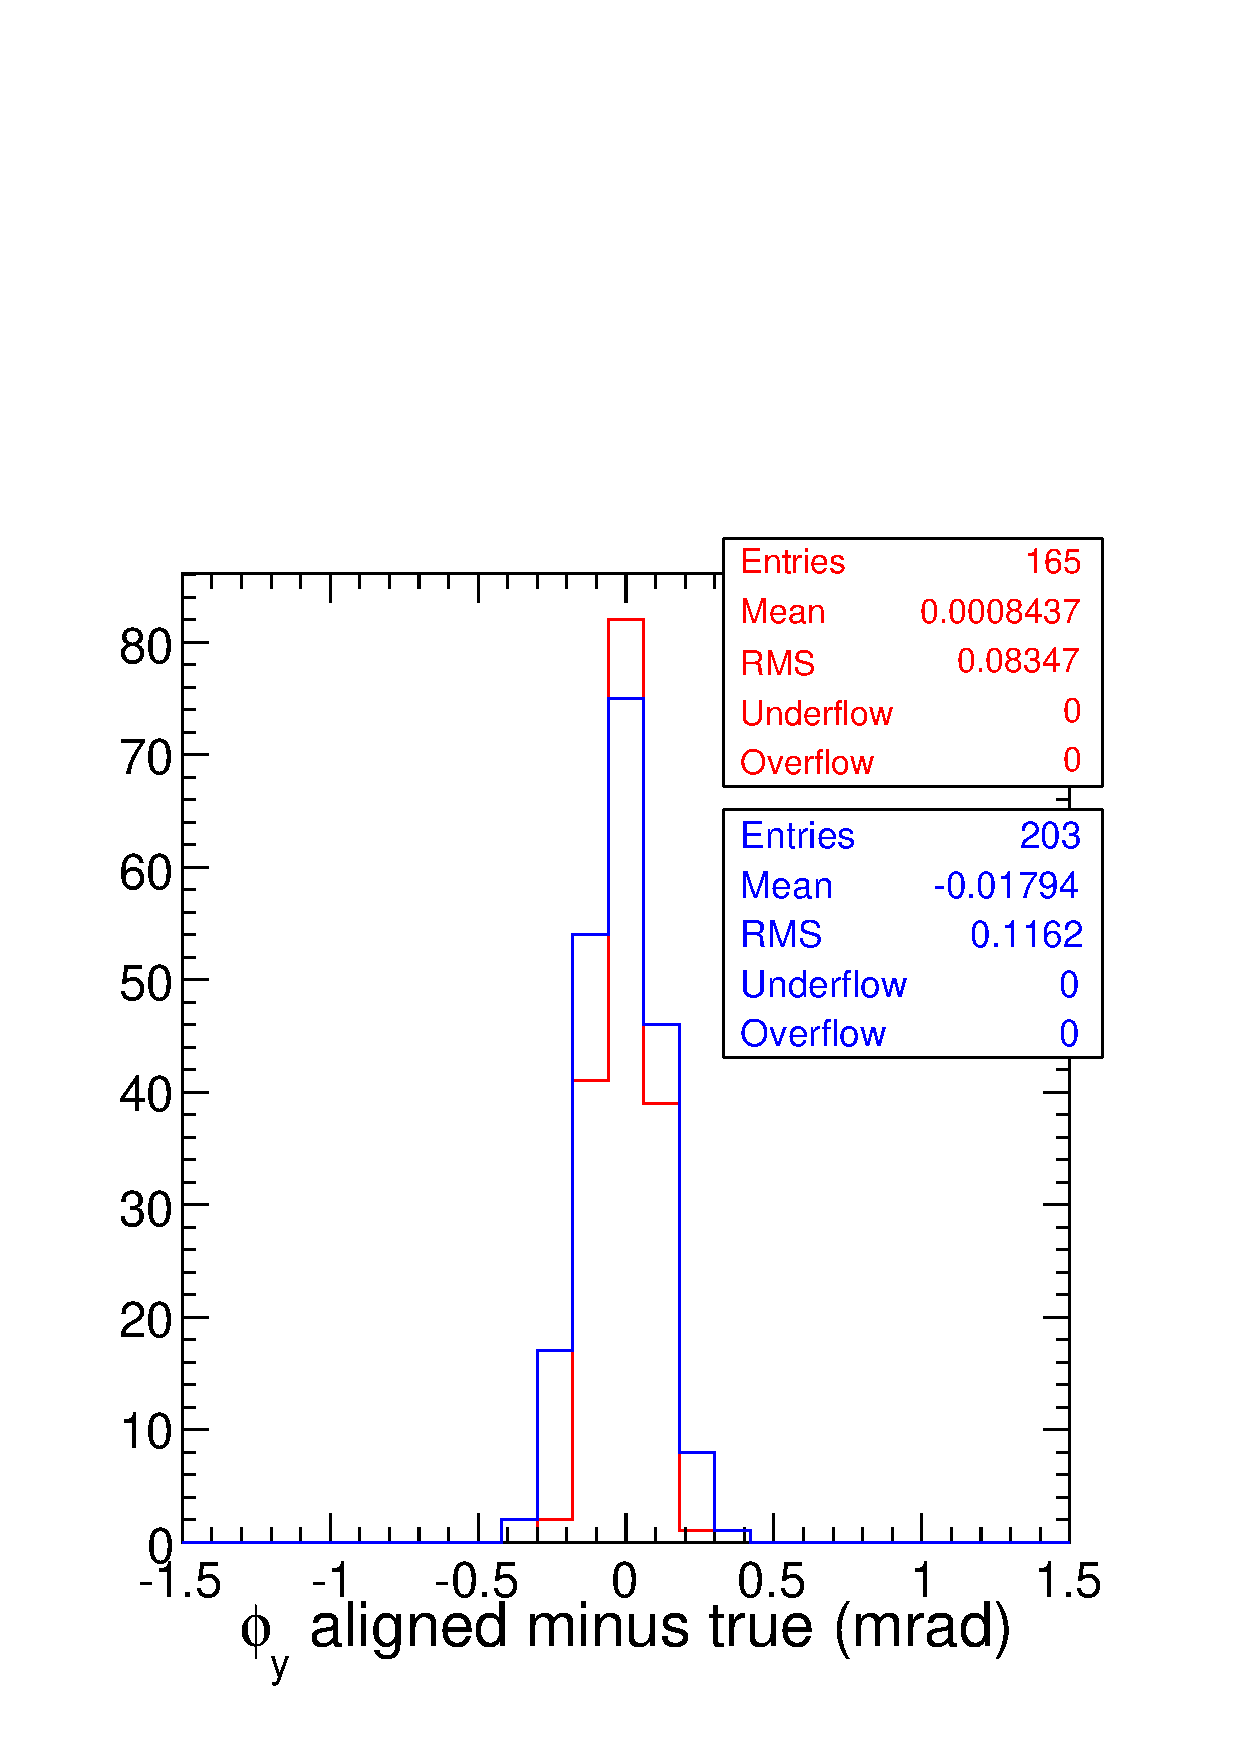
\includegraphics[width=\linewidth]{goodmodel_phiy.pdf} \\
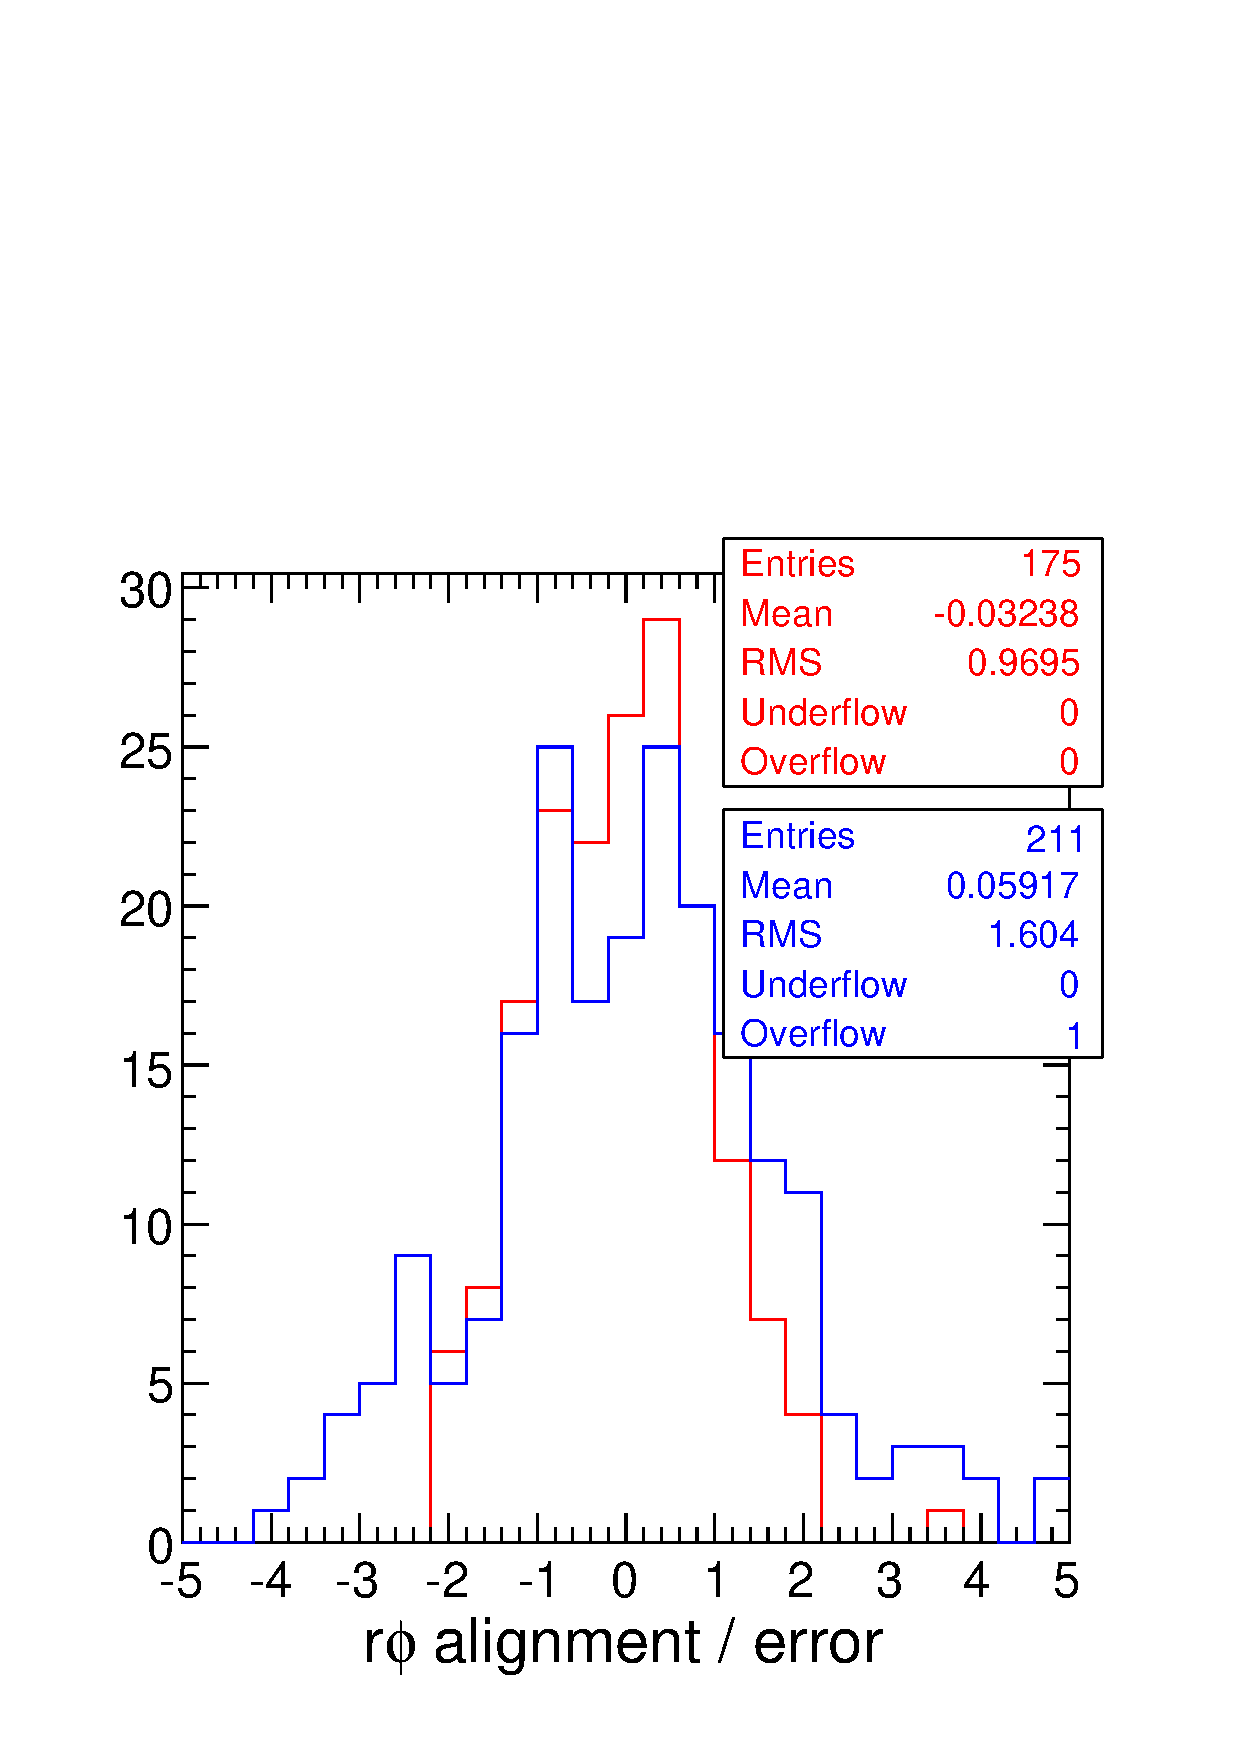
\includegraphics[width=\linewidth]{goodmodel_xnorm.pdf} & 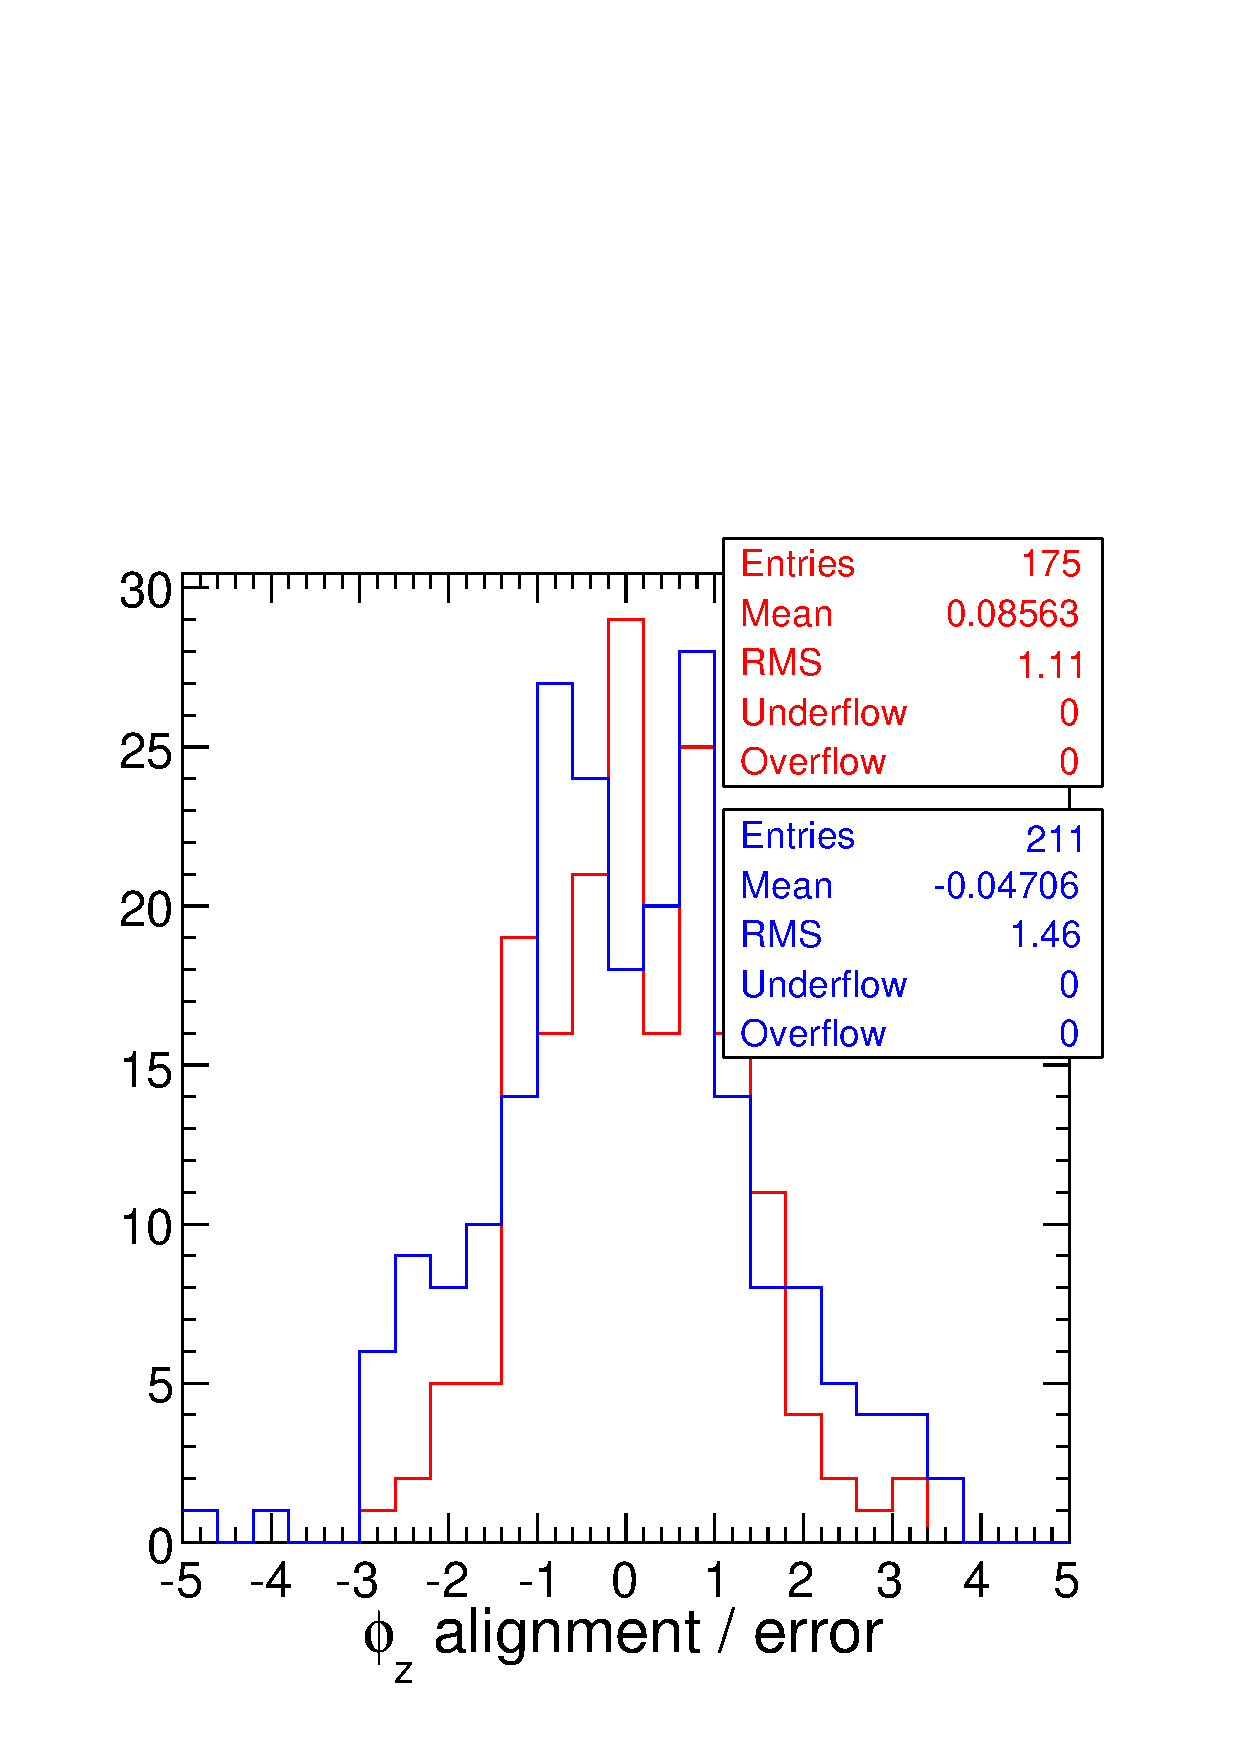
\includegraphics[width=\linewidth]{goodmodel_phiznorm.pdf} & 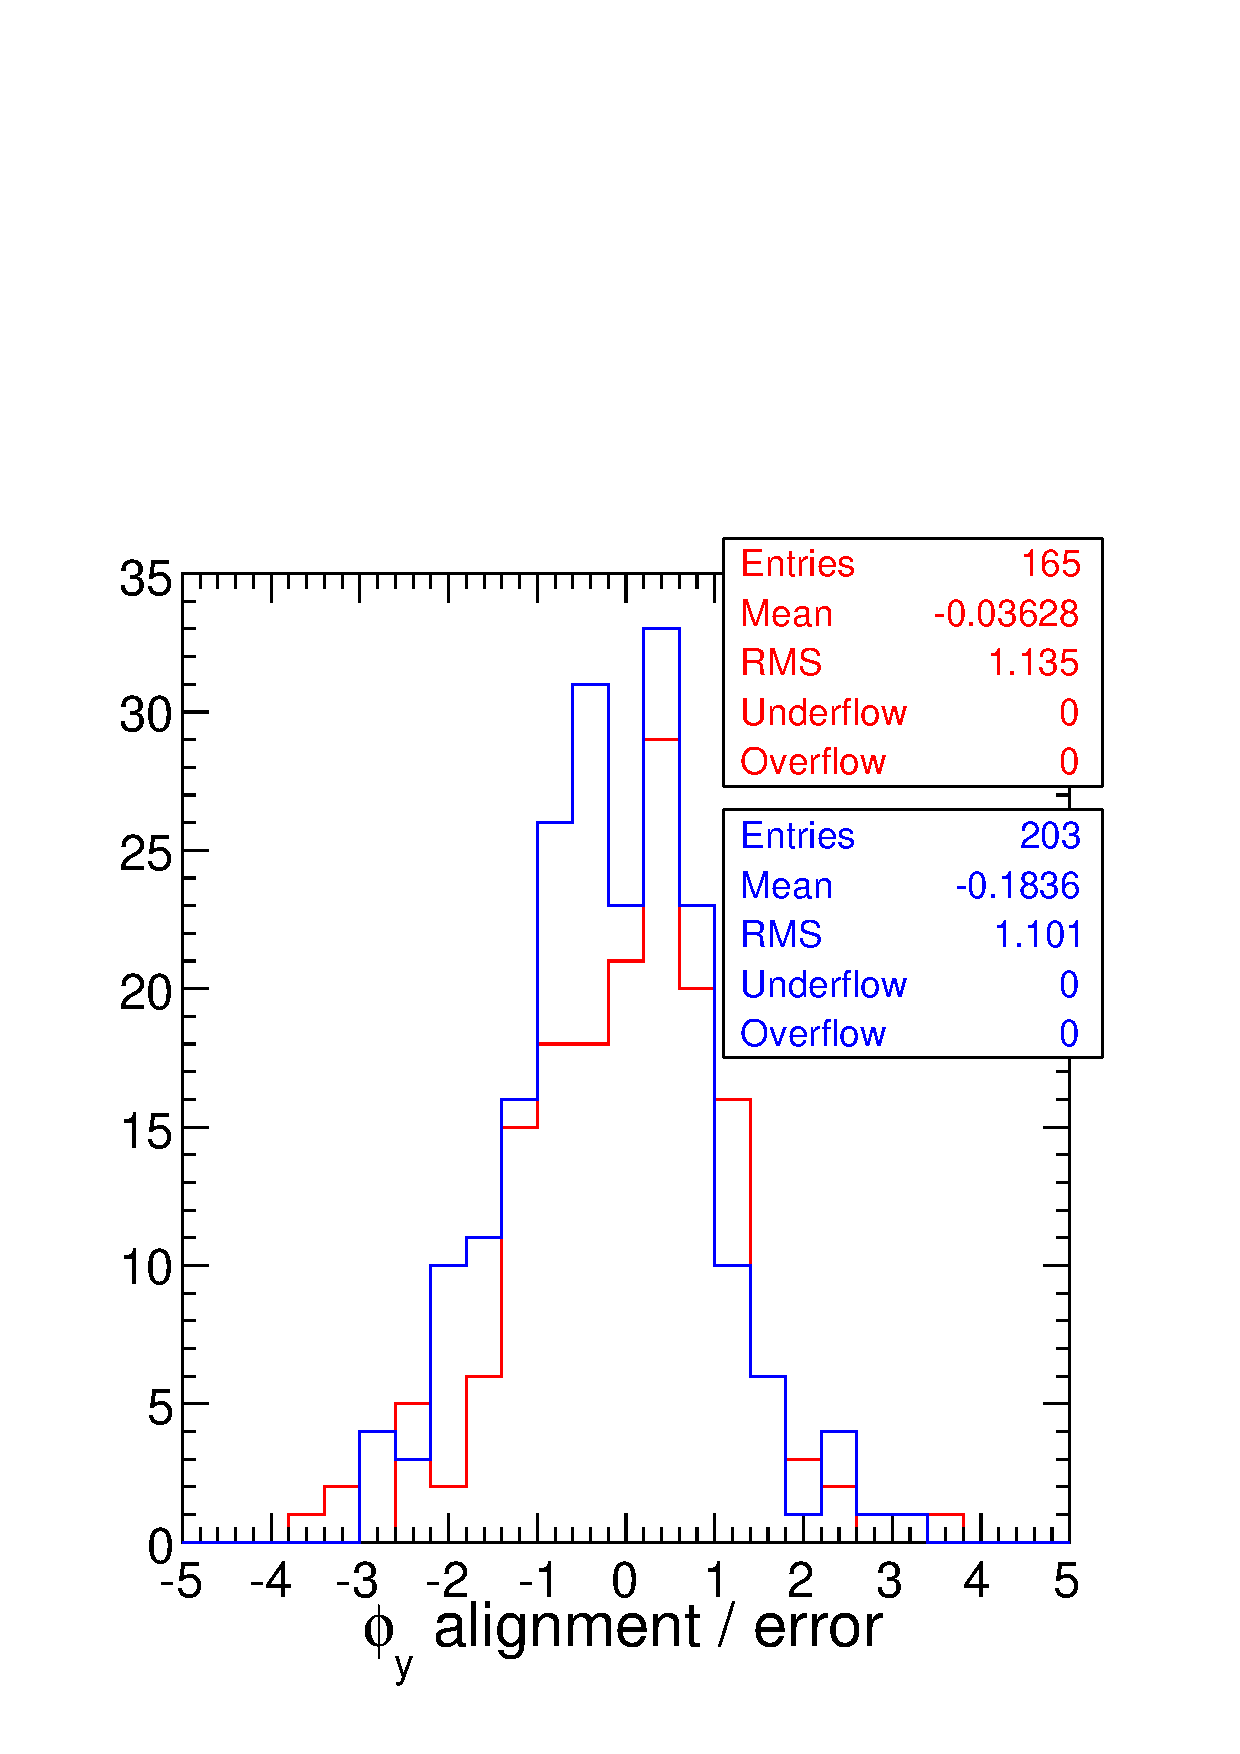
\includegraphics[width=\linewidth]{goodmodel_phiynorm.pdf}
\end{tabular}

\column{0.12\linewidth}
\tiny
PRELIMINARY!

\vspace{0.05 cm}
and statistical only

\vspace{0.25 cm}
\textcolor{red}{red is ring 1}
\textcolor{red}{\small 130~$\mu$m}

\vspace{0.25 cm}
\textcolor{blue}{blue is ring 2}
\textcolor{blue}{\small 260~$\mu$m}

\vspace{0.5 cm}
$z$ translation resolution under study

\vspace{1.5 cm}
\end{columns}
\end{frame}

\begin{frame}
\frametitle{Synergy with $\vec{B}(\vec{x})$ studies}

\begin{columns}
\column{0.35\linewidth}
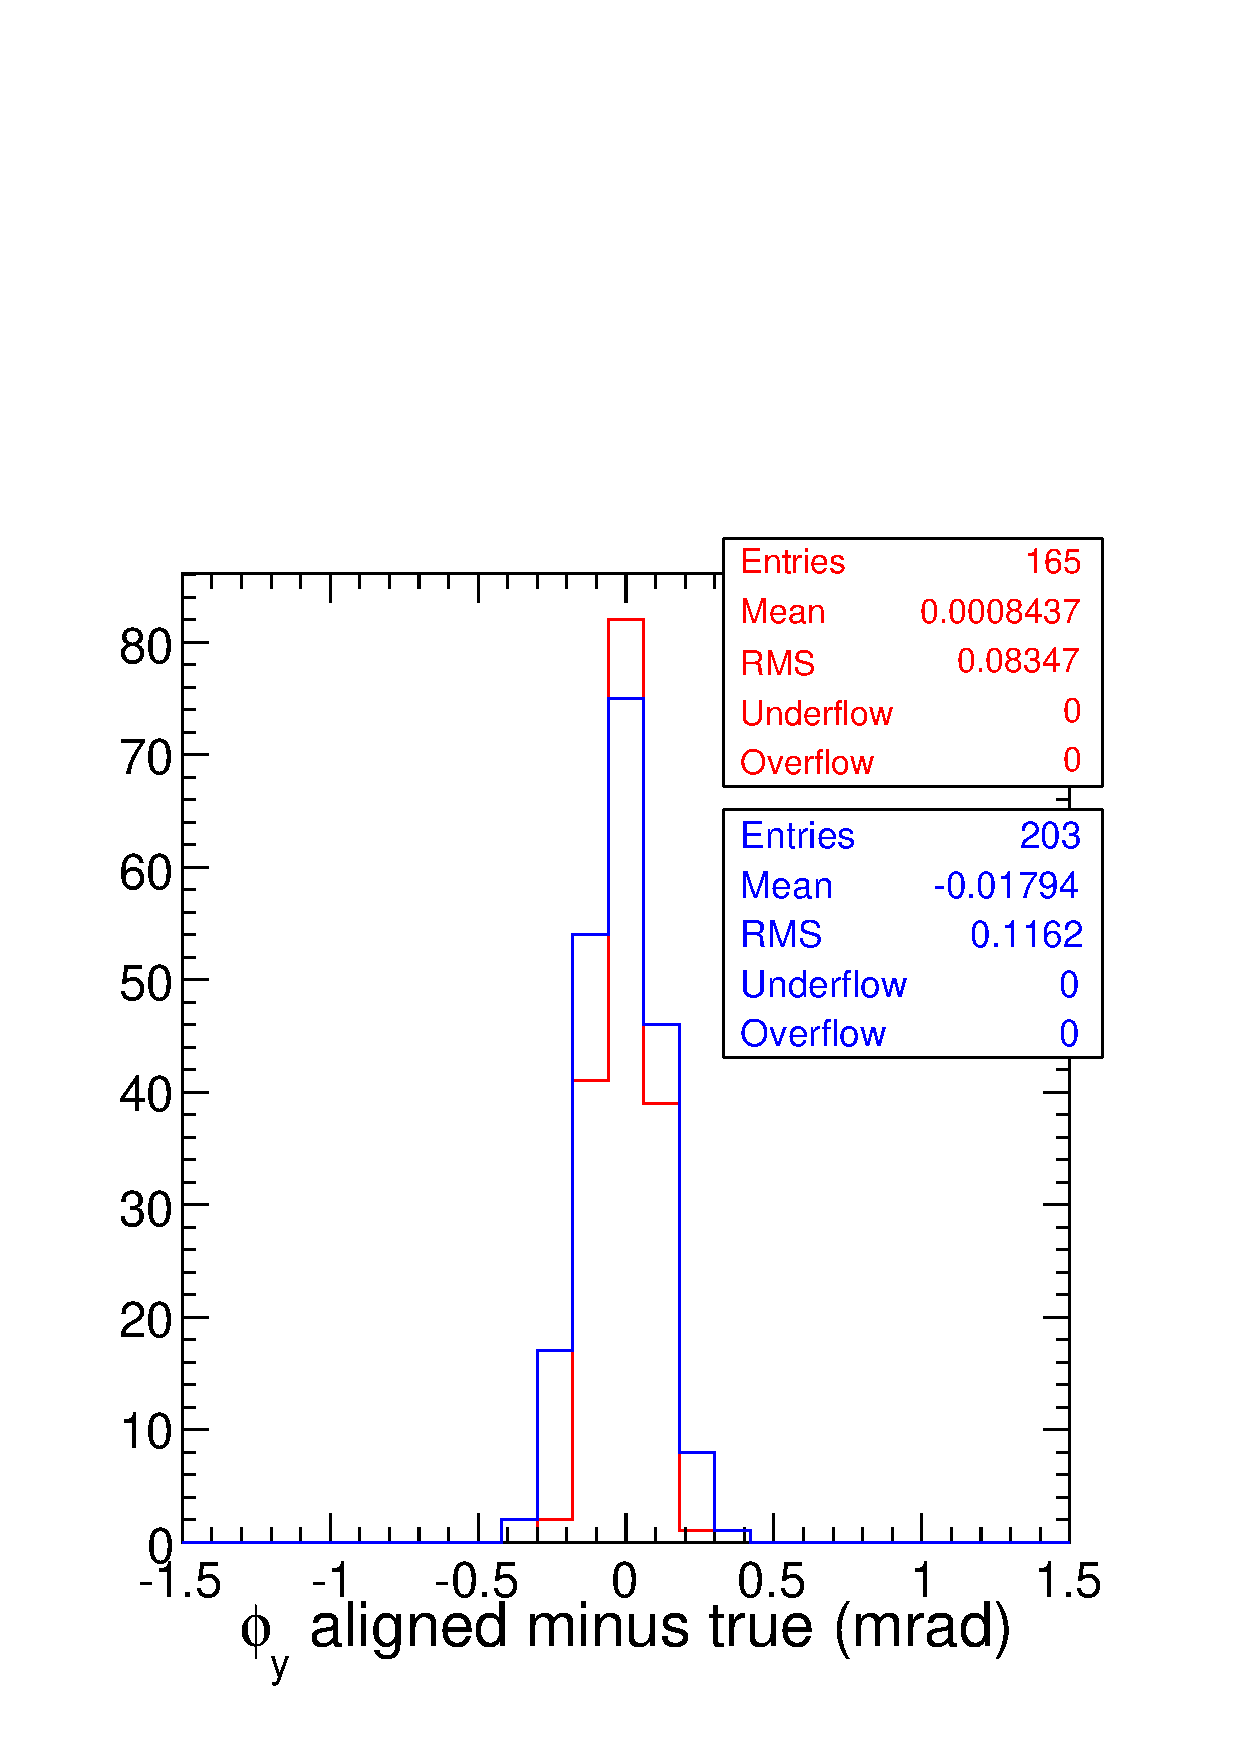
\includegraphics[width=\linewidth]{goodmodel_phiy.pdf}

\hfill 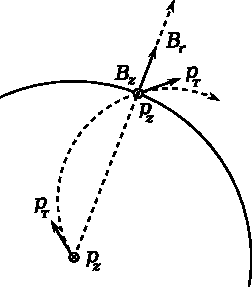
\includegraphics[width=0.8\linewidth]{bfield_components.pdf}
\column{0.7\linewidth}
\begin{itemize}
\item Best-measured parameter, $\phi_y$, is useful for measuring $\vec{B}(\vec{x})$ in the endcap

\vspace{-0.75 cm}
{\scriptsize
\begin{multline*}
\Delta \phi_y \, \approx \, \, \left(\phi_y\right)_{\mbox{\tiny misalignment}} + \\
\dfrac{R}{\mbox{\tiny 300 cm T/GeV}} \left[\left(\dfrac{q}{p_T}\right) \Delta B_z + \left(\dfrac{q}{p_z}\right) \Delta B_r \right] + \\
\mbox{\scriptsize ($dE/dx$ error)} \, \dfrac{q}{p^2}
\end{multline*}}

\vspace{-0.75 cm}
\item We'll need it: endcap $\vec{B}(\vec{x})$ is complicated\ldots
\end{itemize}

\hfill 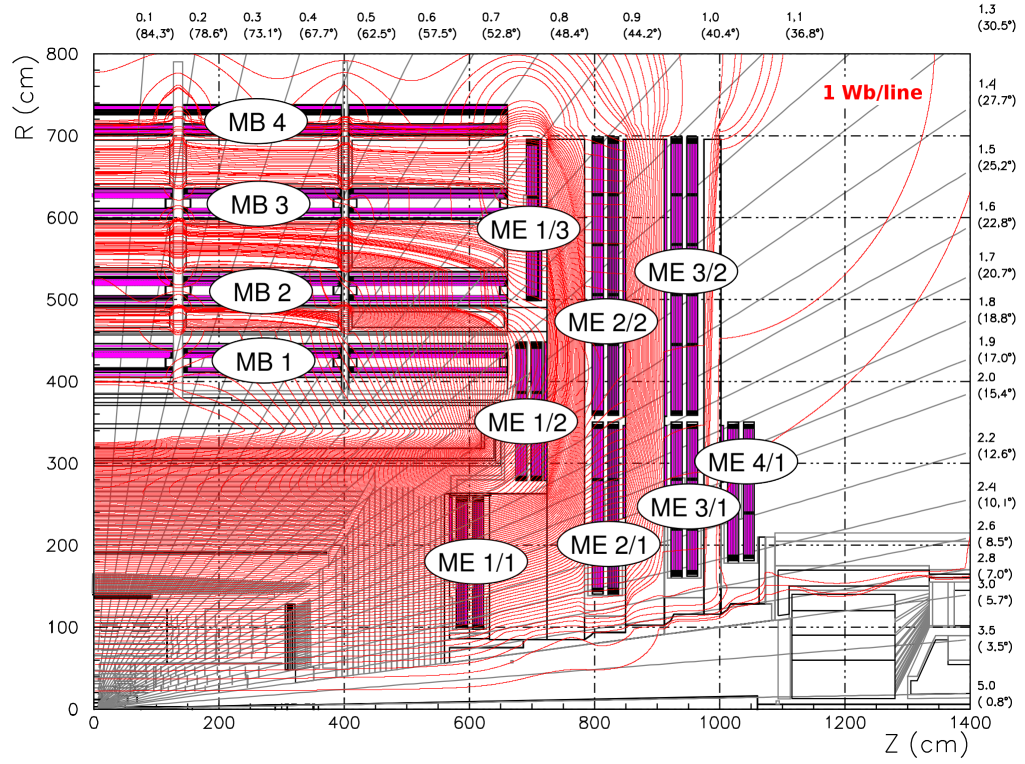
\includegraphics[width=0.8\linewidth]{muon_system_with_lines.png}

\end{columns}
\end{frame}

\begin{frame}
\frametitle{How do projects fit together?}

\begin{itemize}
\item The following are in progress or will be soon \hfill \textcolor{darkblue}{Goal: end of June}
\begin{itemize}
\item whole muon system alignment for \mbox{CRAFT-2008 analyses\hspace{-1 cm}}
\item automated software/plots ready for CRAFT-2009 \mbox{beam-prep run\hspace{-1 cm}}
\item well-documented CMS Note to ease new-member transition
\item 200~pb$^{-1}$ misalignment scenario for first physics analyses
\end{itemize}
\end{itemize}

\mbox{\hspace{-0.75 cm}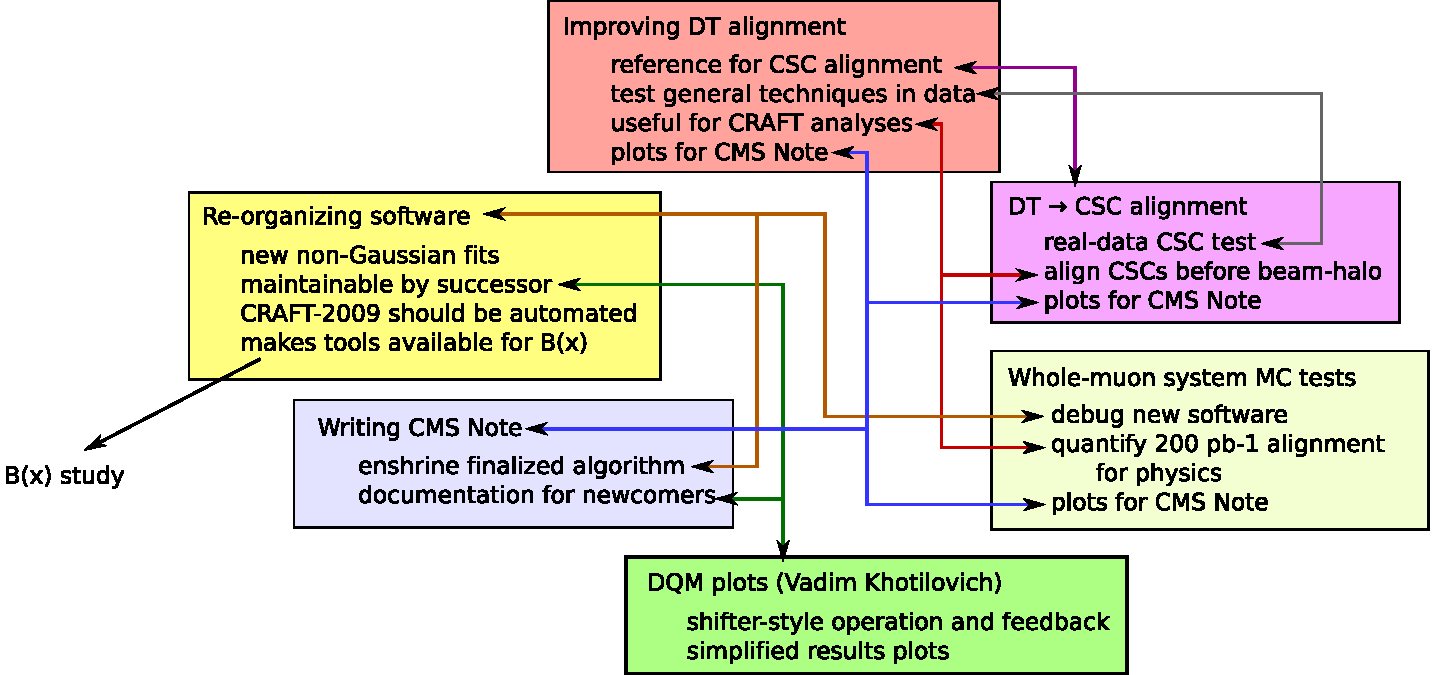
\includegraphics[width=1.1\linewidth]{connections.pdf}}

\end{frame}

\begin{frame}
\frametitle{Timeline for track-based}
\vfill
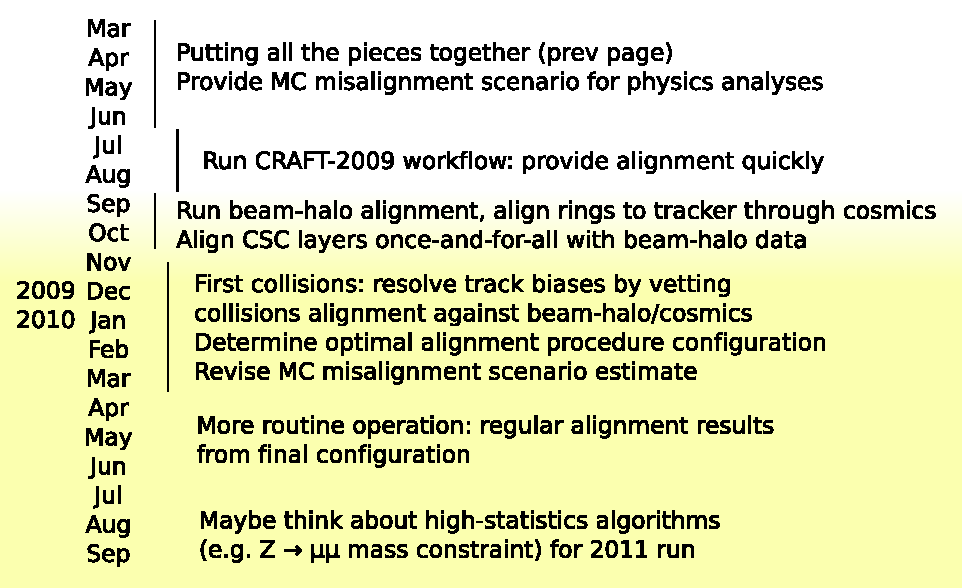
\includegraphics[width=\linewidth]{timeline.pdf}

\vfill
\end{frame}

\begin{frame}
\frametitle{Merging alignment information}
\begin{itemize}
\item Every alignment procedure has parameters it measures well and parameters it doesn't
\begin{itemize}
\item CSC Overlaps: $x$, $\phi_y$, $\phi_z$ relative to ring
\item SLM: $x$, $z$, $\phi_x$ for monitored chambers relative to disk
\item Tracker-to-muon: $x$, $z$, $\phi_y$, $\phi_z$ globally
\end{itemize}

\item They can be sequentially chained if each does the following
\begin{enumerate}
\item read a geometry from a CSCAlignmentRcd
\item modify what it measures well by relative transformations
\item write the updated geometry to a CSCAlignmentRcd
\end{enumerate}
\end{itemize}

\textcolor{darkblue}{Simplified example:} suppose it is determined that SLM $z$ information is more
accurate than track-based (through extensive cross-checks)

\begin{center}
\begin{columns}
\column{0.1\linewidth}

\column{0.5\linewidth}
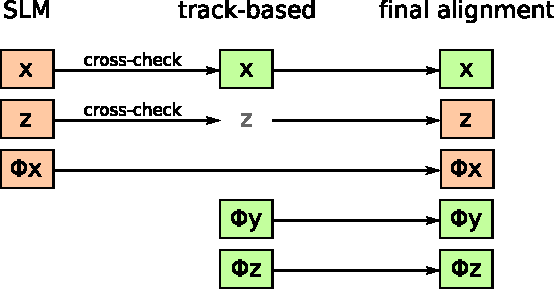
\includegraphics[width=\linewidth]{merging_information.pdf}

\column{0.4\linewidth}
Much easier to understand the systematics of the final alignment and estimate its uncertainty for \mbox{physics analyses\hspace{-1 cm}}

\vspace{0.25 cm}
Global fit would obscure that
\end{columns}
\end{center}
\end{frame}

\begin{frame}
\frametitle{Conclusions}

\begin{itemize}\setlength{\itemsep}{0.1 cm}
\item CRAFT taught what real data looks like with \mbox{high statistics\hspace{-1 cm}}
\begin{itemize}\setlength{\itemsep}{0.1 cm}
\item tested new techniques to disentangle $\vec{B}(\vec{x})$ effects
  from misalignment
\item got to know our residuals better
\item discovered a strange feature in $r\phi$ residual versus $\phi$ (page~\pageref{page:rphivsphi})
\item could only study DTs so far because there's a \mbox{tracker $\to$ DT $\to$ CSC dependency} with cosmic rays
\end{itemize}

\item Produced a partial barrel alignment (and corresponding MC
  misalignment scenario) for physics analyses, \mbox{passes cross-checks\hspace{-1 cm}}

\item Consolidating experiences into revised software, documentation,
  and an updated estimate for resolution at 200~pb$^{-1}$

\item CRAFT-2008 was about learning a new environment; CRAFT-2009 should be routine

\item We'll have more to think about with first collisions, but
  cross-checks/systematics-study era will give way to routine
  era
\end{itemize}

\label{numpages}
\end{frame}

\end{document}
